\documentclass[table]{beamer}
\mode<presentation>
\usetheme{Berlin}
\usecolortheme{beaver}
\usepackage{upquote} % Protect single quotes in code listings
\usepackage{listings}
\usepackage{multirow}
\usepackage{xcolor}

%%%
% LISTINGS SETTING
\lstset{ %
  backgroundcolor=\color{yellow},   % choose the background color; you must add \usepackage{color} or \usepackage{xcolor}
  basicstyle=\tiny\ttfamily,        % the size of the fonts that are used for the code
  breakatwhitespace=false,         % sets if automatic breaks should only happen at whitespace
  breaklines=true,                 % sets automatic line breaking
  captionpos=b,                    % sets the caption-position to bottom
  commentstyle=\color{red},    % comment style
  deletekeywords={...},            % if you want to delete keywords from the given language
  escapeinside={\%*}{*)},          % if you want to add LaTeX within your code
  extendedchars=true,              % lets you use non-ASCII characters; for 8-bits encodings only, does not work with UTF-8
  frame=single,                    % adds a frame around the code
  keepspaces=true,                 % keeps spaces in text, useful for keeping indentation of code (possibly needs columns=flexible)
  keywordstyle=\color{blue},       % keyword style
%  language=Octave,                 % the language of the code
  morekeywords={*,...},            % if you want to add more keywords to the set
  numbers=left,                    % where to put the line-numbers; possible values are (none, left, right)
  numbersep=5pt,                   % how far the line-numbers are from the code
  numberstyle=\tiny\color{gray}, % the style that is used for the line-numbers
  rulecolor=\color{black},         % if not set, the frame-color may be changed on line-breaks within not-black text (e.g. comments (green here))
  showspaces=false,                % show spaces everywhere adding particular underscores; it overrides 'showstringspaces'
  showstringspaces=false,          % underline spaces within strings only
  showtabs=false,                  % show tabs within strings adding particular underscores
  stepnumber=1,                    % the step between two line-numbers. If it's 1, each line will be numbered
  stringstyle=\color{violet},     % string literal style
  tabsize=4,                       % sets default tabsize to 2 spaces
  title=\lstname                   % show the filename of files included with \lstinputlisting; also try caption instead of title
}


%%%
% TITLE PREAMBLE
\title[Intro to Bioinformatics] % (optional, only for long titles)
{An Introduction to Bioinformatics Tools}
\subtitle{Part 3: Workshop}
\author[Pritchard, Cock] % (optional, for multiple authors)
{Leighton~Pritchard \and Peter~Cock}
\institute[The James Hutton Institute] % (optional)
{
  Information and Computational Sciences\\
  The James Hutton Institute
}
\date[May 2014] % (optional)
{Bioinformatics Training, 29$^{th}$, 30$^{th}$ May 2014}
\subject{Bioinformatics}

%%%
% TOC
% Show table of contents, with current section highlighted,
% at the start of each section
\AtBeginSection[]
{
  \begin{frame}
    \frametitle{Table of Contents}
    \tableofcontents[currentsection,hideallsubsections]
  \end{frame}
}


%%%
% START DOCUMENT
\begin{document}

  \frame[plain]{\titlepage}
 
    \begin{frame}
     \frametitle{Learning Outcomes}
     \begin{itemize}
       \item Workshop example: bacterial genome annotation
       \begin{itemize}
         \item The role of biological insight in a bioinformatics workflow
         \item Getting data from remote sources
         \item Visual interaction with sequence data
         \item Using alternative tools
         \item Comparison of tools and outputs
         \item Online tools for automated function prediction
       \end{itemize}
     \end{itemize}
    \end{frame} 
  
%%%
% SECTION: Workshop Outline
\section{Outline}

    % What you will be doing
    \begin{frame}
     \frametitle{What You Will Be Doing}
     Illustrative example of concepts
     \begin{itemize}
       \item Functional annotation of a draft bacterial genome
       \begin{itemize}
         \item Gene prediction/ORF detection
         \item Genome comparisons
         \item Gene functional annotation
         \item Gene comparisons
       \end{itemize}
     \end{itemize}
    \end{frame}

    \begin{frame}
     \frametitle{Gene (coding sequence) Prediction}
     \begin{itemize}
       \item ORF detection
       \item Glimmer
       \item Prodigal
       \item Benchmarking gene prediction
       \item Artemis
     \end{itemize}
    \end{frame}
    
    \begin{frame}
     \frametitle{Genome comparisons}
     \begin{itemize}
       \item BLAST
       \item MUMmer
       \item ACT
       \item (Mauve)
       \item Differences between genome aligners
     \end{itemize}
    \end{frame}

    \begin{frame}
     \frametitle{Functional Prediction}
     \begin{itemize}
       \item InterPro
       \item RAST
       \item (KAAS)
       \item PFam
       \item Artemis
       \item Functional classification
     \end{itemize}
    \end{frame}
    
    \begin{frame}
     \frametitle{Gene Comparisons}
     \begin{itemize}
       \item BLAST
       \item (HMMer)
       \item CLUSTAL
       \item T-COFFEE
       \item JalView
       \item Differences between gene aligners
     \end{itemize}
    \end{frame}


  % Getting started
  \section{Load Sequence Data}
  \begin{frame}
    \frametitle{Locate your data}
    \begin{itemize}
      \item You are in group A, B, C or D - this decides your chromosome sequence: \\
      \texttt{chrA.fasta}, \texttt{chrB.fasta}, \texttt{chrC.fasta}, \texttt{chrD.fasta}
      \item Each sequence represents a single stitched, ordered draft bacterial genome comprising a number of contigs.
      \item You will use your sequence as the basis of the exercises in the workshop.
    \end{itemize}
  \end{frame}
  
  \begin{frame}
    \frametitle{Locate your data}
    \begin{itemize}
      \item You are in group A, B, C or D - this decides your dataset: \\
      \texttt{chrA.fasta}, \texttt{chrB.fasta}, \texttt{chrC.fasta}, \texttt{chrD.fasta}
      \item You also have a GFF file describing the location of assembled contigs \\
      \texttt{chrA\_contigs.gff}, \texttt{chrB\_contigs.gff}, \texttt{chrC\_contigs.gff}, \texttt{chrD\_contigs.gff}
      \item Your data is in \texttt{data/workshop/chromosomes}
    \end{itemize}
  \end{frame}
  
% [fragile] frames must end with \end{frame} directly following a newline, or they break!
\begin{frame}[fragile]
\frametitle{Inspect the data}
\begin{lstlisting}[language=]
$ head -n 3 chrA.fasta 
>chrA
ttttcttgattgaccttgttcgagtggagtccgccgtgtcactttcgctttggcagcagt
gtcttgcccgtttgcaggatgagttacctgccacagaattcagtatgtggatacgcccgt
$ head -n 3 chrA_contigs.gff 
##gff-version 3
chrA	stitching	contig	1	154993	.	.	.	ID=contig00005_b;Name=contig00005_b
chrA	stitching	contig	155036	241491	.	.	.	ID=contig00018;Name=contig00018
\end{lstlisting}
\end{frame}

% [fragile] frames must end with \end{frame} directly following a newline, or they break!
\begin{frame}[fragile]
\frametitle{Download a Comparator Sequence}
\texttt{wget} is a powerful command-line tool for downloading data
\begin{lstlisting}[language=]
$ wget ftp://ftp.ncbi.nih.gov/genomes/Bacteria/Pectobacterium_atrosepticum_SCRI1043_uid57957/NC_004547.fna
--2014-05-27 13:35:05--  ftp://ftp.ncbi.nih.gov/genomes/Bacteria/Pectobacterium_atrosepticum_SCRI1043_uid57957/NC_004547.fna
           => 'NC_004547.fna'
Resolving ftp.ncbi.nih.gov... 130.14.250.7, 2607:f220:41e:250::12
Connecting to ftp.ncbi.nih.gov|130.14.250.7|:21... connected.
Logging in as anonymous ... Logged in!
==> SYST ... done.    ==> PWD ... done.
==> TYPE I ... done.  ==> CWD (1) /genomes/Bacteria/Pectobacterium_atrosepticum_SCRI1043_uid57957 ... done.
==> SIZE NC_004547.fna ... 5136458
==> PASV ... done.    ==> RETR NC_004547.fna ... done.
Length: 5136458 (4.9M) (unauthoritative)

100%[=====================>] 5,136,458    562KB/s   in 7.7s 
$ ls NC*
NC_004547.fna
\end{lstlisting}
\end{frame}


  % Artemis
  \subsection{Artemis}
% [fragile] frames must end with \end{frame} directly following a newline, or they break!
  \begin{frame}[fragile]
    \frametitle{Inspect the data}
    Starting \texttt{Artemis}
\begin{lstlisting}[language=bash]
$ art &
\end{lstlisting}
    \begin{center}
      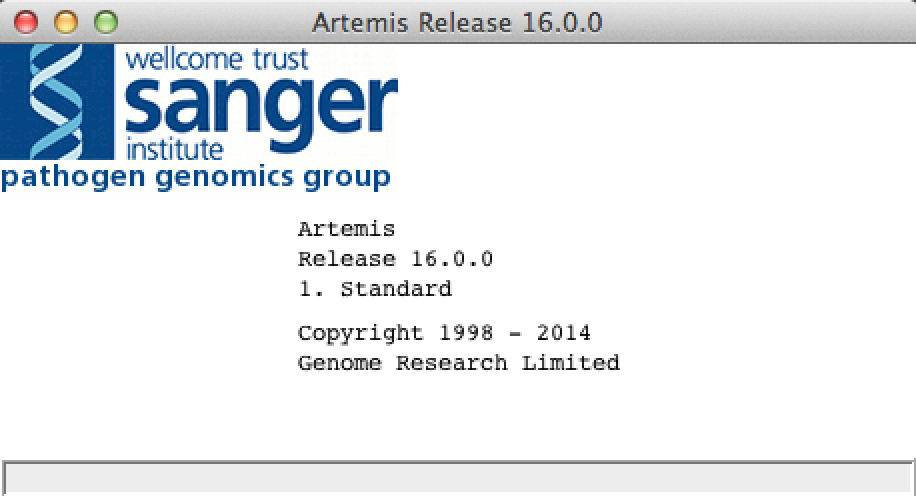
\includegraphics[width=0.6\textwidth]{images/artemis_splash} 
    \end{center}
\end{frame}
    
  \begin{frame}
    \frametitle{Load the chromosome sequence}
    Select the sequence for your group
    \begin{center}
      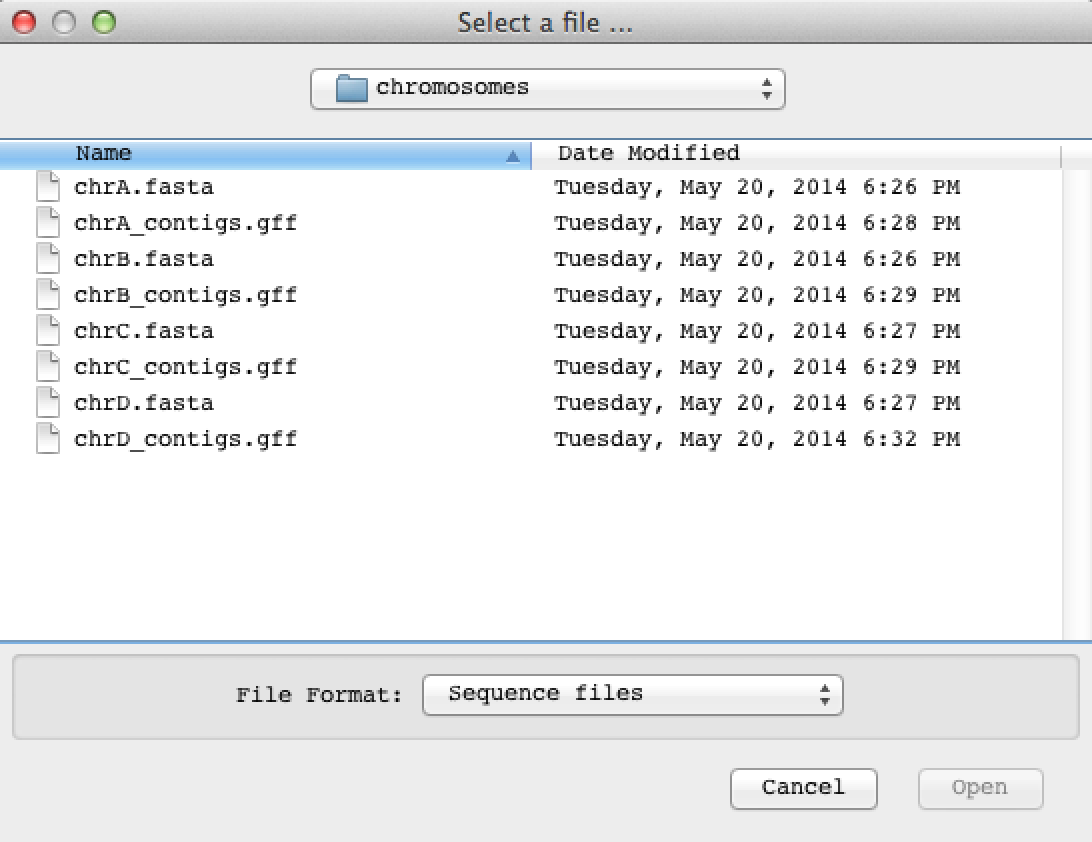
\includegraphics[width=0.7\textwidth]{images/artemis_files} 
    \end{center}
\end{frame}
    
  \begin{frame}
    \frametitle{Load the chromosome sequence}
    \begin{center}
      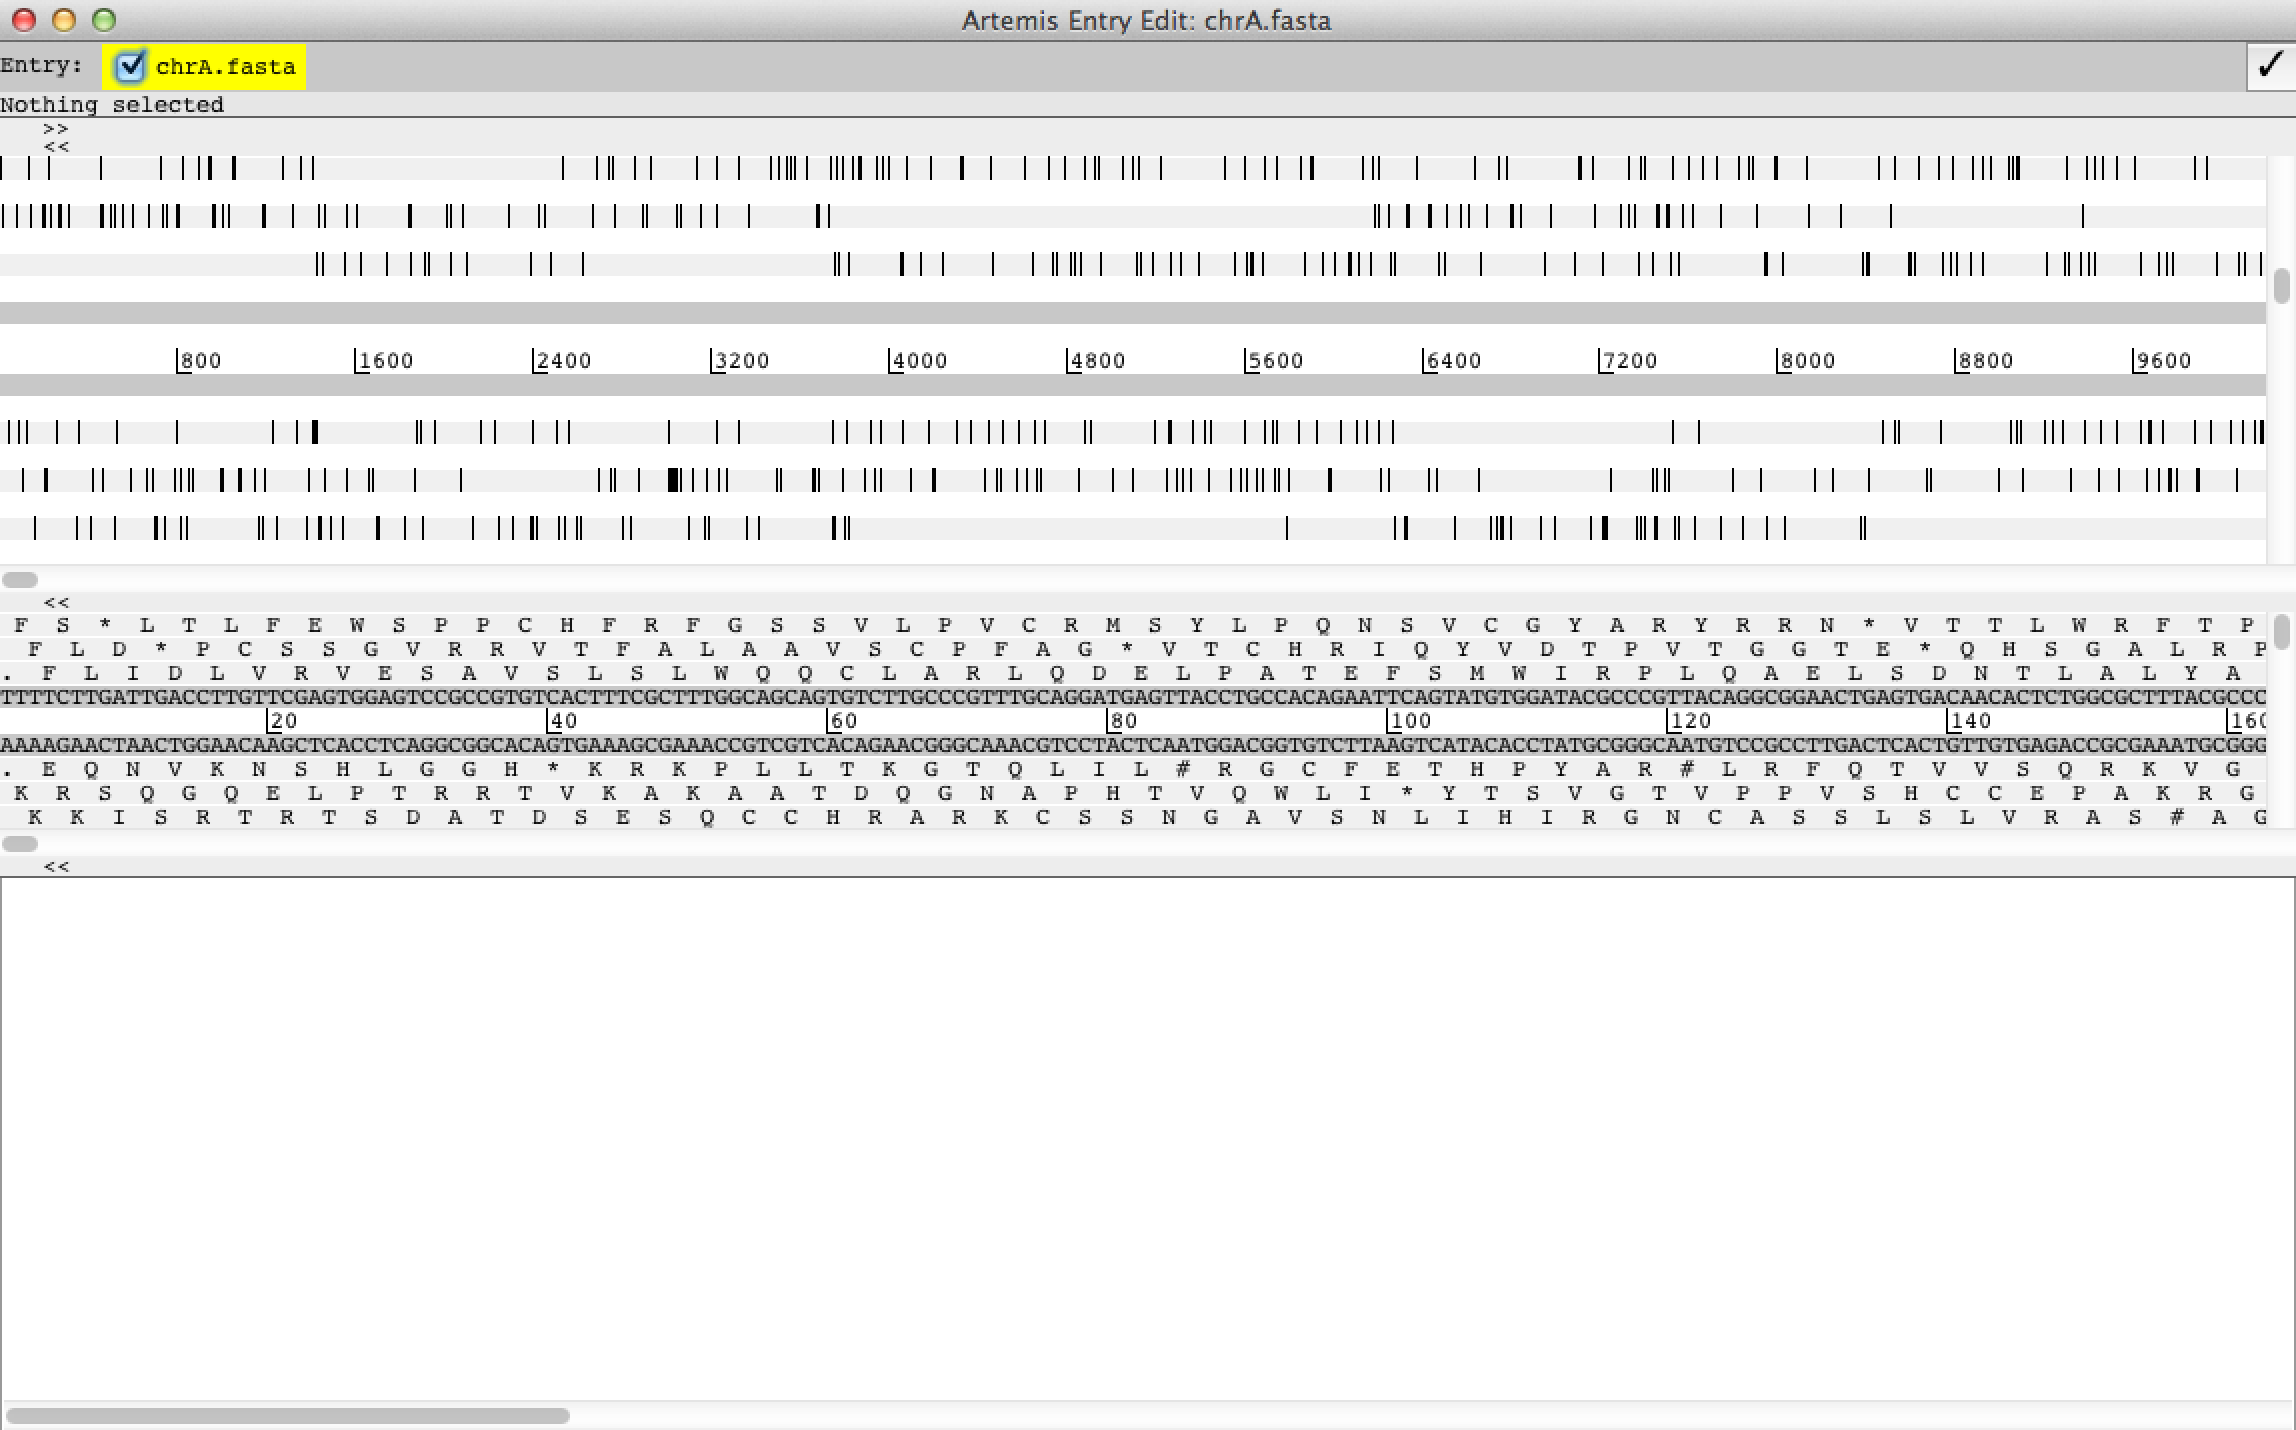
\includegraphics[width=0.8\textwidth]{images/artemis_loaded_seq} 
    \end{center}
\end{frame}

  \begin{frame}
    \frametitle{Load the contig GFF}
    \begin{center}
      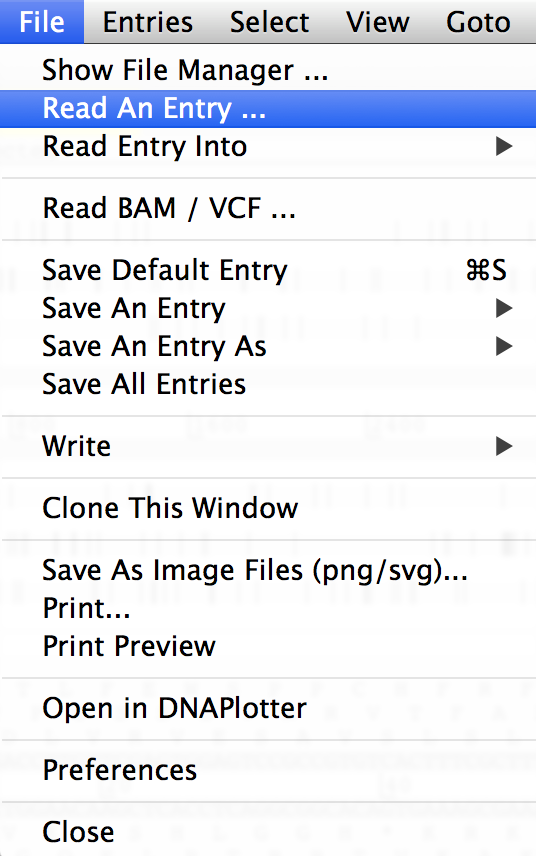
\includegraphics[width=0.3\textwidth]{images/artemis_read_entry} 
    \end{center}
\end{frame}

  \begin{frame}
    \frametitle{Load the contig GFF}
    Select the file for your group
    \begin{center}
      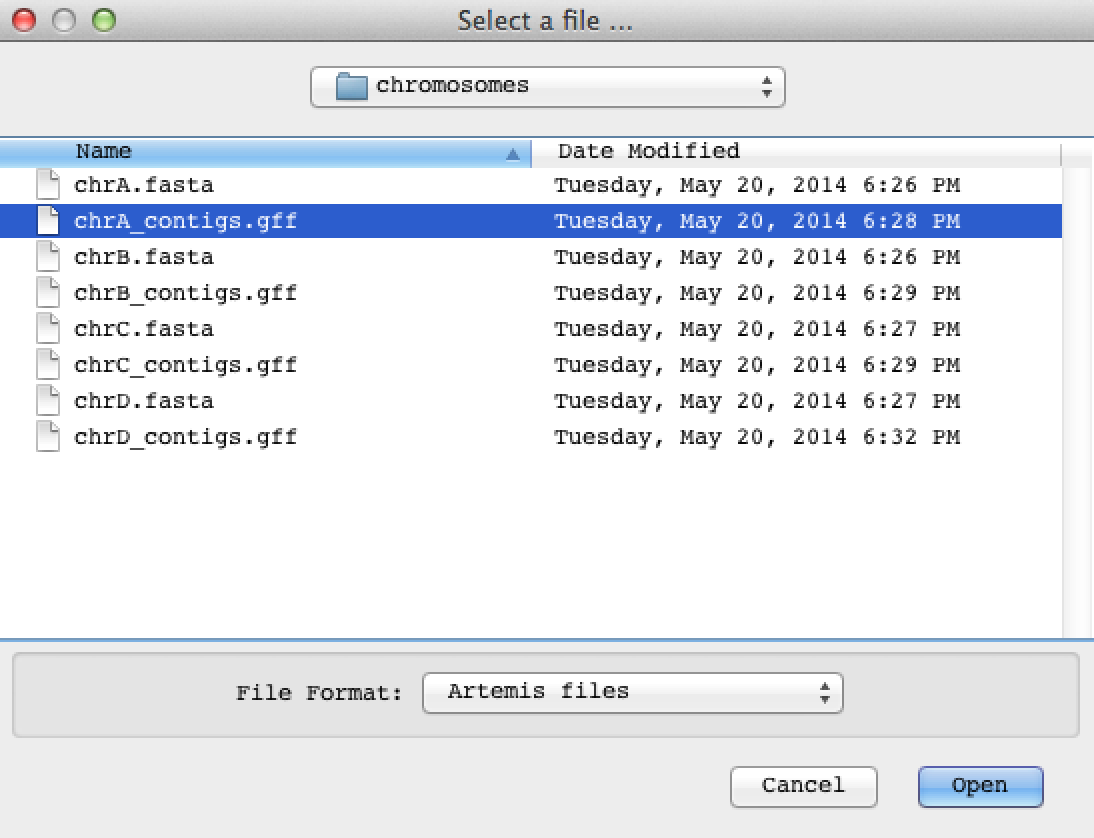
\includegraphics[width=0.7\textwidth]{images/artemis_select_contig_gff} 
    \end{center}
\end{frame}

  \begin{frame}
    \frametitle{Load the contig GFF}
    \begin{center}
      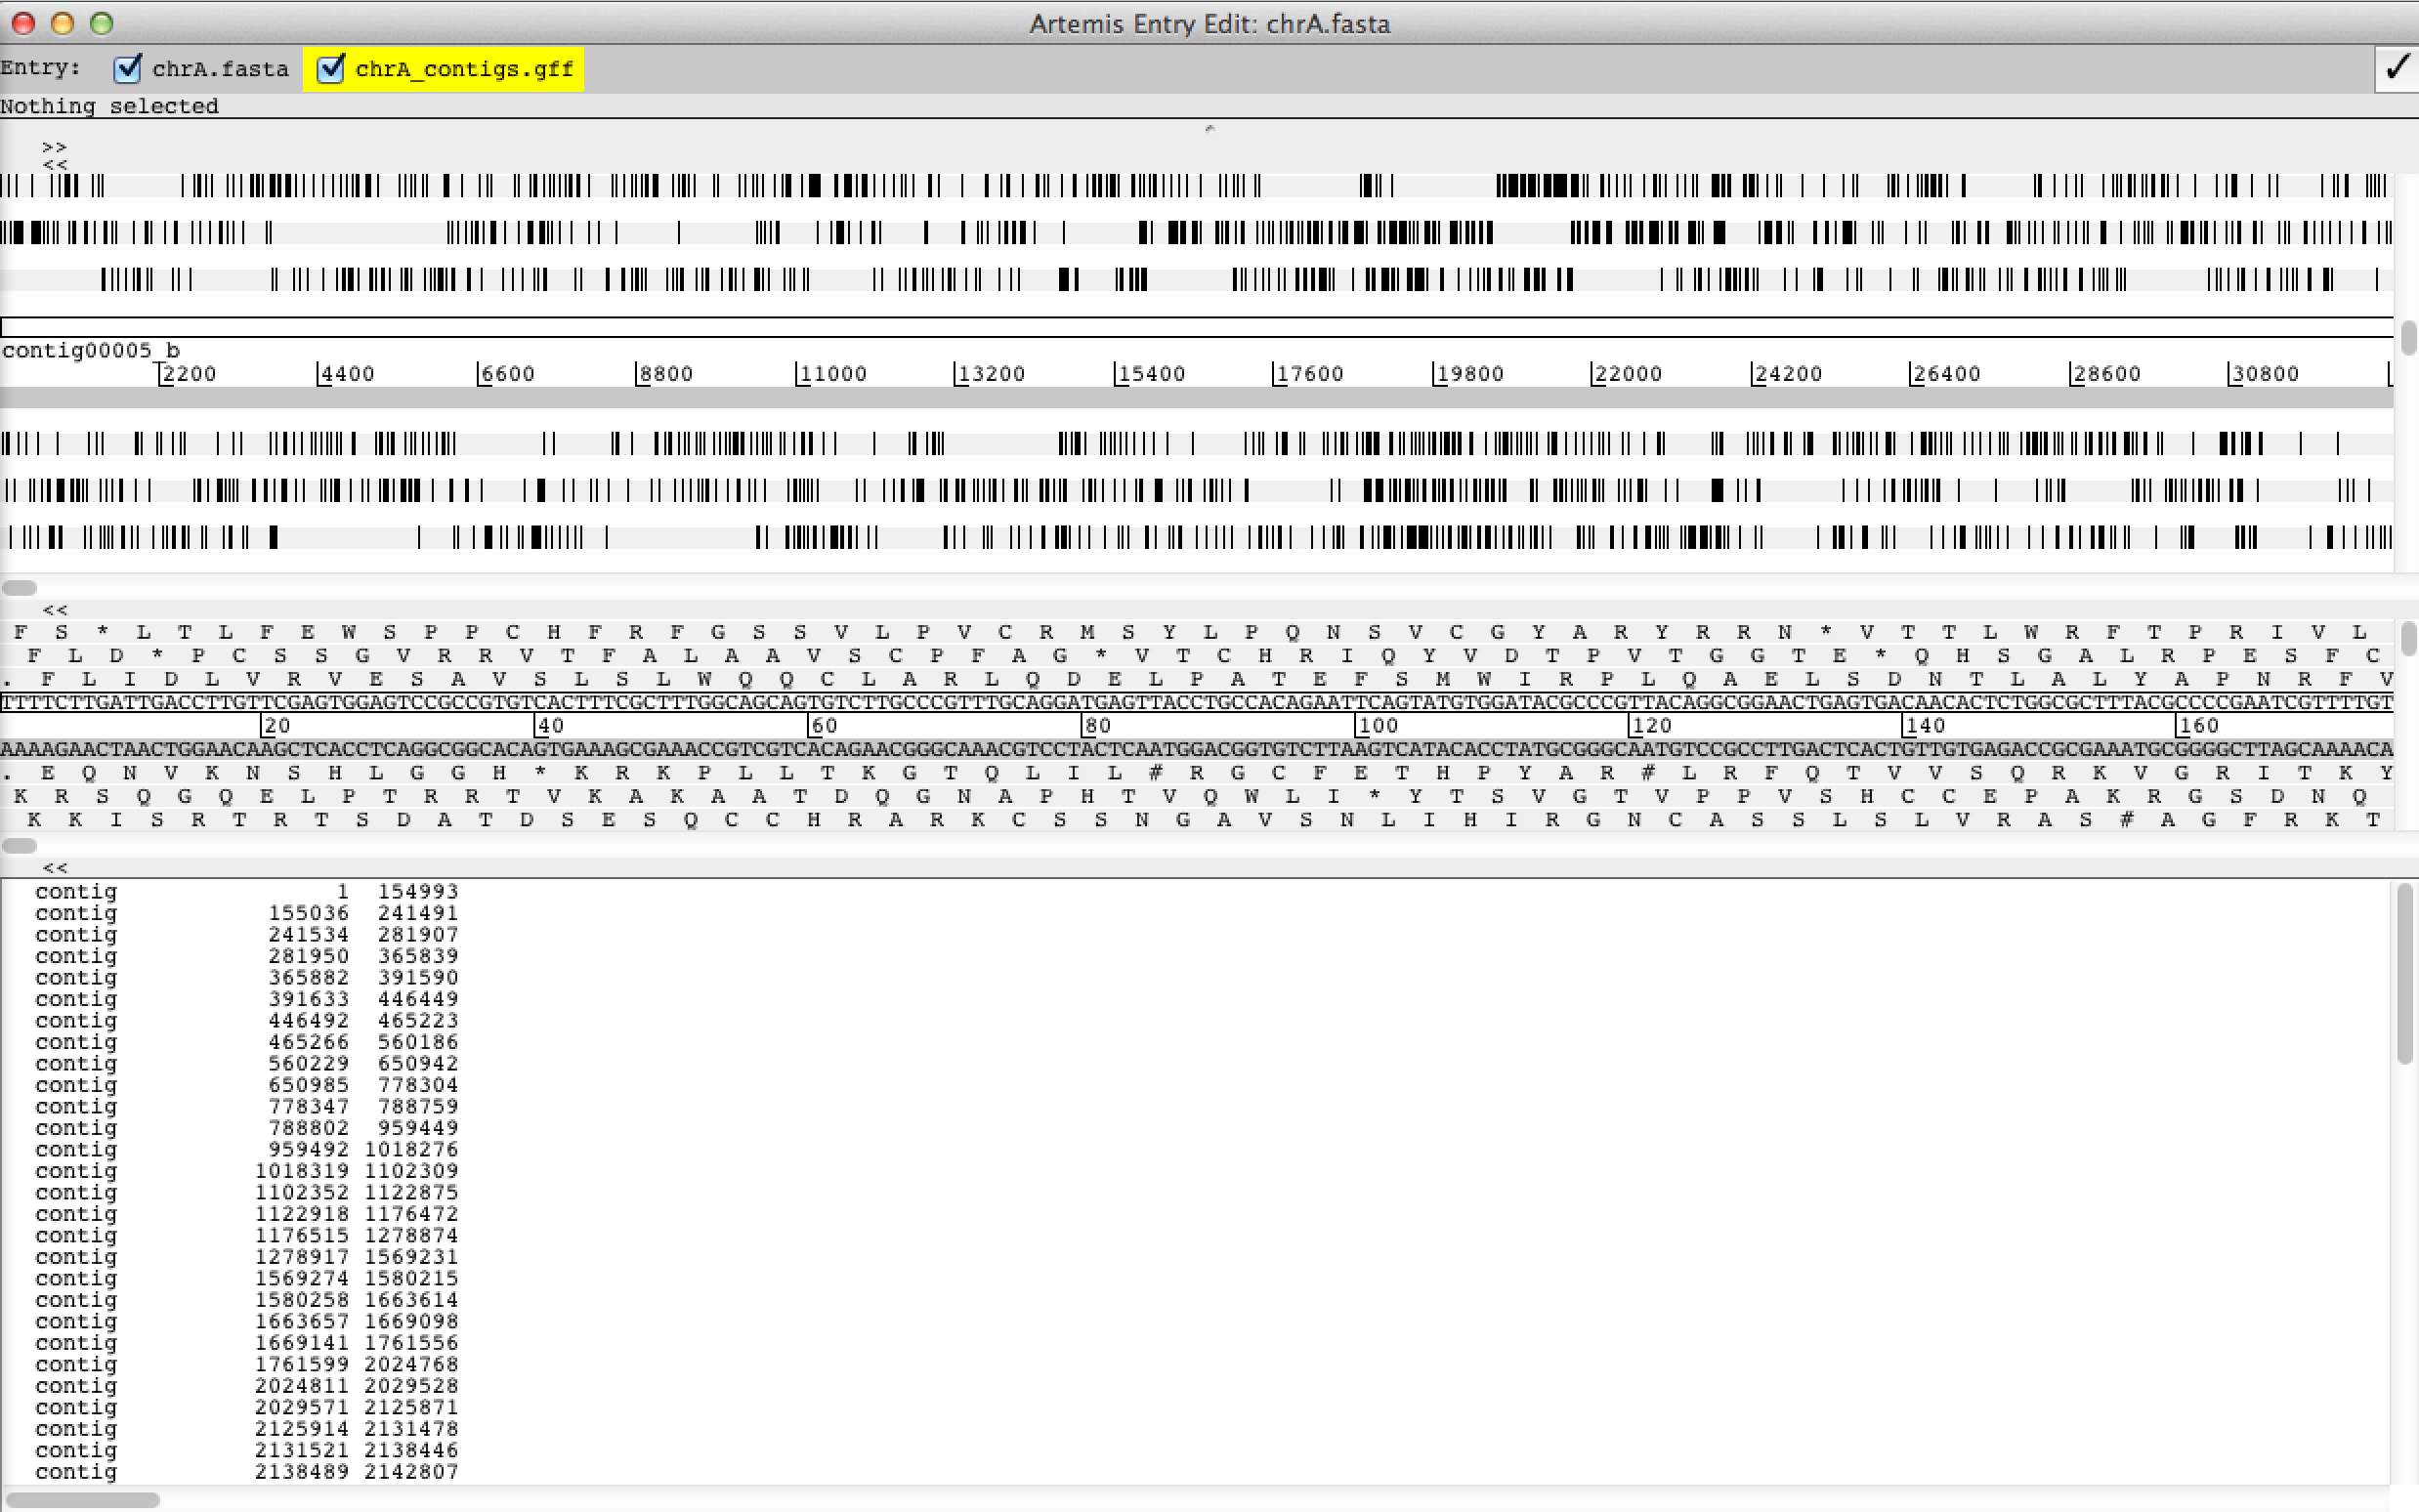
\includegraphics[width=0.9\textwidth]{images/artemis_loaded_contigs} 
    \end{center}
\end{frame}

  \begin{frame}
    \frametitle{Find the stitching sequence}
    The contigs are stitched with a specific sequence: see if you can find, and identify it.
    \begin{center}
      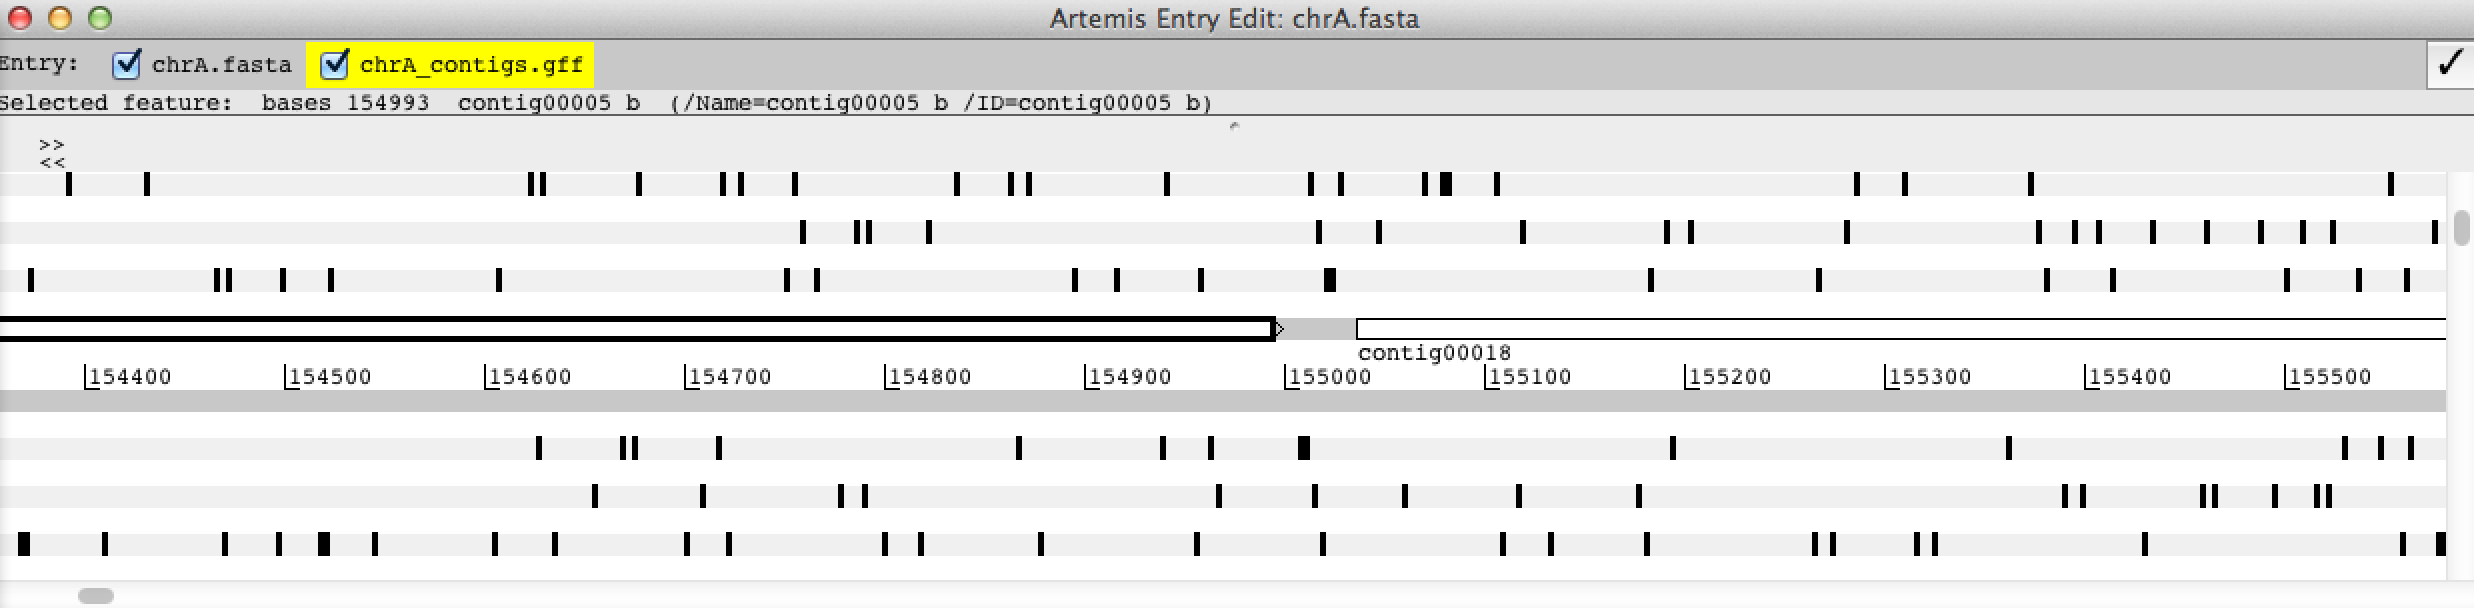
\includegraphics[width=\textwidth]{images/artemis_stitch_tease} 
    \end{center}
\end{frame}

  % ORF Prediction
  \section{Gene Prediction}
  \subsection{Intro}
    \begin{frame}
     \frametitle{Lines of Evidence}
     \begin{itemize}
       \item \textit{ab initio} genecalling: 
       \begin{itemize}
         \item Unsupervised methods - not trained on a dataset
         \item Supervised methods - trained on a dataset
       \end{itemize}
       \item homology matches
       \begin{itemize}
         \item alignment to genes from related organisms (annotation transfer)
         \item from known gene products (e.g. proteins, ncRNA)
         \item from transcripts/other intermediates (e.g. ESTs, cDNA, RNAseq)
       \end{itemize}
     \end{itemize}
    \end{frame}
    
    \begin{frame}
     \frametitle{Consensus Methods}
     \begin{itemize}
       \item Combine weighted evidence from multiple sources, using linear combination or graph theoretical methods
       \item For eukaryotes:
       \begin{itemize}
         \item EVM \url{http://evidencemodeler.sourceforge.net/}
         \item Jigsaw \url{http://www.cbcb.umd.edu/software/jigsaw/}
         \item GLEAN \url{http://sourceforge.net/projects/glean-gene/}
       \end{itemize}
     \end{itemize}
    \end{frame}
  
    \subsection{ORF Prediction}
    \begin{frame}
     \frametitle{ORF Prediction}
     \begin{itemize}
       \item Open Reading Frame = sequence between successive stop codons
       \item A very naive method - unsupervised \textit{de novo} prediction
       \item Sufficiently long ORFs are genes (or exons)
       \item Many tools:
       \begin{itemize}
         \item Artemis
         \item EMBOSS \texttt{getorf}
         \item hundreds of ``in-house'' scripts$\ldots$
       \end{itemize}
     \end{itemize}
    \end{frame}

    \begin{frame}
      \frametitle{ORF Prediction in Artemis}    
      \begin{center}
        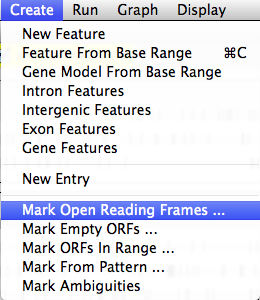
\includegraphics[width=0.4\textwidth]{images/artemis_orf0}     
      \end{center}
    \end{frame}

    \begin{frame}
      \frametitle{ORF Prediction in Artemis}
      Biological insight required: what size should the smallest ORF be?
      \begin{center}
        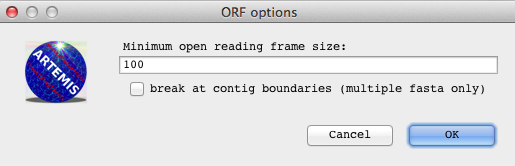
\includegraphics[width=0.9\textwidth]{images/artemis_orf1}     
      \end{center}
    \end{frame}

    \begin{frame}
      \frametitle{ORF Prediction in Artemis}    
      \begin{center}
        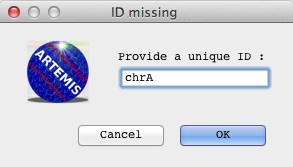
\includegraphics[width=0.9\textwidth]{images/artemis_orf2}     
      \end{center}
    \end{frame}

    \begin{frame}
      \frametitle{ORF Prediction in Artemis}    
      \begin{center}
        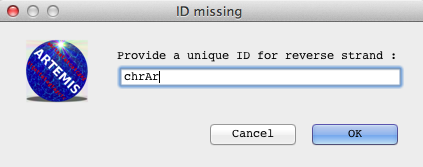
\includegraphics[width=0.9\textwidth]{images/artemis_orf3}     
      \end{center}
    \end{frame}

    \begin{frame}
      \frametitle{ORF Prediction in Artemis} 
      Is this good enough?
      \begin{center}
        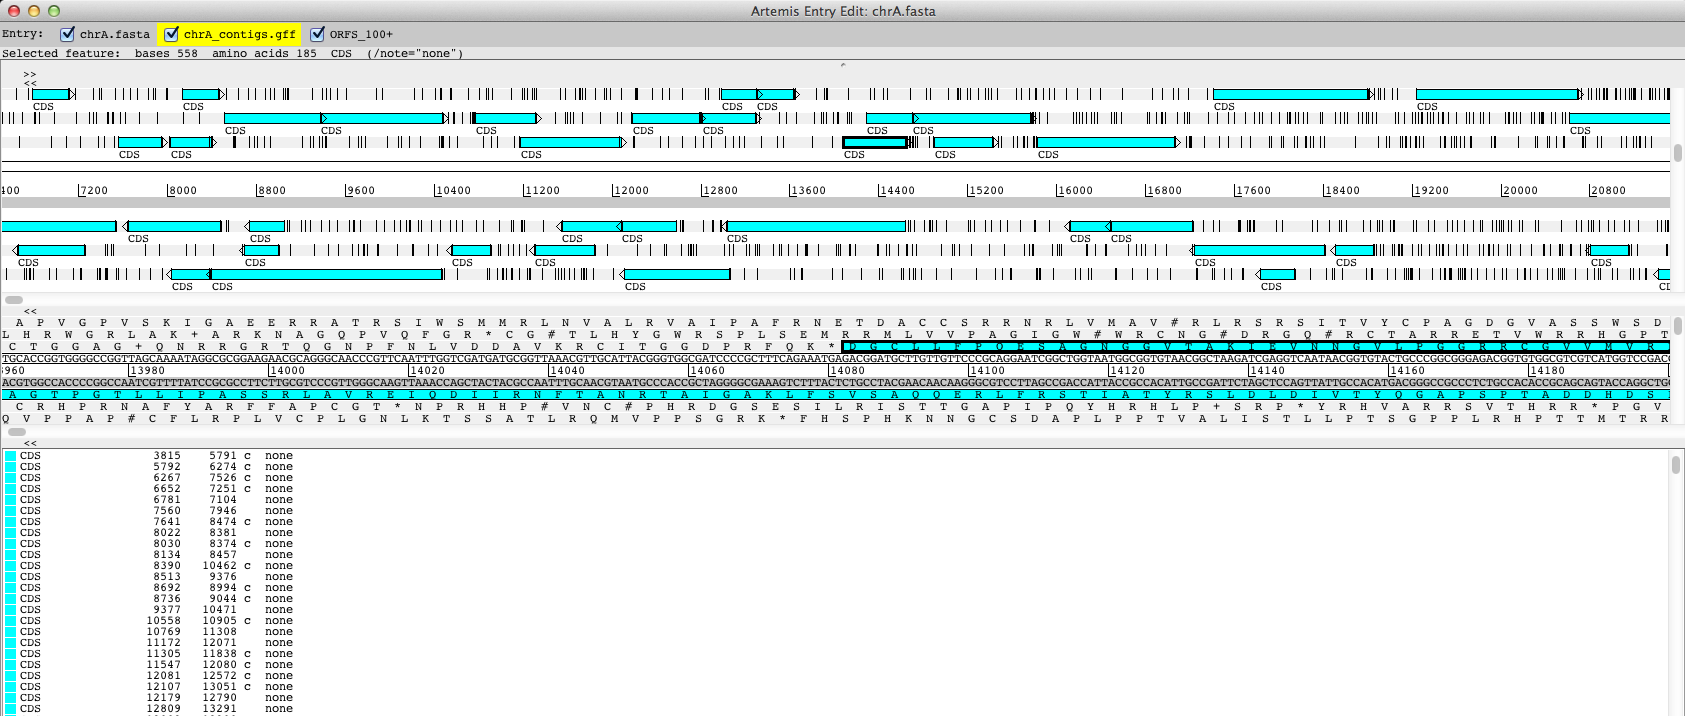
\includegraphics[width=0.9\textwidth]{images/artemis_orf4}     
      \end{center}
    \end{frame}

    \begin{frame}
      \frametitle{ORF Prediction in Artemis}    
      \begin{center}
        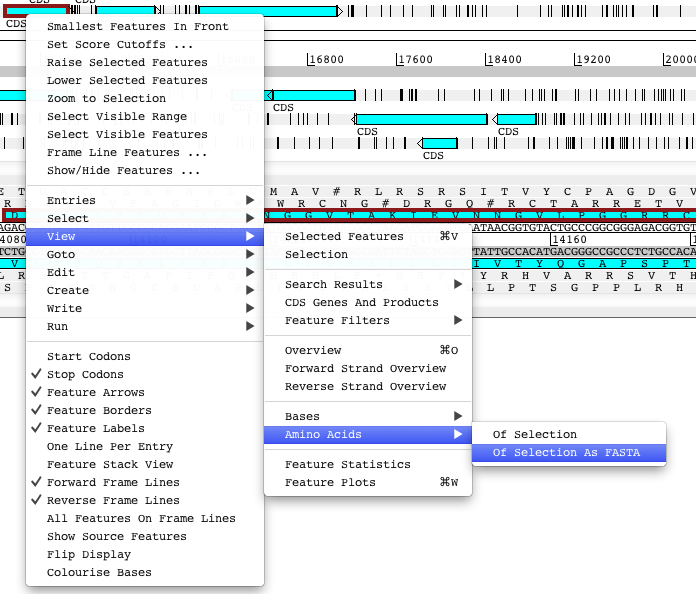
\includegraphics[width=0.7\textwidth]{images/artemis_orf5}     
      \end{center}
    \end{frame}

    \begin{frame}
      \frametitle{ORF Prediction in Artemis}
      Biological insight: CDS start with start codon.
      \begin{center}
        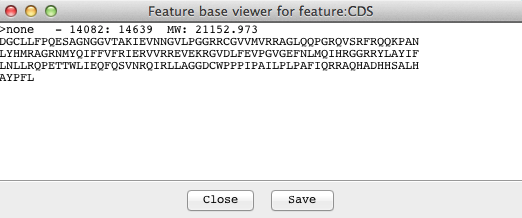
\includegraphics[width=0.9\textwidth]{images/artemis_orf6}     
      \end{center}
    \end{frame}

    \begin{frame}
      \frametitle{ORF Prediction in Artemis}    
      \begin{center}
        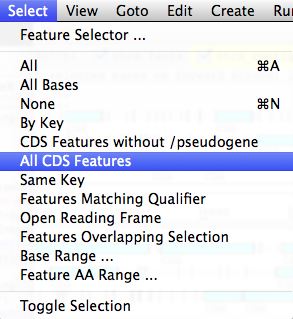
\includegraphics[width=0.5\textwidth]{images/artemis_orf7}     
      \end{center}
    \end{frame}

    \subsection{Trim Predictions, Recap}
    \begin{frame}
      \frametitle{ORF Prediction in Artemis}    
      \begin{center}
        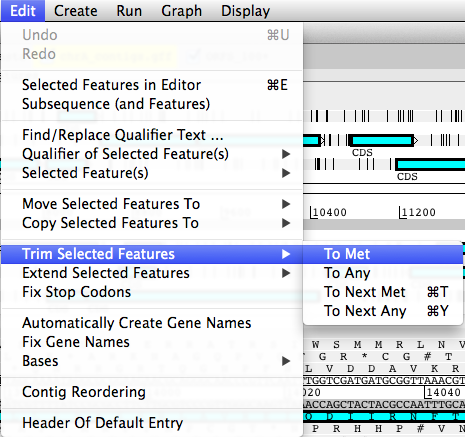
\includegraphics[width=0.6\textwidth]{images/artemis_orf8}     
      \end{center}
    \end{frame}

    \begin{frame}
      \frametitle{ORF Prediction in Artemis}
      What does this mean, in terms of biology?
      \begin{center}
        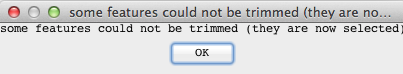
\includegraphics[width=0.9\textwidth]{images/artemis_orf9}     
      \end{center}
    \end{frame}

    \begin{frame}
      \frametitle{ORF Prediction in Artemis}    
      \begin{center}
        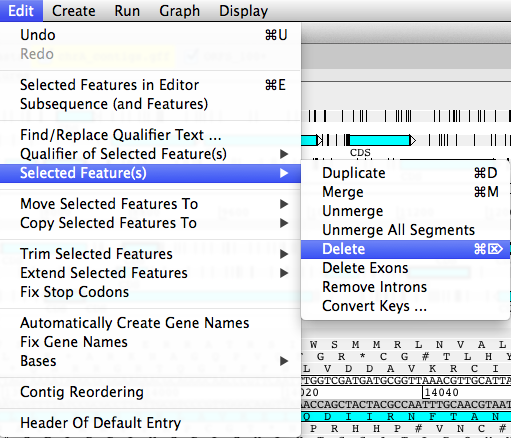
\includegraphics[width=0.6\textwidth]{images/artemis_orf10}     
      \end{center}
    \end{frame}

    \begin{frame}
      \frametitle{ORF Prediction in Artemis} 
      5410 ORFs with no start codon - how good is ORF detection at finding CDS?
      \begin{center}
        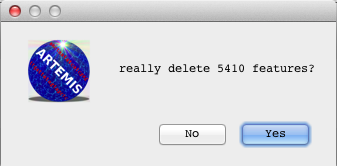
\includegraphics[width=0.9\textwidth]{images/artemis_orf11}     
      \end{center}
    \end{frame}

    \begin{frame}
      \frametitle{ORF Prediction in Artemis}
      Where do gene names come from?
      \begin{center}
        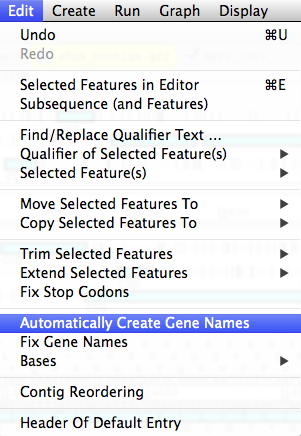
\includegraphics[width=0.3\textwidth]{images/artemis_orf12}     
      \end{center}
    \end{frame}

    \begin{frame}
      \frametitle{ORF Prediction in Artemis}    
      \begin{center}
        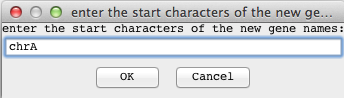
\includegraphics[width=0.9\textwidth]{images/artemis_orf13}     
      \end{center}
    \end{frame}

    \begin{frame}
      \frametitle{ORF Prediction in Artemis}   
      Is this good enough? 
      \begin{center}
        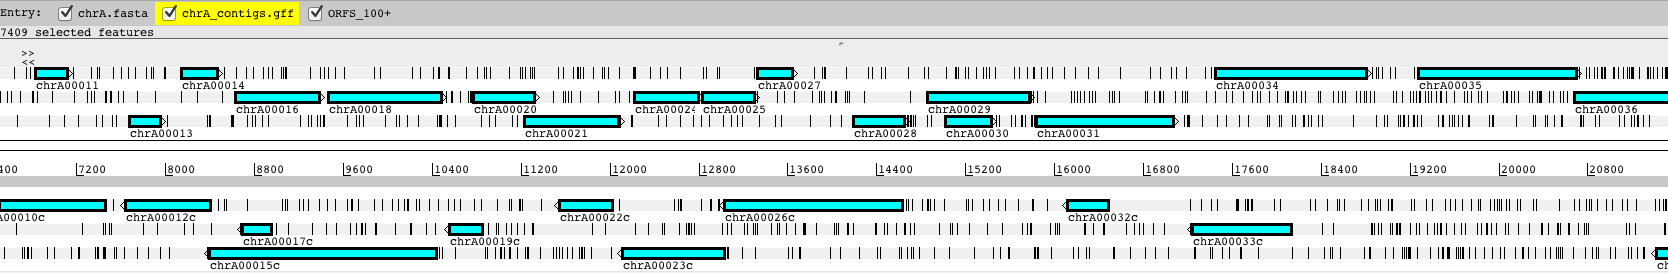
\includegraphics[width=0.9\textwidth]{images/artemis_orf14}     
      \end{center}
      Biological insight: do we expect CDS to overlap like this?
    \end{frame}

%\subsection{Recap}
\begin{frame}
    \frametitle{Basic Gene Finding}
    \begin{itemize}
      \item We just used Artemis to identify the longest coding region in each ORF, lots of manual steps
      \item This is the most basic gene finding, and can easily be automated, e.g. EMBOSS \texttt{getorf}
      \item Dedicated gene finders usually more appropriate...
    \end{itemize}
\end{frame}

\begin{frame}
    \frametitle{Finding Open Reading Frames (ORFs) within Artemis}
    \begin{itemize}
      \item<1-> ORF finding is naive, does not consider:
      \begin{itemize}
        \item Start codon
        \item Splicing
        \item Promoter/RBS motifs
        \item Wider context (e.g. overlapping genes)
      \end{itemize}
    \end{itemize}
\end{frame}

    \begin{frame}
      \frametitle{ORF Prediction in Artemis}   
      \framesubtitle{Lessons learned}   
      \begin{itemize}
        \item ORF finding is very simple, but still requires biological insight and parameter choices
        \item It's not a very precise way to identify genes or CDS (especially in eukaryotes)
        \item Even in prokaryotes, we only get a candidate set of CDS (many spurious) requiring manual refinement
      \end{itemize}
    \end{frame}

    \subsection{CDS Prediction}
    \begin{frame}
     \frametitle{Prokaryotic Prediction Methods}
     \begin{itemize}
       \item Prokaryotes ``easier'' than eukaryotes for gene prediction
       \begin{itemize}
         \item Very gene-dense (over 90\% of chromosome is coding sequence)
         \item No intron-exon structure
         \item Problem is essentially ``which possible ORF contains the true gene, and which start site is correct?''
         \item Still not a solved problem
       \end{itemize}       
     \end{itemize}
    \end{frame}

    \begin{frame}
     \frametitle{Two \textit{ab initio} Prokaryotic Prediction Methods}
     You will be using two tools
     \begin{itemize}
       \item Glimmer
       \begin{itemize}
         \item Interpolated Markov models
         \item Can be trained on ``gold standard'' datasets
       \end{itemize}
       \item Prodigal
       \begin{itemize}
         \item Log-likelihood model based on GC frame plots, followed by dynamic programming
         \item Can be trained on ``gold standard'' datasets
       \end{itemize}
     \end{itemize}
    \end{frame}

% [fragile] frames must end with \end{frame} directly following a newline, or they break!
\begin{frame}[fragile]
\frametitle{Using Glimmer}
Supervised - we train on a related complete genome sequence, then run \texttt{glimmer3}
\begin{lstlisting}[language=bash]
$ wget ftp://ftp.ncbi.nih.gov/genomes/Bacteria/Pectobacterium_atrosepticum_SCRI1043_uid57957/NC_004547.ffn
$ build-icm -r NC_004547.icm < NC_004547.ffn
$ glimmer3 -o 50 -g 110 -t 30 chrA.fasta NC_004547.icm chrA_glimmer3
\end{lstlisting}
    \begin{itemize}
      \item \texttt{-o 50}: max overlap bases
      \item \texttt{-g 110}: min gene length
      \item \texttt{-t 30}:  threshold score
    \end{itemize}
\end{frame}

\begin{frame}[fragile]
\frametitle{Using Glimmer}
\texttt{glimmer3} output is not standard GFF format:
\begin{lstlisting}[language=bash]
$ head -n 4 chrA_glimmer3.predict 
>chrA
orf00001       36     1430  +3     8.81
orf00002     1435     2535  +1    11.51
orf00005     2676     3761  +3     8.63
\end{lstlisting}
We could Google for help, or use provided conversion script:
\begin{lstlisting}[language=bash]
$ python glimmer_to_gff.py chrA_glimmer3.predict
\end{lstlisting}    
\end{frame}

\begin{frame}[fragile]
\frametitle{Using Glimmer}
We now have output in GFF
\begin{lstlisting}[language=bash]
$ head -n 3 chrA_glimmer3.gff 
chrA	Glimmer	CDS	36	1430	8.81	+	0	ID=orf00001;Name=orf00001
chrA	Glimmer	CDS	1435	2535	11.51	+	0	ID=orf00002;Name=orf00002
chrA	Glimmer	CDS	2676	3761	8.63	+	0	ID=orf00005;Name=orf00005
\end{lstlisting}
\end{frame}

% [fragile] frames must end with \end{frame} directly following a newline, or they break!
\begin{frame}[fragile]
\frametitle{Using Prodigal}
Unsupervised (i.e. untrained) mode
\begin{lstlisting}[language=bash]
$ prodigal -f gff -o chrA_prodigal.gff -i chrA.fasta
\end{lstlisting}
\end{frame}

% [fragile] frames must end with \end{frame} directly following a newline, or they break!
\begin{frame}[fragile]
\frametitle{Using Prodigal}
Prodigal GFF output is correctly formatted and informative
\begin{lstlisting}[language=]
$ head -n 6 chrA_prodigal.gff 
##gff-version  3
# Sequence Data: seqnum=1;seqlen=4727782;seqhdr="chrA"
# Model Data: version=Prodigal.v2.50;run_type=Single;model="Ab initio";gc_cont=54.48;transl_table=11;uses_sd=1
chrA	Prodigal_v2.50	CDS	3	1430	188.5	+	0	ID=1_1;partial=10;start_type=Edge;rbs_motif=None;rbs_spacer=None;score=188.54;cscore=185.37;sscore=3.18;rscore=0.00;uscore=3.18;tscore=0.00
chrA	Prodigal_v2.50	CDS	1435	2535	185.6	+	0	ID=1_2;partial=00;start_type=ATG;rbs_motif=None;rbs_spacer=None;score=185.61;cscore=184.24;sscore=1.36;rscore=-7.73;uscore=3.48;tscore=4.37
chrA	Prodigal_v2.50	CDS	2676	3761	146.2	+	0	ID=1_3;partial=00;start_type=ATG;rbs_motif=None;rbs_spacer=None;score=146.19;cscore=149.82;sscore=-3.63;rscore=-7.73;uscore=-0.28;tscore=4.37
\end{lstlisting}
\end{frame}

    \begin{frame}
     \frametitle{Comparing predictions in Artemis}
      \begin{center}
        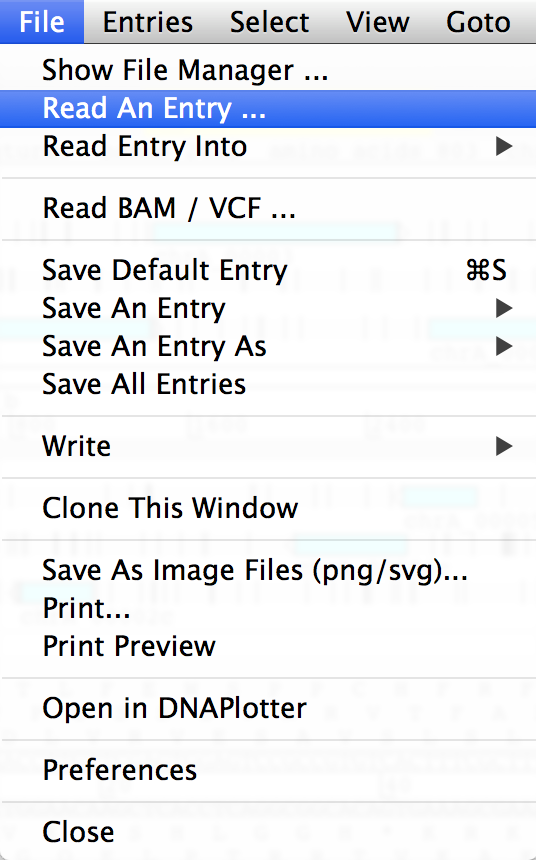
\includegraphics[width=0.3\textwidth]{images/artemis_cdspred0}     
      \end{center}
    \end{frame}

    \begin{frame}
     \frametitle{Comparing predictions in Artemis}
      \begin{center}
        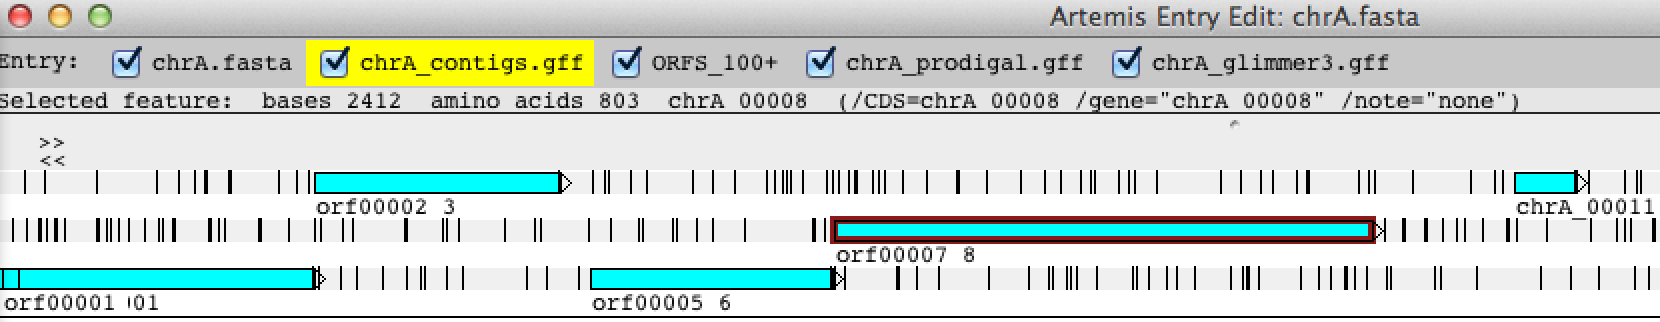
\includegraphics[width=0.9\textwidth]{images/artemis_cdspred1}     
      \end{center}
    \end{frame}

    \begin{frame}
     \frametitle{Comparing predictions in Artemis}
      \begin{center}
        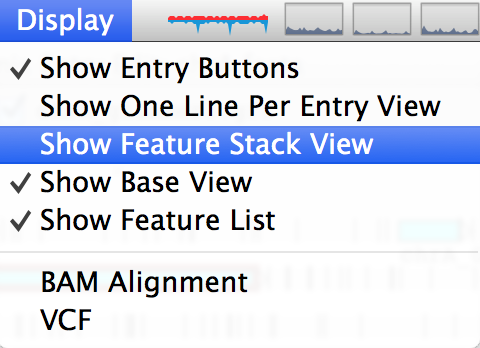
\includegraphics[width=0.4\textwidth]{images/artemis_cdspred2}     
      \end{center}
    \end{frame}

    \begin{frame}
     \frametitle{Comparing predictions in Artemis}
     %TODO - How to set the colours for each set of predictions?
     Do ORF(orange)/CDS(green,blue) prediction methods agree?
      \begin{center}
        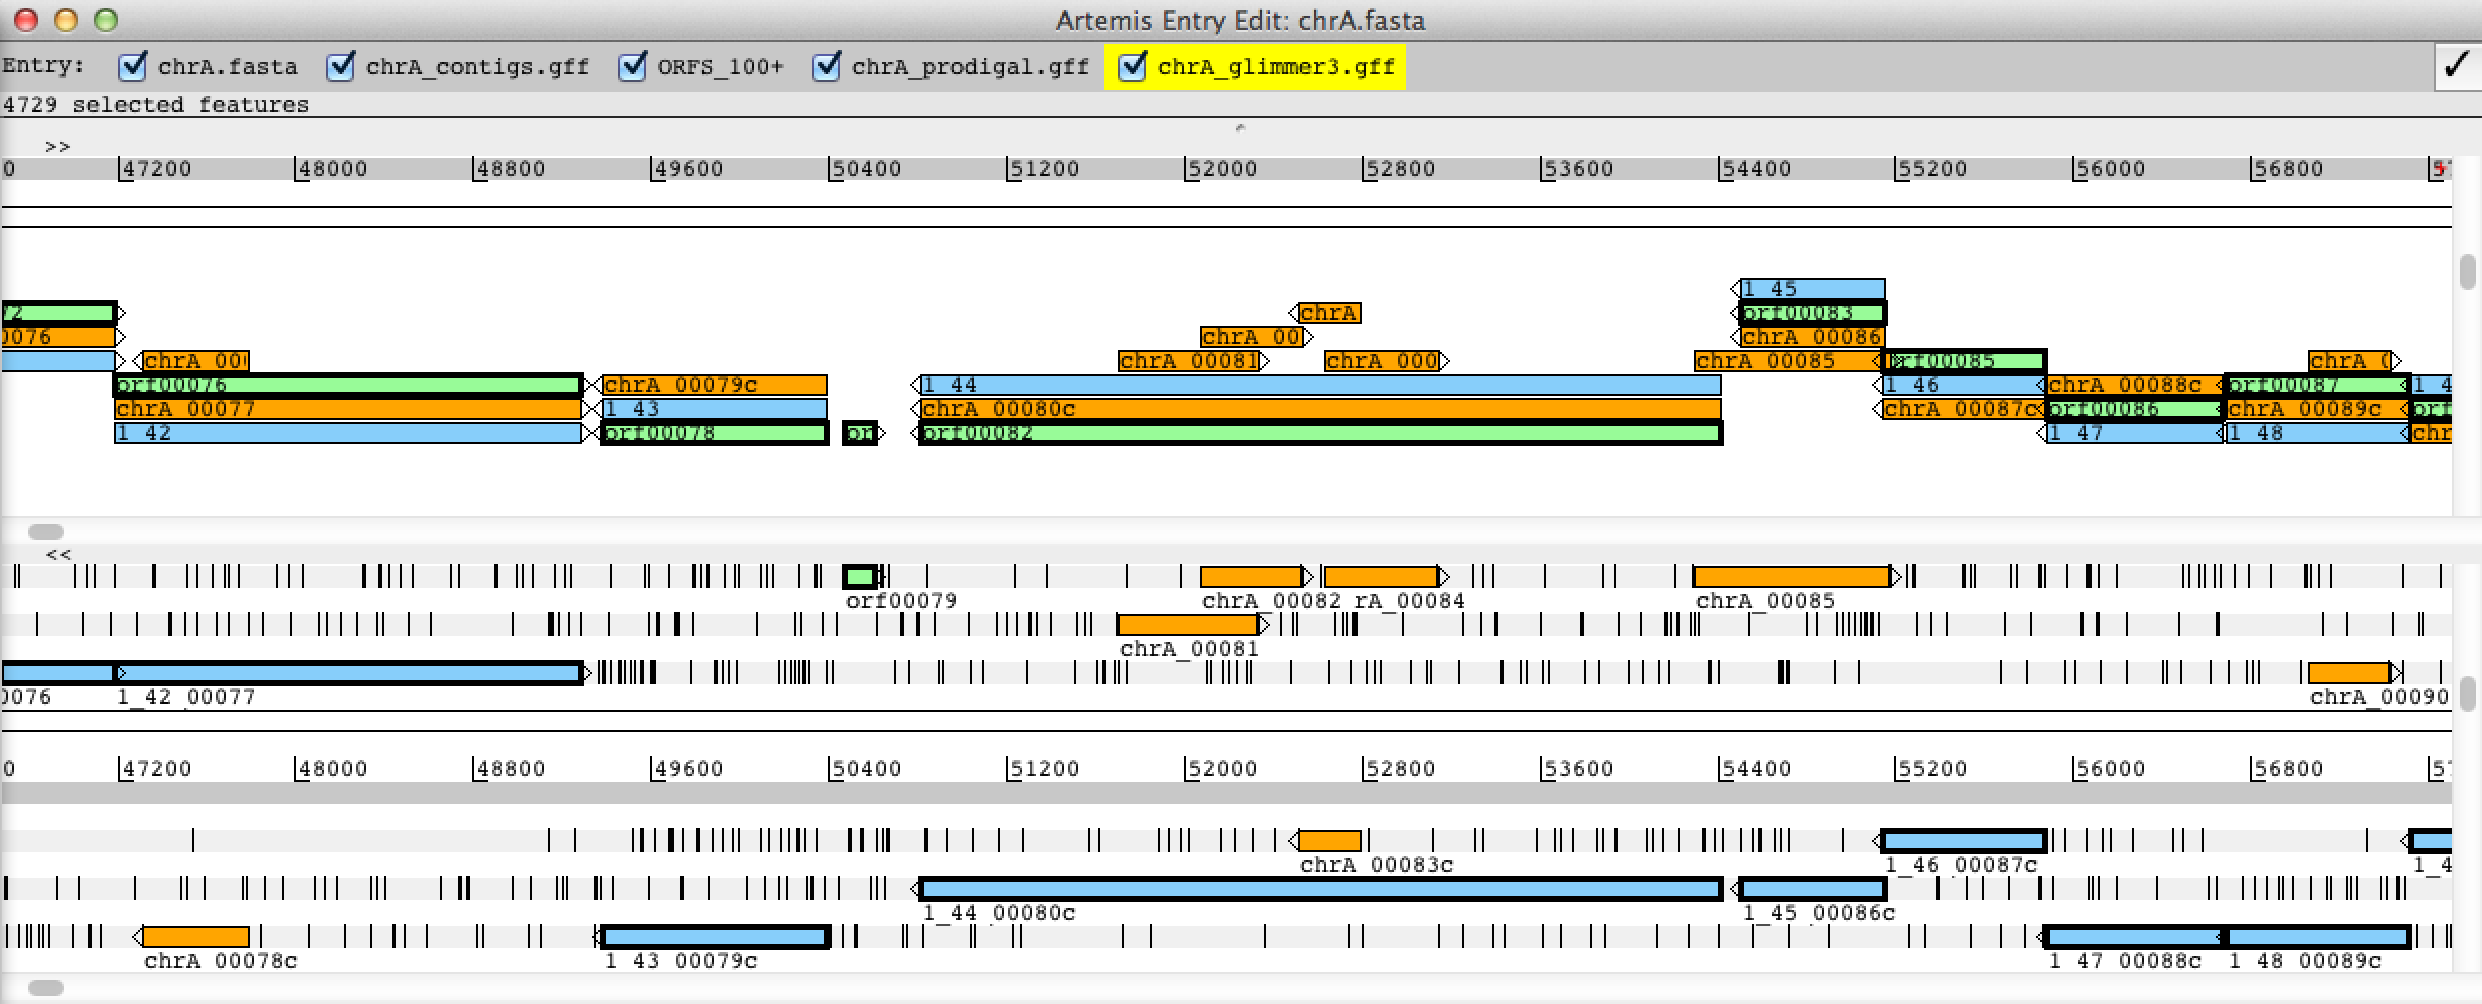
\includegraphics[width=0.9\textwidth]{images/artemis_cdspred3}     
      \end{center}
    \end{frame}

    \begin{frame}
     \frametitle{Comparing predictions in Artemis}
     Do \texttt{glimmer}(green)/\texttt{prodigal}(blue) CDS prediction methods agree?
      \begin{center}
        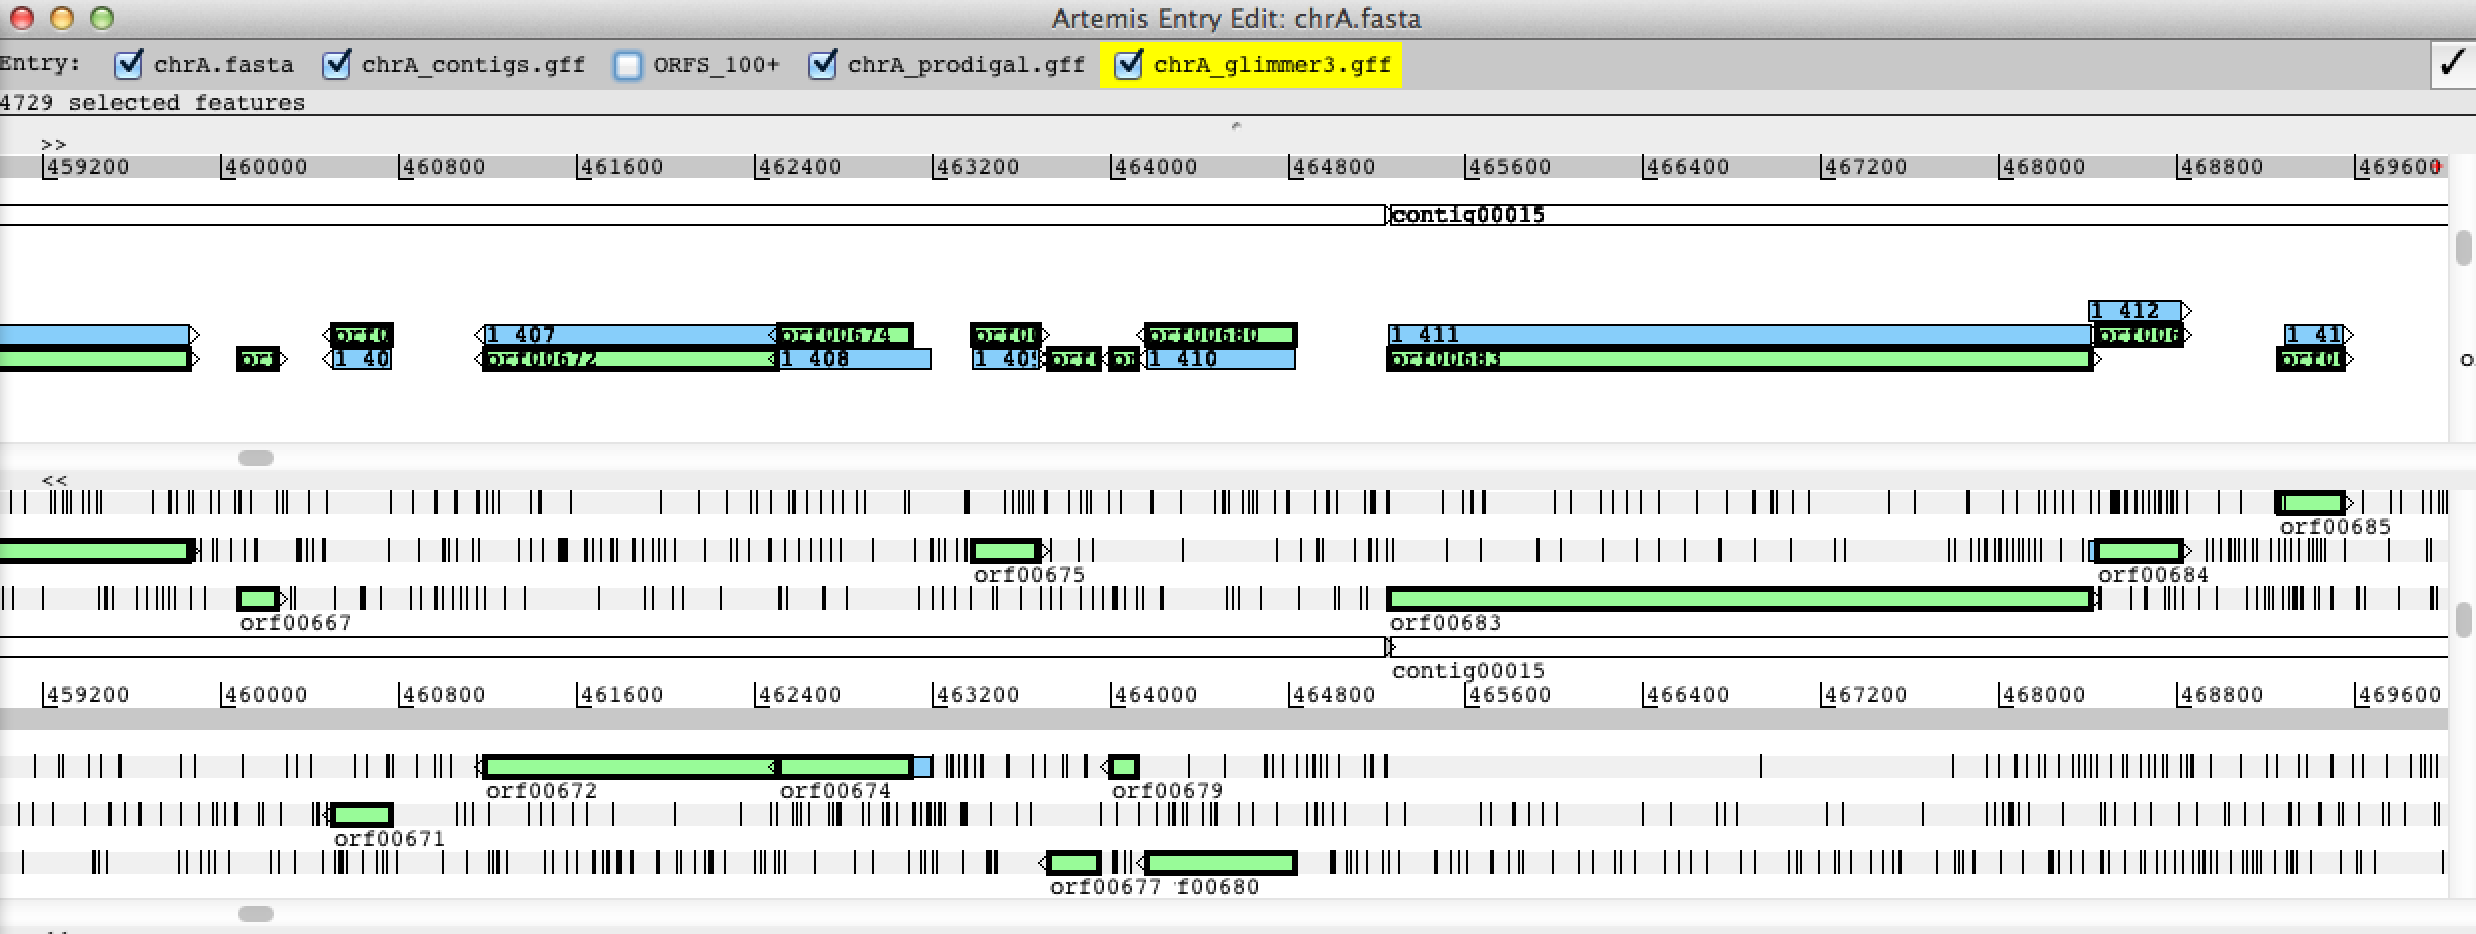
\includegraphics[width=0.9\textwidth]{images/artemis_cdspred4}     
      \end{center}
      How do we know which is best?
    \end{frame}

    \subsection{Assessing Prediction Methods}
    \begin{frame}
     \frametitle{Using a ``Gold Standard''}
     A general approach for \emph{all} predictive methods
     \begin{itemize}
       \item Define a known, ``correct'' set of true/false, positive/negative etc. examples - the ``gold standard''
       \item Evaluate your predictive method against that set for
       \begin{itemize}
         \item sensitivity, specificity, accuracy, precision, etc.
       \end{itemize}
     \end{itemize}
     Many methods available, coverage beyond the scope of this introduction
   \end{frame}

  \begin{frame}
    \frametitle{Contingency Tables}
    \begin{center}
	\begin{tabular}{cc|c|c|}
	  \cline{3-4}
		& & \multicolumn{2}{|c|}{Condition (Gold standard)}\\
	  \cline{3-4}
		& & True & False \\
	  \hline
	  \multicolumn{1}{ |c| }{\multirow{2}{*}{Test outcome}}& 
	  \multicolumn{1}{ |c| }{Positive} & True Positive \cellcolor{green} & 
	    False Positive\cellcolor{red}\\
	  \cline{2-4}
	  \multicolumn{1}{ |c| }{} & \multicolumn{1}{ |c| }{Negative} & 
	    False Negative\cellcolor{red} & True Negative \cellcolor{green}\\
	  \hline
	\end{tabular}
	\end{center}
	Sensitivity = TPR = $TP/(TP + FN)$ \\
	Specificity = TNR = $TN/(FP + TN)$ \\
	FPR = $1-\text{Specificity} = FP/(FP + TN)$ \\
	If you don't have this information, you can't interpret predictive results properly.
\end{frame}

    \begin{frame}
     \frametitle{Why Performance Metrics Matter}
     \begin{itemize}
       \item<1-> You go for a checkup, and are tested for disease $X$
       \item<1-> The test has $\text{sensitivity}=0.95$ (predicts disease where there is disease)
       \item<1-> The test has $\text{FPR}=0.01$ (predicts disease where there is no disease)
       \item<2-> Your test is \emph{positive}
       \item<2-> What is the probability that you have disease $X$?
       \begin{itemize}
         \item 0.01, 0.05, 0.50, 0.95, 0.99?
       \end{itemize}
     \end{itemize} 
   \end{frame}

    \begin{frame}
     \frametitle{Why Performance Metrics Matter}
     \begin{itemize}
       \item<1-> What is the probability that you have disease $X$?
       \item<1-> Unless you know the \emph{baseline occurrence} of disease $X$, you cannot know.
       \item<2-> Baseline occurrence: $f_X$
       \begin{itemize}
         \item $f_X = 0.01 \implies P(\text{disease}|\text{+ve}) = 0.490 \approx 0.5$
         \item $f_X = 0.8 \implies P(\text{disease}|\text{+ve}) = 0.997 \approx 1.0$         
       \end{itemize}
     \end{itemize} 
   \end{frame}

    \begin{frame}
     \frametitle{Why Performance Metrics Matter}
     \begin{itemize}
       \item<1-> Imagine a predictor for protein functional class
       \item<1-> Predictor has has $\text{sensitivity}=0.95$, $\text{FPR}=0.01$
       \item<1-> You run the predictor on 20,000 proteins in an organism
       \item<2-> We estimate $\approx$ 200 members in protein complement, so $f_X=0.01$
       \begin{itemize}
         \item $f_X = 0.01 \implies P(\text{disease}|\text{+ve}) = 0.490 \approx 0.5$
       \end{itemize}
     \end{itemize} 
   \end{frame}

    \begin{frame}
     \frametitle{Bayes' Theorem}
     \begin{itemize}
       \item May seem counter-intuitive: 95\% sensitivity, 99\% specificity $\implies$ 50\% chance of any prediction being incorrect
       \item Probability given by Bayes' Theorem
       \begin{itemize}
         \item $P(X|+) =  \frac{P(+|X) P(X)}{P(+|X) P(X) + P(+|\bar{X}) P(\bar{X})}$
       \end{itemize}
       \item This is commonly overlooked in the literature (confirmation bias?)
       \item e.g. in paper describing novel TTSS predictor: \\
         ``The surprisingly high number of (false) positives in genomes without TTSS exceeds the expected false positive rate"
     \end{itemize} 
   \end{frame}

    \begin{frame}
     \frametitle{Interpreting Performance Metrics}
     \begin{itemize}
       \item<1-> Use Bayes' Theorem!
       \item<1-> Predictions apply to groups, not individual members of the group. e.g.
       \begin{itemize}
         \item Test for airport smugglers has $P(\text{smuggler}|+) = 0.9$
         \item Test gives 100 positives
       \end{itemize}
       \item<1-> Which specific individuals are truly smugglers?
       \item<2-> The test \emph{does not} allow you to determine this - you need more evidence for each individual
       \item<2->  Same principle applies to all other tests, (including protein functional class prediction) - you should not `cherry-pick' for publication without other evidence
     \end{itemize} 
   \end{frame}

    \begin{frame}
     \frametitle{``Gold Standard'' results}
     \begin{itemize}
       \item Tested \texttt{glimmer} and \texttt{prodigal} on two "gold standards"
       \begin{itemize}
         \item Manually annotated ($>$3 expert person years) close relative
         \item Community-annotated close relative
       \end{itemize}
       \item Both methods trained directly on the annotated genes in each organism!
     \end{itemize} 
   \end{frame}

    \begin{frame}
     \frametitle{``Gold Standard'' results}
     \framesubtitle{Manually annotated: 4550 CDS}
    \begin{center}
	\begin{tabular}{r|l|l}
	  genecaller & \texttt{glimmer} & \texttt{prodigal}  \\
	  \hline
	  predicted & 4752    & 4287  \\
	  missed & 284 (6\%)   & 407 (9\%)  \\
	  \hline
	  \emph{Exact Prediction} & & \\
  	  sensitivity   & 62\%   & 71\%  \\
  	  FDR   & 41\%   & 25\%  \\  
	  PPV   & 59\% & 75\%  \\  
	  \hline
	  \emph{Correct ORF} & & \\
  	  sensitivity   & 94\%   & 91\% \\
  	  FDR   & 10\%  & 3\% \\  
	  PPV   & 90\% & 97\%  \\  
	\end{tabular}
	\end{center}     
   \end{frame}

    \begin{frame}
     \frametitle{``Gold Standard'' results}
     \framesubtitle{Community annotated: 4475 CDS}
    \begin{center}
	\begin{tabular}{r|l|l}
	  genecaller & \texttt{glimmer} & \texttt{prodigal}  \\
	  \hline
	  predicted & 4679    & 4467  \\
	  missed & 112 (3\%)   & 156 (3\%)  \\
	  \hline
	  \emph{Exact Prediction} & & \\
  	  sensitivity   & 62\%   & 86\%  \\
  	  FDR   & 31\%   & 14\%  \\  
	  PPV   & 69\% & 86\%  \\  
	  \hline
	  \emph{Correct ORF} & & \\
  	  sensitivity   & 97\%   & 97\% \\
  	  FDR   & 7\%  & 3\% \\  
	  PPV   & 93\% & 97\%  \\  
	\end{tabular}
	\end{center}     
   \end{frame}

    \begin{frame}
      \frametitle{Gene/CDS Prediction}   
      \framesubtitle{Lessons learned}   
      \begin{itemize}
        \item Many alternative methods, all perform differently (not necessarily concordant)
        \item To assess/choose methods, performance metrics are required
        \item Even on (relatively simple) prokaryotes, current best methods imperfect
        \item Manual assessment and intervention is essential, and the longest part of the process
      \end{itemize}
    \end{frame}
    
    
% Whole genome comparisons
\section{Genome Alignments}
  \subsection{BLAST comparisons}
% [fragile] frames must end with \end{frame} directly following a newline, or they break!
  \begin{frame}[fragile]
    \frametitle{Run a megaBLAST Comparison}
    BLAST your chromosome against the comparator sequence. \\
    Put results in \texttt{chrA\_megablast\_Pba.tab}
\begin{lstlisting}[language=bash]
$ blastn -query chrA.fasta -subject NC_004547.fna -out chrA_megablast_Pba.tab -outfmt 6 
$ head -n 3 chrA_megablast_Pba.tab 
chrA	gi|50118965|ref|NC_004547.2|:10948-12453	80.34	1511	287	10	4579450	4580955	1506	1	0.0	1136
chrA	gi|50118965|ref|NC_004547.2|:c33859-32447	82.04	1409	253	0	4563151	4564559	1	1409	0.0	1201
chrA	gi|50118965|ref|NC_004547.2|:c34917-33868	82.48	1050	184	0	4562093	4563142	1	1050	0.0	 920
\end{lstlisting}
Note this defaults to using MEGABLAST...
\end{frame}
    
% [fragile] frames must end with \end{frame} directly following a newline, or they break!
  \begin{frame}[fragile]
    \frametitle{Run a BLASTN Comparison}
    BLAST your chromosome against the comparator sequence \\
    Put results in \texttt{chrA\_blastn\_Pba.tab}
\begin{lstlisting}[language=bash]
$ blastn -query chrA.fasta -subject NC_004547.fna -out chrA_blastn_Pba.tab -outfmt 6 -task blastn
$ head -n 3 chrA_blastn_Pba.tab 
chrA	gi|50118965|ref|NC_004547.2|:5629-7497	79.68	1865	379	0	4584915	4586779	1865	1	0.0	1654
chrA	gi|50118965|ref|NC_004547.2|:5629-7497	92.59	27	2	0	4479367	4479393	1254	1280	0.004	41.0
chrA	gi|50118965|ref|NC_004547.2|:5629-7497	100.00	17	0	0	4613022	4613038	52	36	2.1	31.9
\end{lstlisting}
Note note we added \texttt{-task blastn}
\end{frame}
    
% [fragile] frames must end with \end{frame} directly following a newline, or they break!
  \begin{frame}[fragile]
    \frametitle{Do BLASTN and megaBLAST comparisons agree?}
    Check the number of alignments returned with \texttt{wc}
\begin{lstlisting}[language=bash]
$ wc chrA_megablast_Pba.tab 
    2675   32100  242539 chrA_megablast_Pba.tab
$ wc chrA_blastn_Pba.tab
   31792  381504 2850953 chrA_blastn_Pba.tab
\end{lstlisting}
    What is this telling us? \\
    Why do the results differ?
\end{frame}

  \begin{frame}
    \frametitle{BLASTN vs megaBLAST}
    \begin{itemize}
      \item<1-> BLASTN uses the BLAST algorithm, megaBLAST does not
      \begin{itemize}
        \item (though BLAST+ BLASTN now uses megaBLAST by default)
      \end{itemize}      
      \item<1-> megaBLAST uses a fast, greedy algorithm due to Zhang et al. (2000) \url{http://www.ncbi.nlm.nih.gov/pubmed/10890397}
      \item<2-> megaBLAST is optimised for
      \begin{itemize}
        \item genome-level searches
        \item queries on large sequence sets (automatic query packing)
        \item long alignments of similar sequences, with SNPs/sequencing errors
      \end{itemize}
      \item<2-> A discontinuous mode (dc-megaBLAST) is recommended for more divergent sequences
    \end{itemize}
\end{frame}

\begin{frame}[fragile]
\frametitle{Viewing alignments in ACT}
Start ACT from the command line:
\begin{lstlisting}[language=bash]
$ act &
\end{lstlisting}
      \begin{center}
        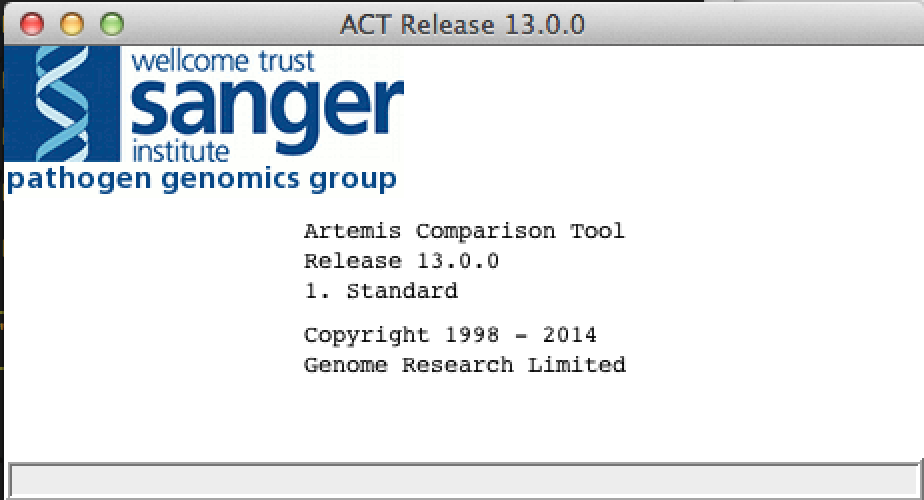
\includegraphics[width=0.6\textwidth]{images/act_wgs1}
      \end{center}
\end{frame}

    \begin{frame}
      \frametitle{Viewing alignments in ACT}
       Use the ``File'', ``Open...'' menu item:
      \begin{center}
        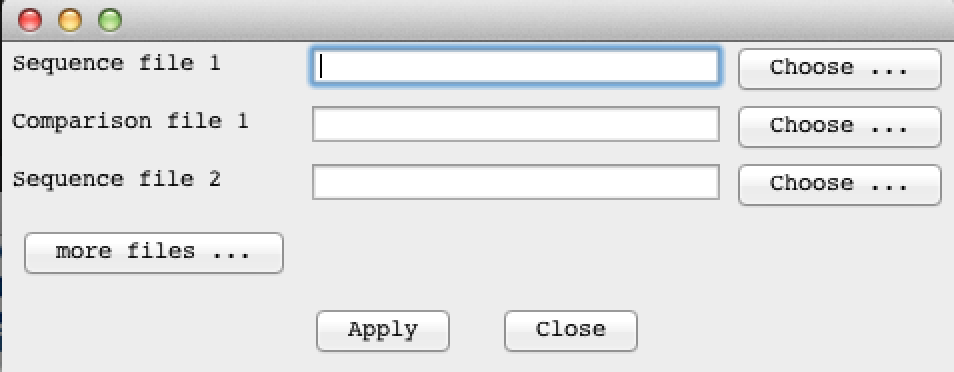
\includegraphics[width=0.9\textwidth]{images/act_wgs2}
      \end{center}
    \end{frame}

    \begin{frame}
      \frametitle{Viewing alignments in ACT}
      Use \texttt{more files ...} to increase the number of comparisons
      \begin{center}
        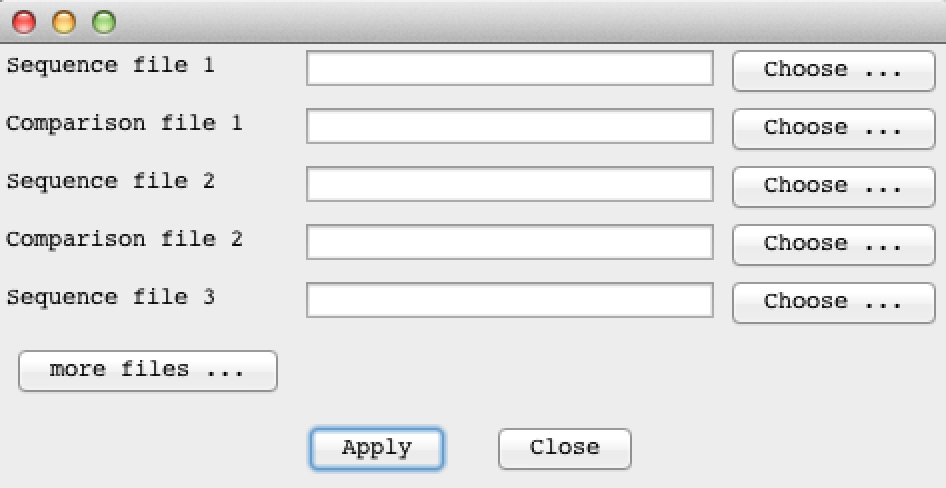
\includegraphics[width=0.9\textwidth]{images/act_wgs3}
      \end{center}
    \end{frame}

    \begin{frame}
      \frametitle{Viewing alignments in ACT}
      Select chromosome sequences
      \begin{center}
        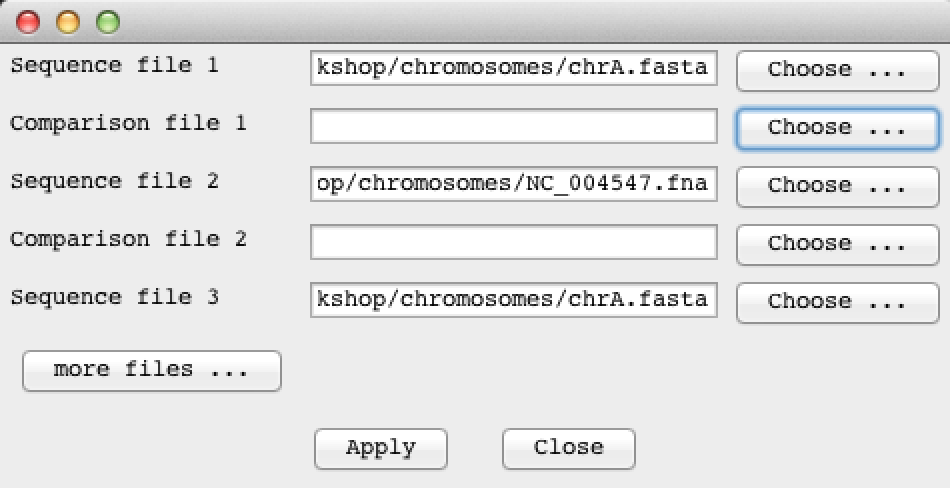
\includegraphics[width=0.9\textwidth]{images/act_wgs4}
      \end{center}
    \end{frame}

    \begin{frame}
      \frametitle{Viewing alignments in ACT}
      Add BLAST/megaBLAST results
      \begin{center}
        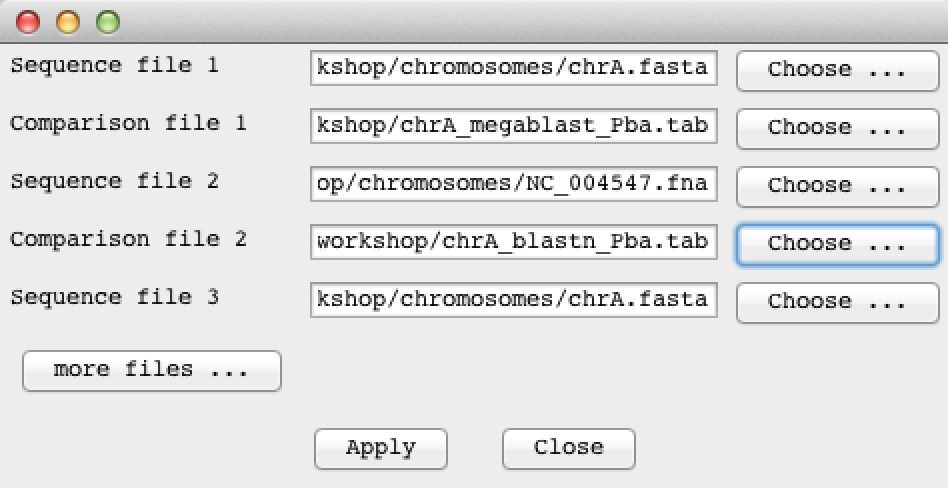
\includegraphics[width=0.9\textwidth]{images/act_wgs5}
      \end{center}
    \end{frame}

    \begin{frame}
      \frametitle{Viewing alignments in ACT}
      After zooming out a bit:
      \begin{center}
        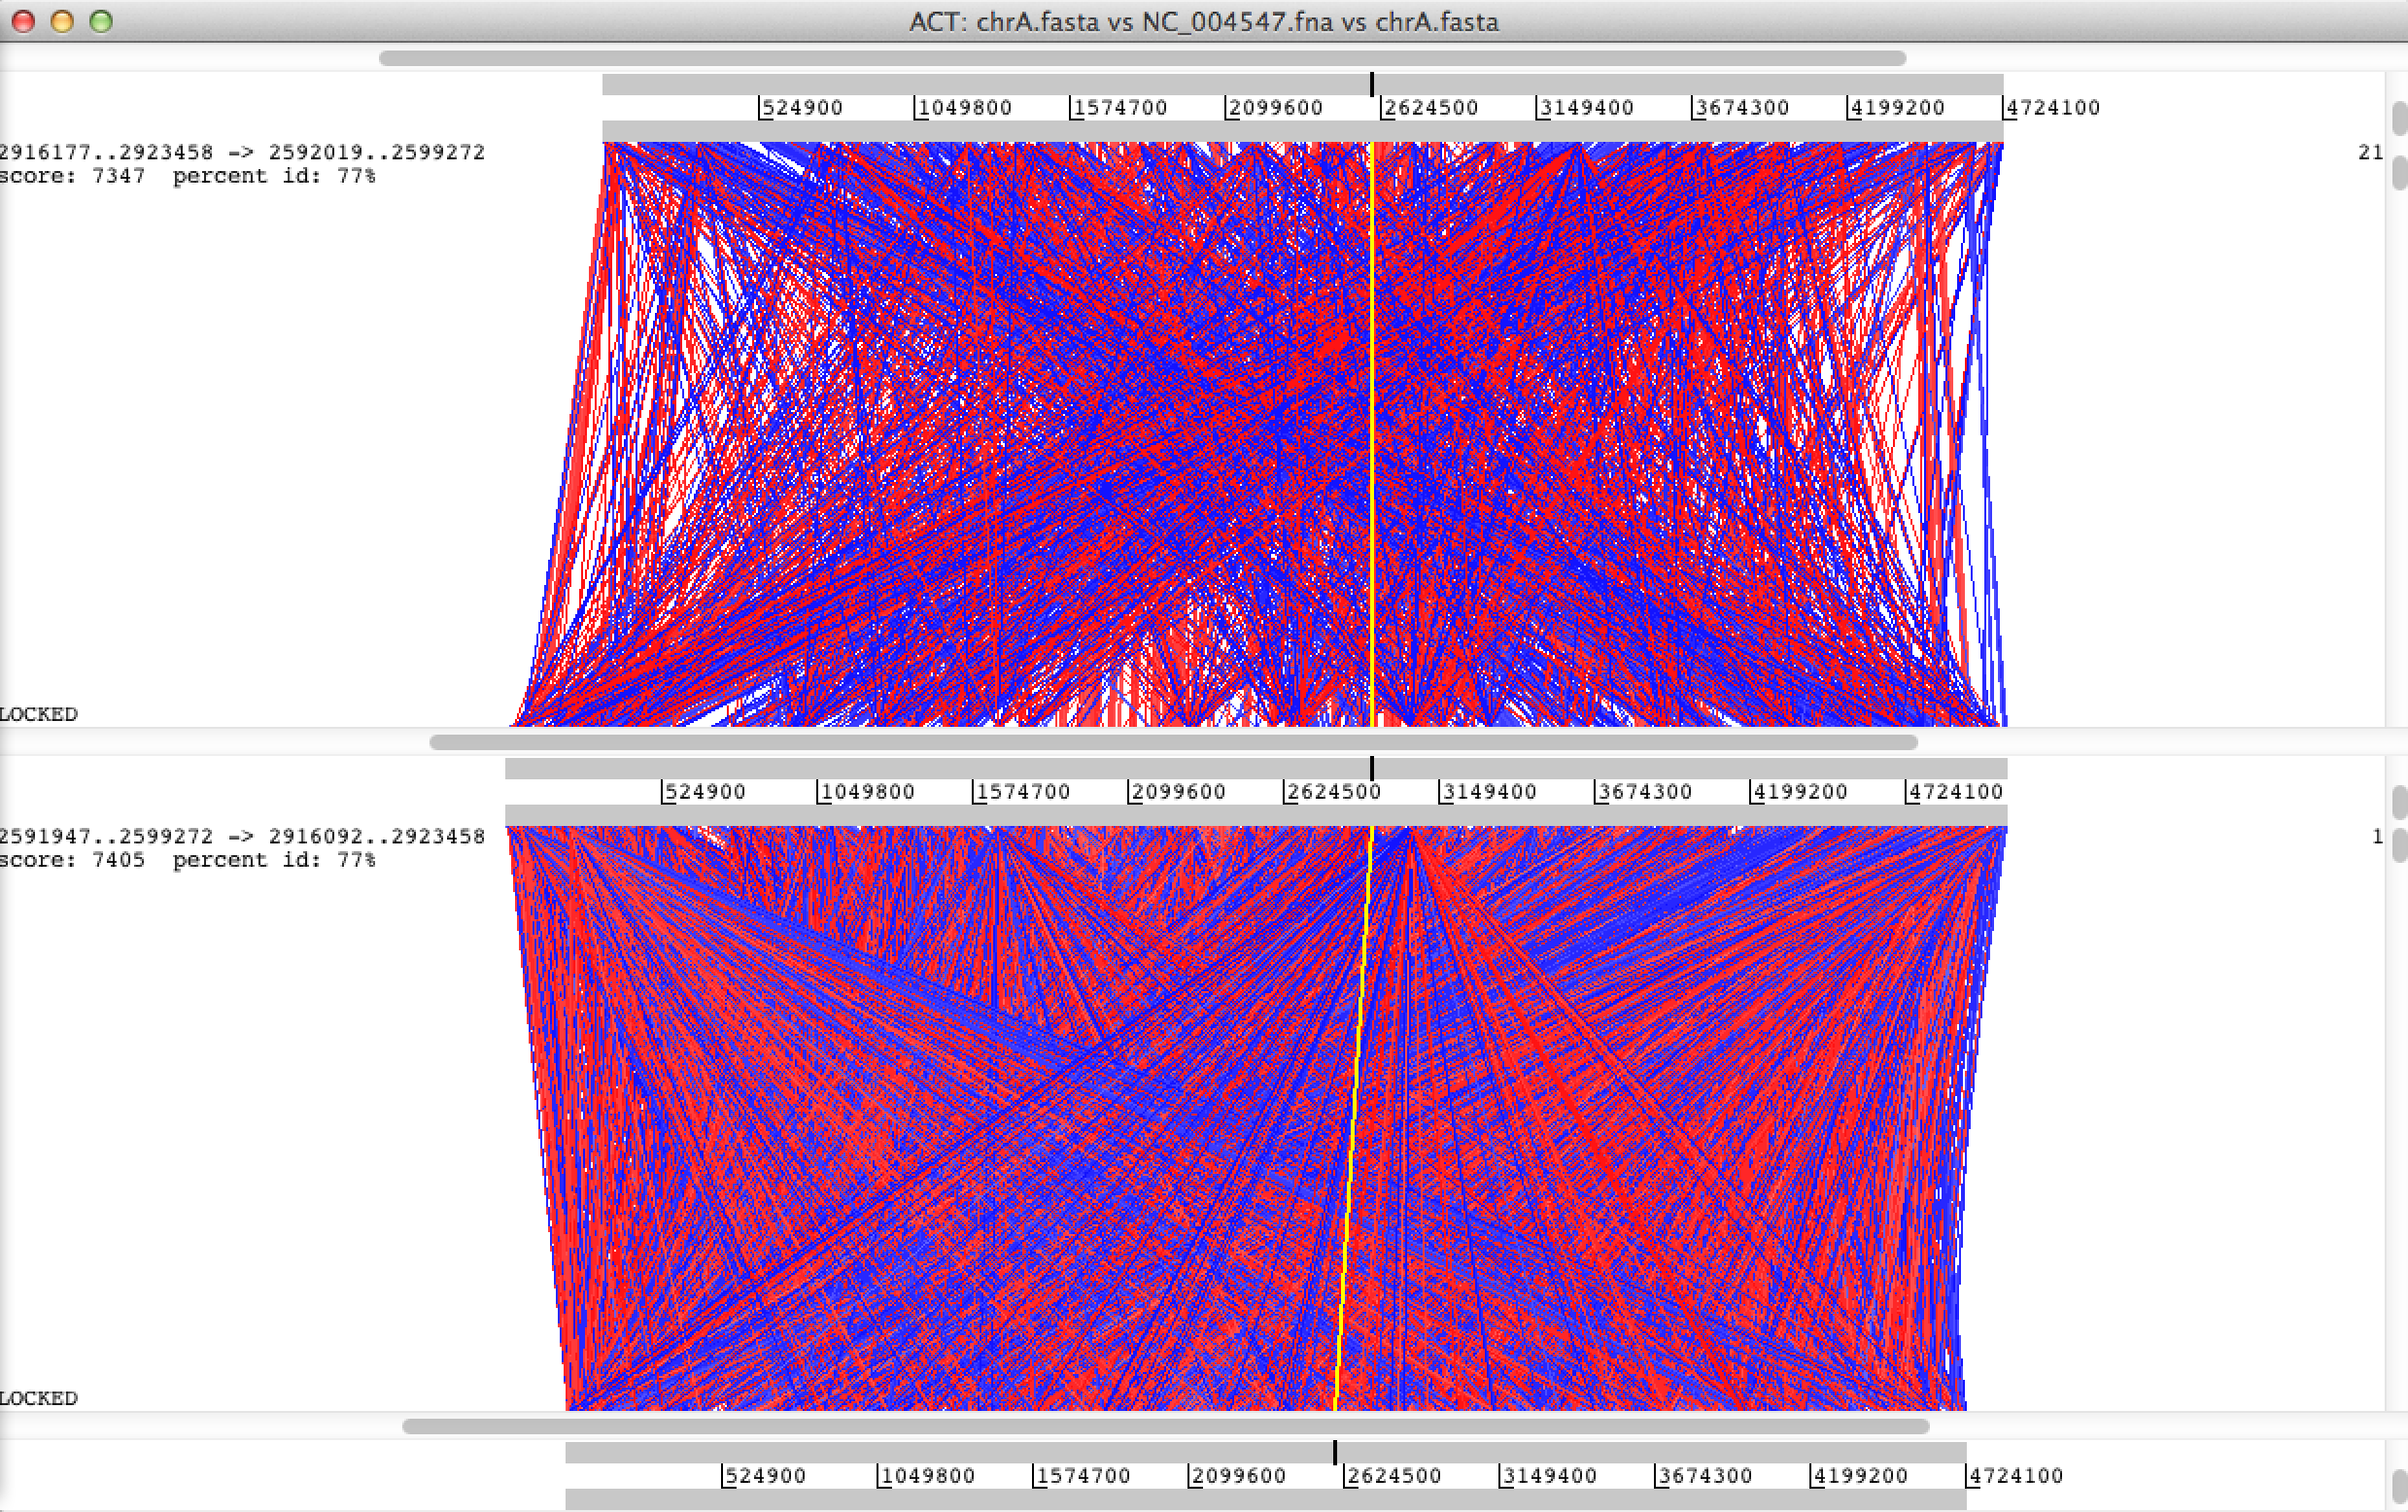
\includegraphics[width=0.8\textwidth]{images/act_wgs6}
      \end{center}
    \end{frame}

    \begin{frame}
      \frametitle{Viewing alignments in ACT}
      Use filter sliders to remove weaker matches
      \begin{center}
        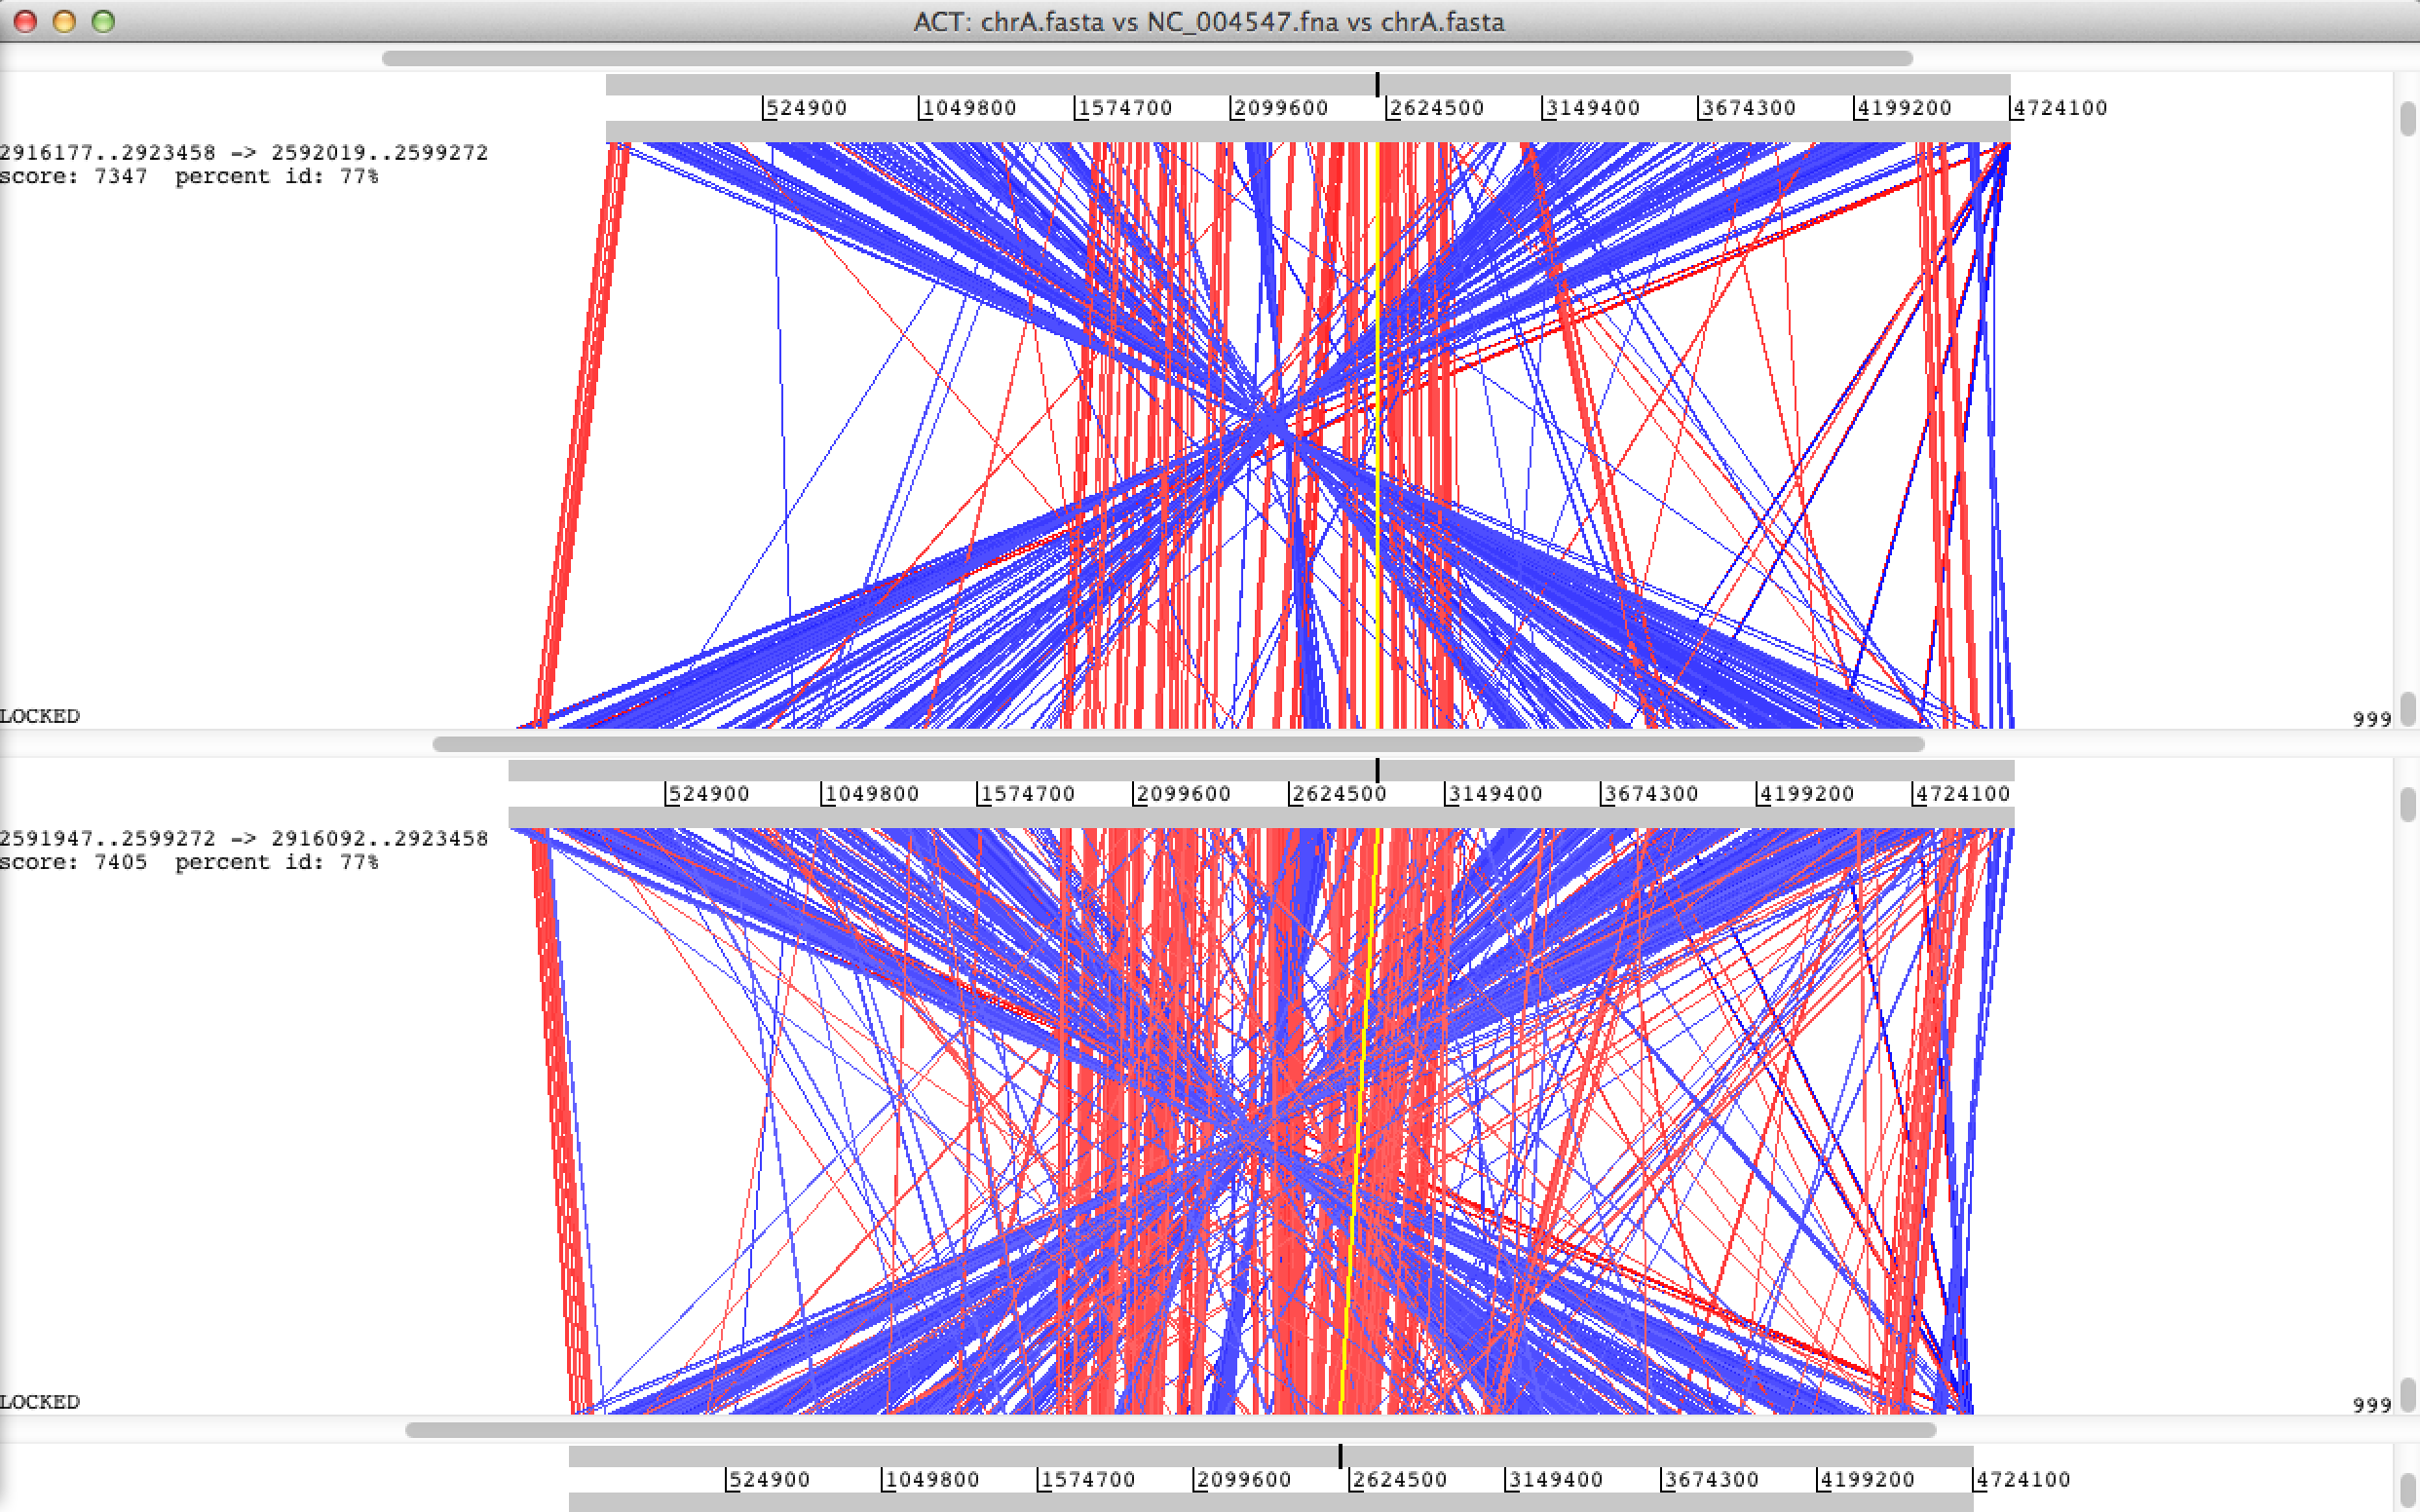
\includegraphics[width=0.8\textwidth]{images/act_wgs7}
      \end{center}
    \end{frame}

\subsection{MUMmer comparisons}

  \begin{frame}
    \frametitle{MUMmer}
    \begin{itemize}
      \item \texttt{MUMmer} is a suite of alignment programs and scripts
      \begin{itemize}
        \item \texttt{mummer}, \texttt{promer}, \texttt{nucmer}, etc.
      \end{itemize}
      \item Very different to BLAST (suffix tree alignment) - very fast
      \item Extremely flexible
      \item Used for genome comparisons, assemblies, scaffolding, repeat detection, etc.
      \item Forms the basis for other aligners/assemblers
    \end{itemize}
\end{frame}

% [fragile] frames must end with \end{frame} directly following a newline, or they break!
  \begin{frame}[fragile]
    \frametitle{Run a MUMmer Comparison}
    Create a new sub-directory for MUMmer output.
\begin{lstlisting}[language=bash]
$ pwd
.../data/workshop/chromosomes
$ mkdir nucmer_out
\end{lstlisting}
    Run \texttt{nucmer} to create \texttt{chrA\_NC\_004547.delta} \\
\begin{lstlisting}[language=bash]
$ nucmer --prefix=nucmer_out/chrA_NC_004547 chrA.fasta NC_004547.fna
\end{lstlisting}
    Then filter this file to generate a coordinate table for visualisation
\begin{lstlisting}[language=bash]
$ delta-filter -q nucmer_out/chrA_NC_004547.delta > nucmer_out/chrA_NC_004547.filter
$ show-coords -rcl nucmer_out/chrA_NC_004547.filter > nucmer_out/chrA_NC_004547_filtered.coords
\end{lstlisting}
\end{frame}

% [fragile] frames must end with \end{frame} directly following a newline, or they break!
  \begin{frame}[fragile]
    \frametitle{Run a MUMmer Comparison}
    MUMmer output is very different from BLAST output
\begin{lstlisting}[language=bash]
$ head nucmer_out/chrA_NC_004547_filtered.coords
...
\end{lstlisting}
\end{frame}

% [fragile] frames must end with \end{frame} directly following a newline, or they break!
  \begin{frame}[fragile]
    \frametitle{Run a MUMmer Comparison}
    Use a one-line shell command to convert to \texttt{ACT}-friendly format:
\begin{lstlisting}[language=bash]
$ tail -n +6 nucmer_out/chrA_NC_004547_filtered.coords | awk '{print $7" "$10" "$1" "$2" "$12" "$4" "$5" "$13}' > chrA_mummer_NC_004547.crunch
$ head chrA_mummer_NC_004547.crunch 
2526 82.49 15 2540 4727782 4985117 4982588 5064019
2944 82.29 2676 5619 4727782 4982544 4979600 5064019
85 95.29 11092 11176 4727782 758690 758774 5064019
1356 81.69 17446 18801 4727782 77639 78994 5064019
\end{lstlisting}
\end{frame}

    \begin{frame}
      \frametitle{Viewing alignments in ACT}    
      Select your chromosome, and the megaBLAST/MUMmer output
      \begin{center}
        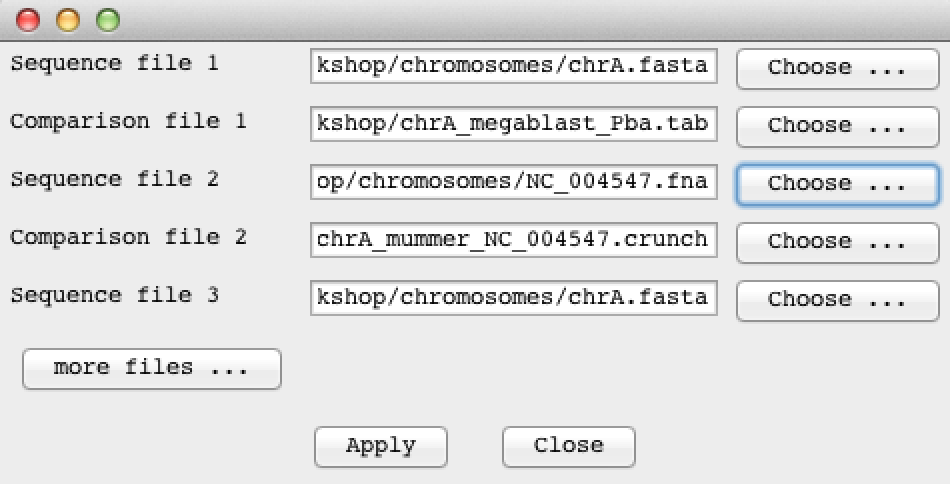
\includegraphics[width=0.9\textwidth]{images/act_wgs8}     
      \end{center}
    \end{frame}

    \begin{frame}
      \frametitle{Viewing alignments in ACT}    
      \begin{center}
        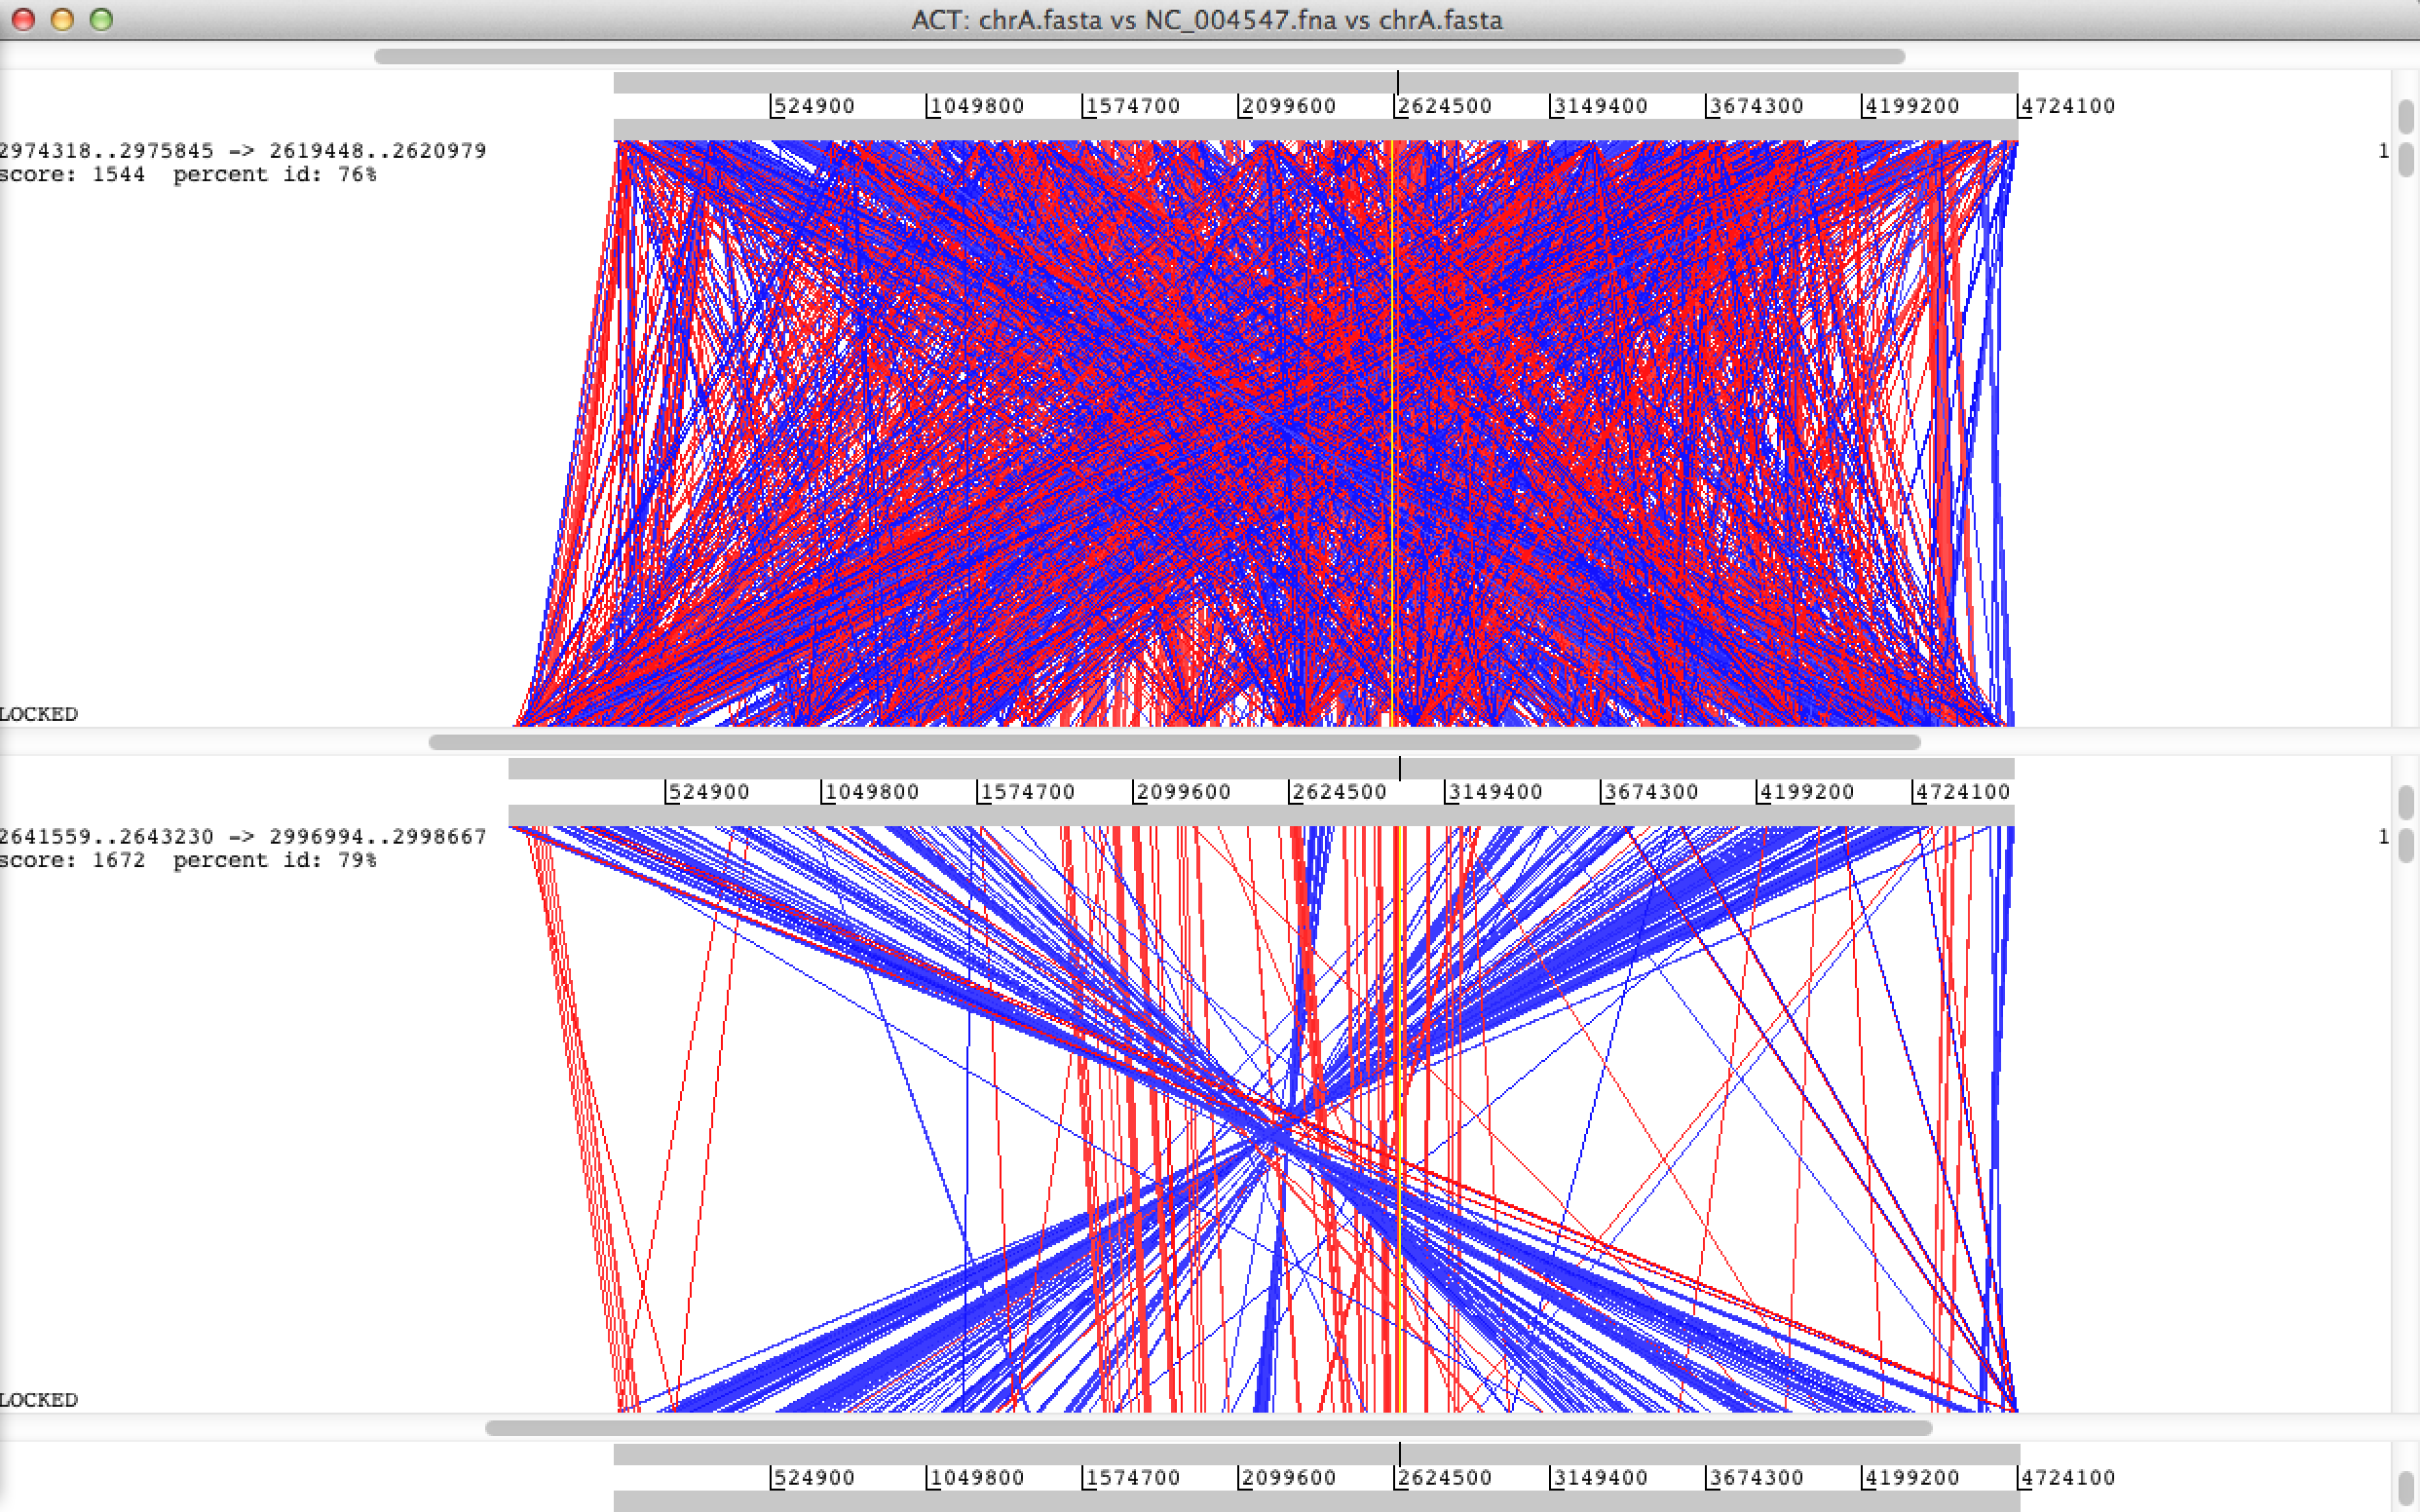
\includegraphics[width=0.8\textwidth]{images/act_wgs9}     
      \end{center}
    \end{frame}

    \begin{frame}
      \frametitle{Viewing alignments in ACT}    
      \begin{center}
        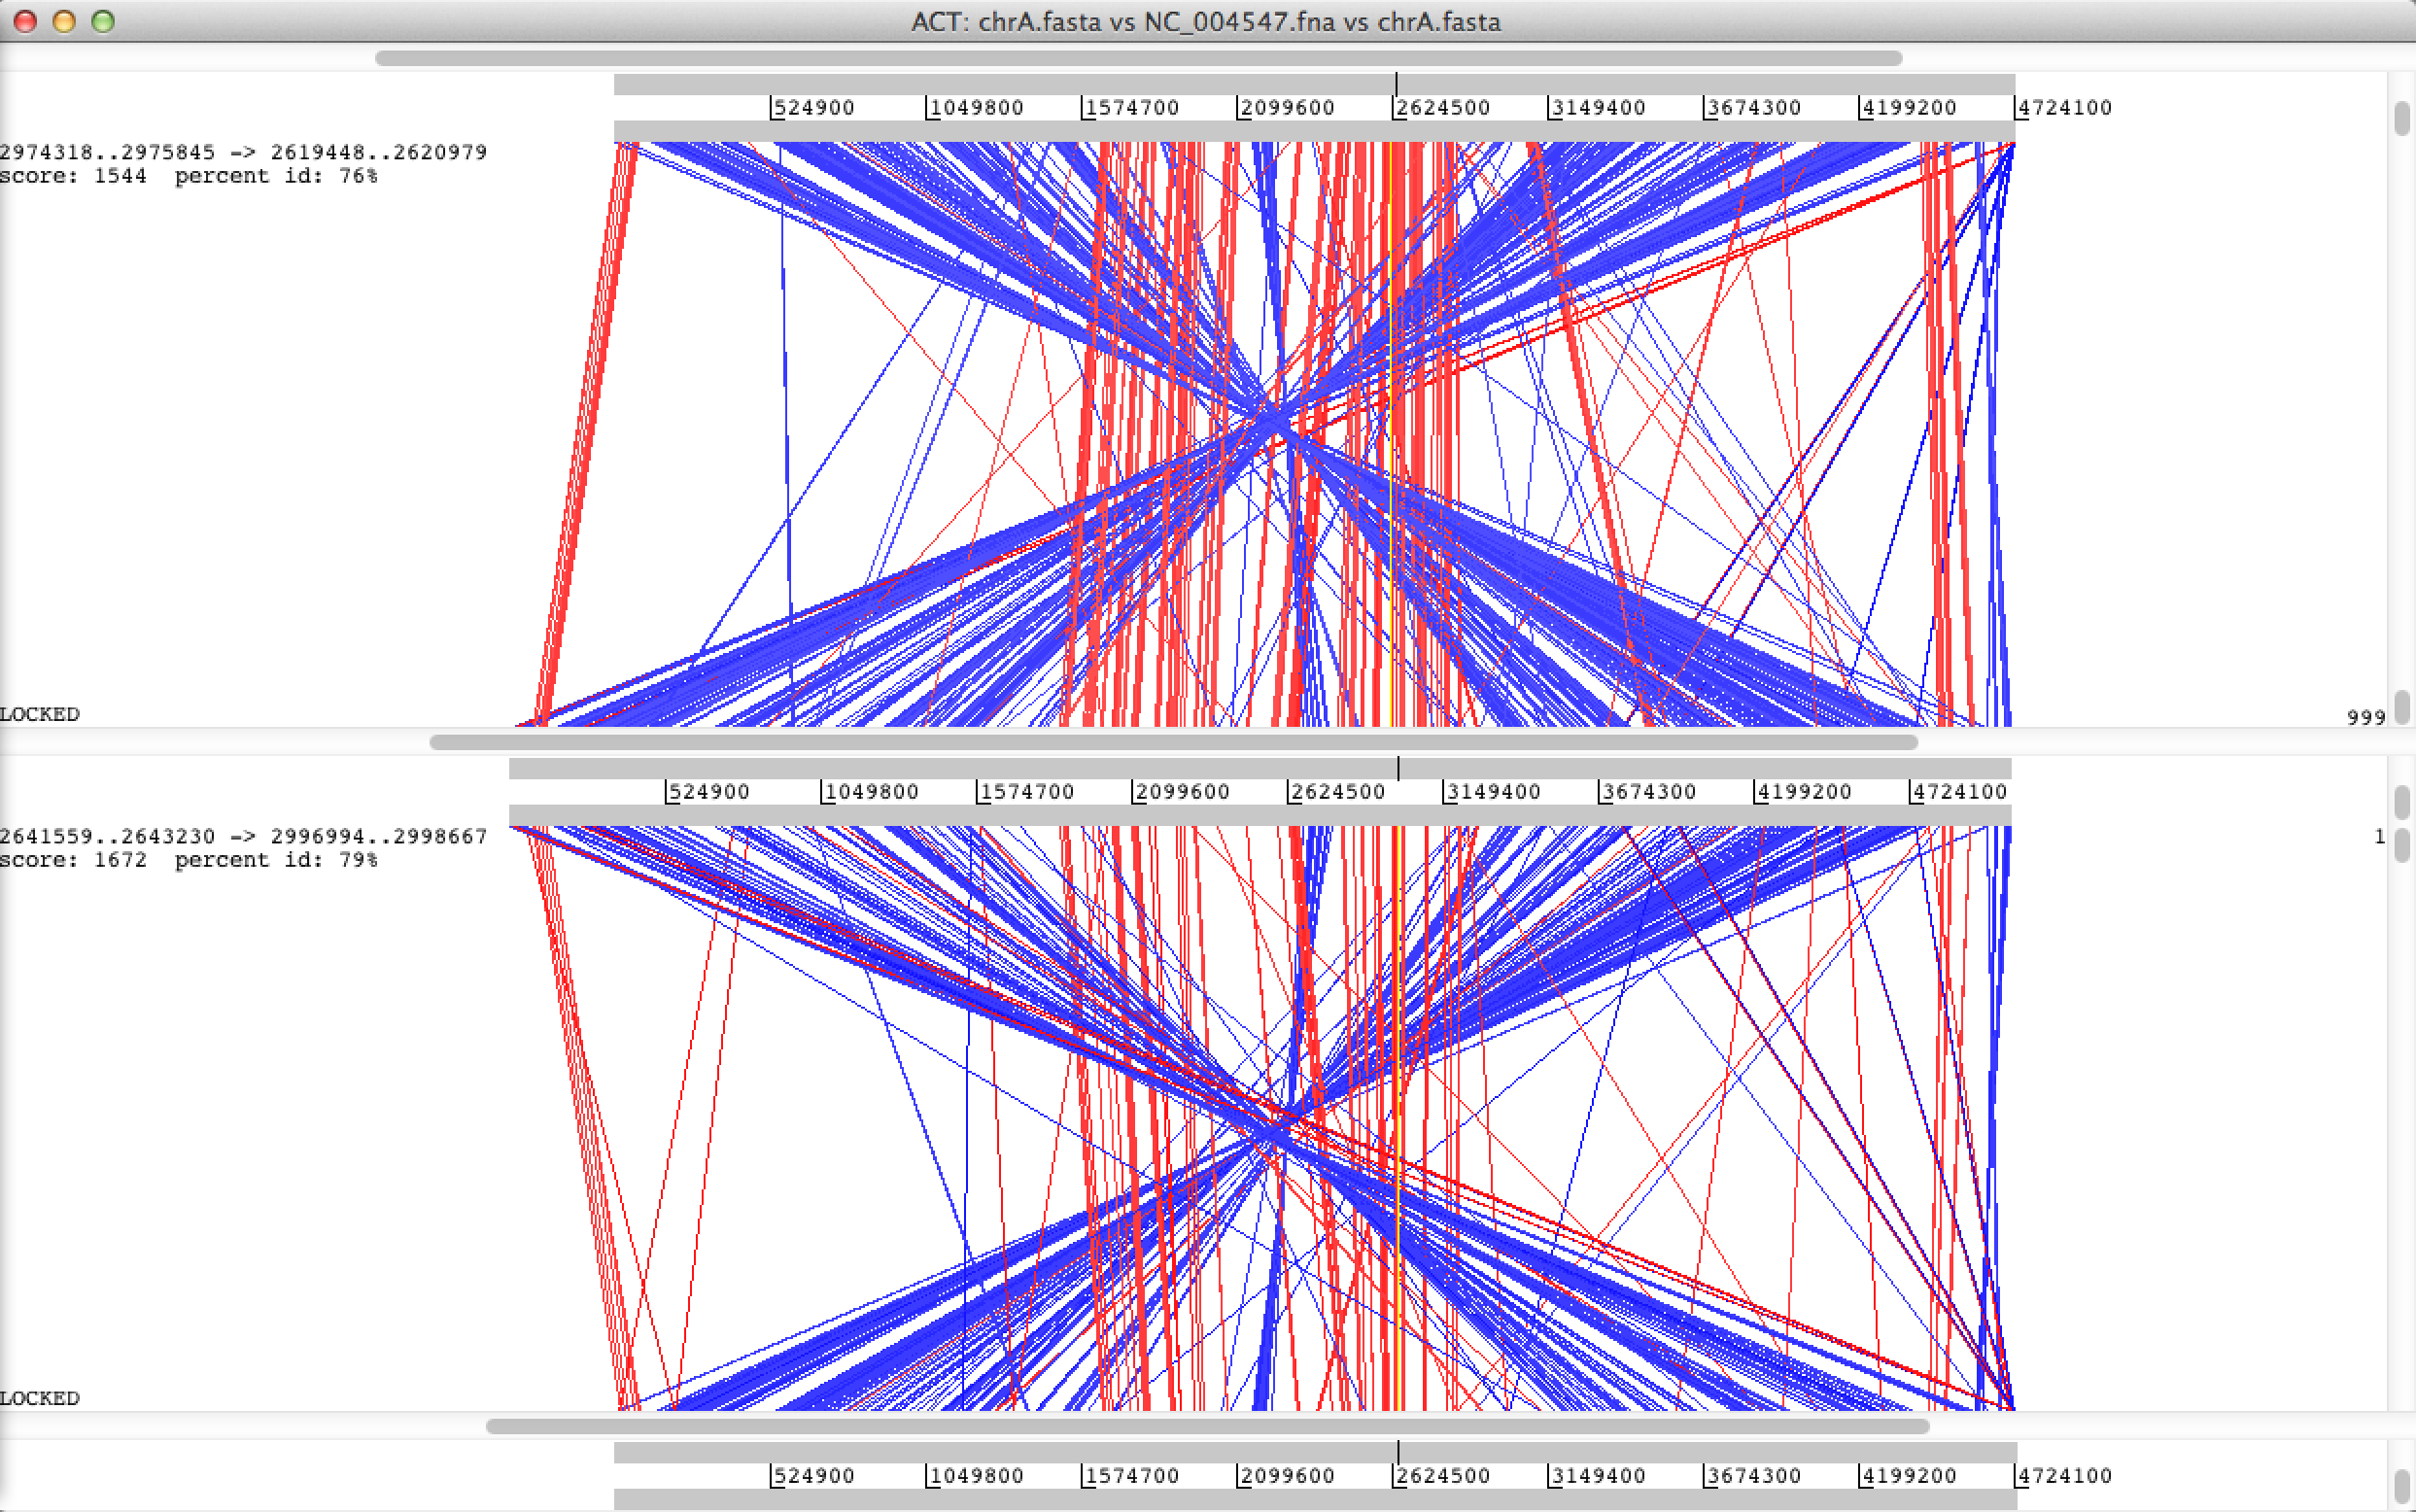
\includegraphics[width=0.8\textwidth]{images/act_wgs10}     
      \end{center}
    \end{frame}

    \begin{frame}
      \frametitle{Genome Alignments}   
      \framesubtitle{Lessons learned}   
      \begin{itemize}
        \item Alignment result depends on algorithm, and parameter choices
        \item Some algorithms/parameter sets more sensitive than others
        \item Appropriate visualisation is essential
      \end{itemize}
    \end{frame}


  % Functional Prediction
  \section{Functional Prediction}
    \begin{frame}
      \frametitle{Methods}   
      Most involve annotation transfer by sequence homology. \\
      Much is dependent on the quality of the alignment, and training set annotation.
      \begin{itemize}
        \item (Blast2GO \url{http://www.blast2go.com/b2ghome})
        \item (KEGG Automatic Annotation Server \url{http://www.genome.jp/kegg/kaas/})
        \item PFam \url{http://www.sanger.ac.uk/resources/databases/pfam.html}
        \item InterProScan \url{http://www.ebi.ac.uk/interpro/interproscan.html}
        \item RAST \url{http://rast.nmpdr.org/}
      \end{itemize}
    \end{frame}

    % PFam
    \subsection{PFam}
    \begin{frame}
      \frametitle{How PFam Works}   
      \begin{itemize}
        \item [PFam-A] Curators identify domains of interest (may or may not have known function)
        \item [PFam-B] Sequence segments (from the ADDA domain sequence database) that don't match PFam-A are automatically grouped into families
        \item A seed alignment is constructed from representative sequences
      \end{itemize}
      \begin{center}
        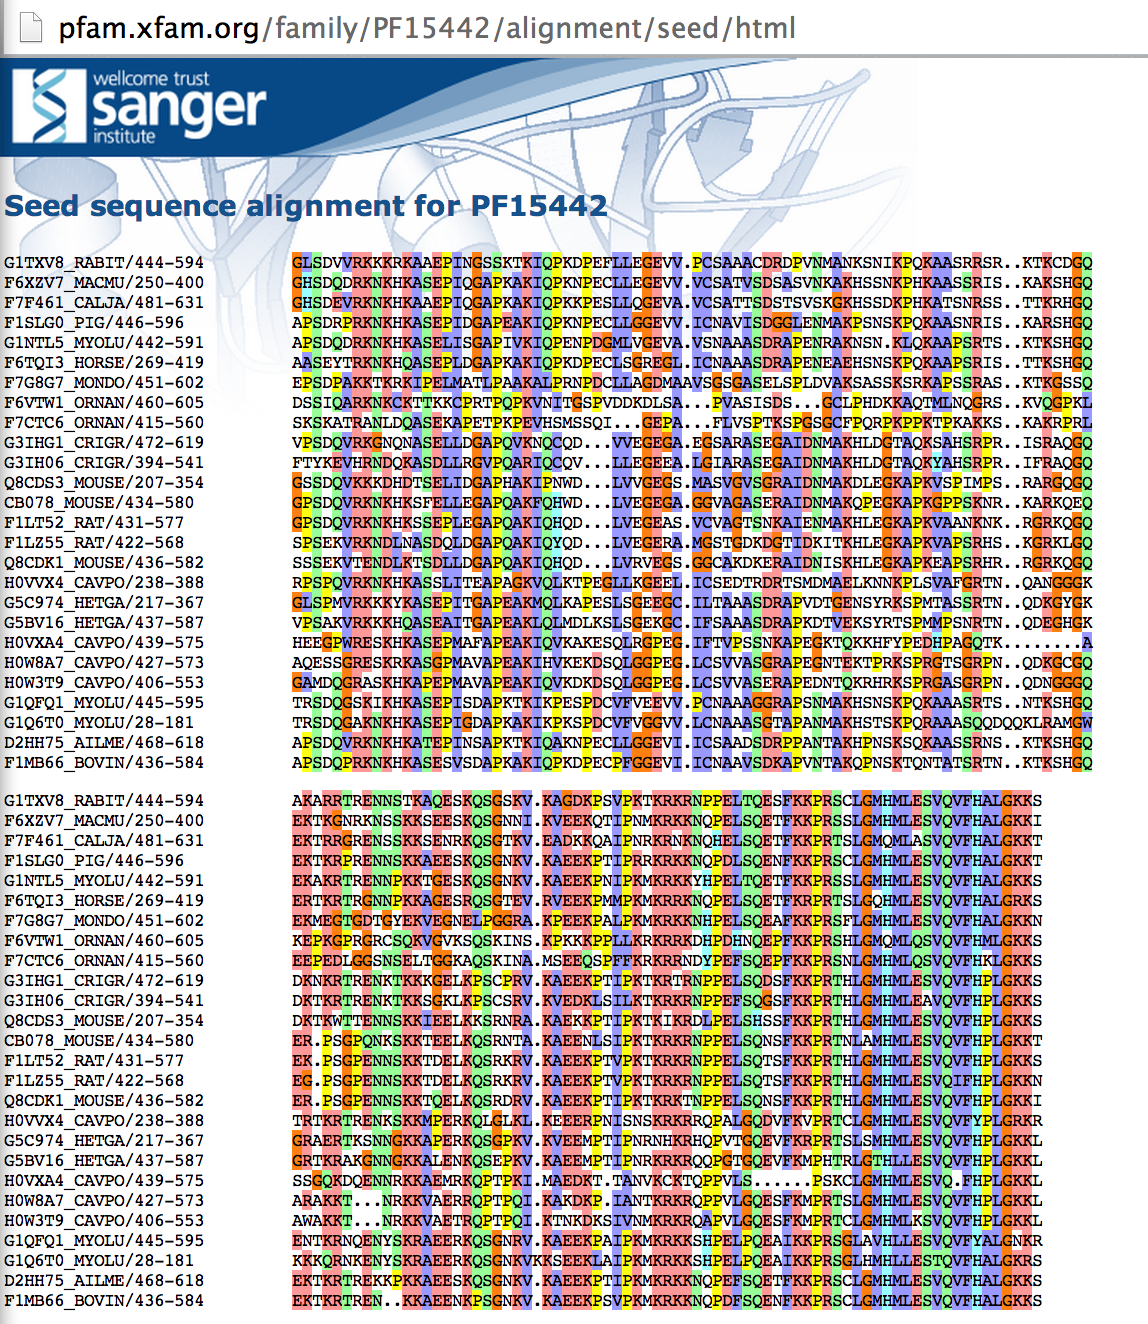
\includegraphics[width=0.3\textwidth]{images/pfam1}     
      \end{center}      
    \end{frame}

    \begin{frame}
      \frametitle{How PFam Works}   
      \begin{itemize}
        \item A profile HMM is built from the seed alignment, using HMMer
        \item Profile HMMs can be represented as sequence logos
      \end{itemize}
      \begin{center}
        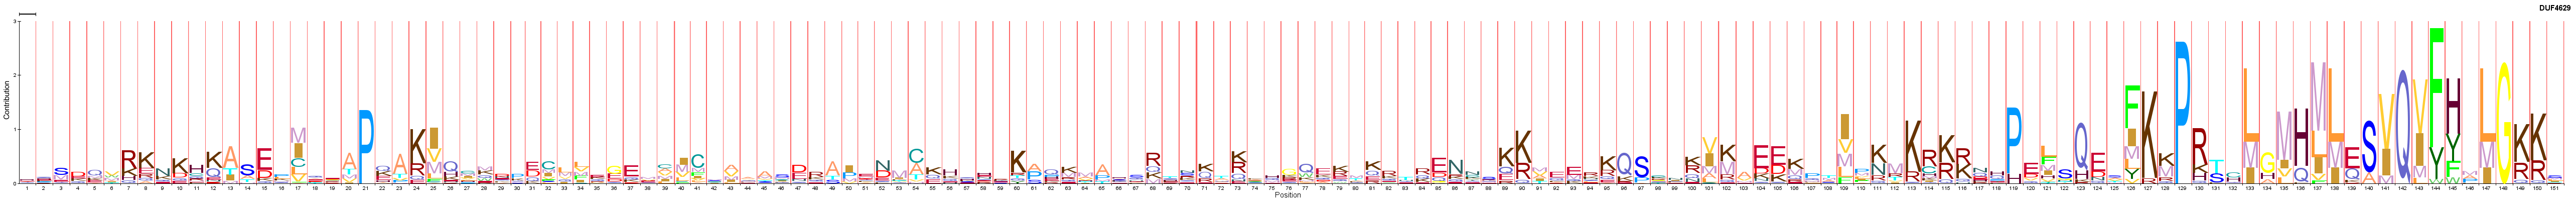
\includegraphics[width=0.9\textwidth]{images/pfam2} 
      \end{center}      
    \end{frame}

    \begin{frame}
      \frametitle{How PFam Works}   
      \begin{itemize}
        \item Profile HMM used to query several sequence databases, to generate full alignment
        \item Curated thresholds are used to determine family membership
      \end{itemize}
      \begin{center}
        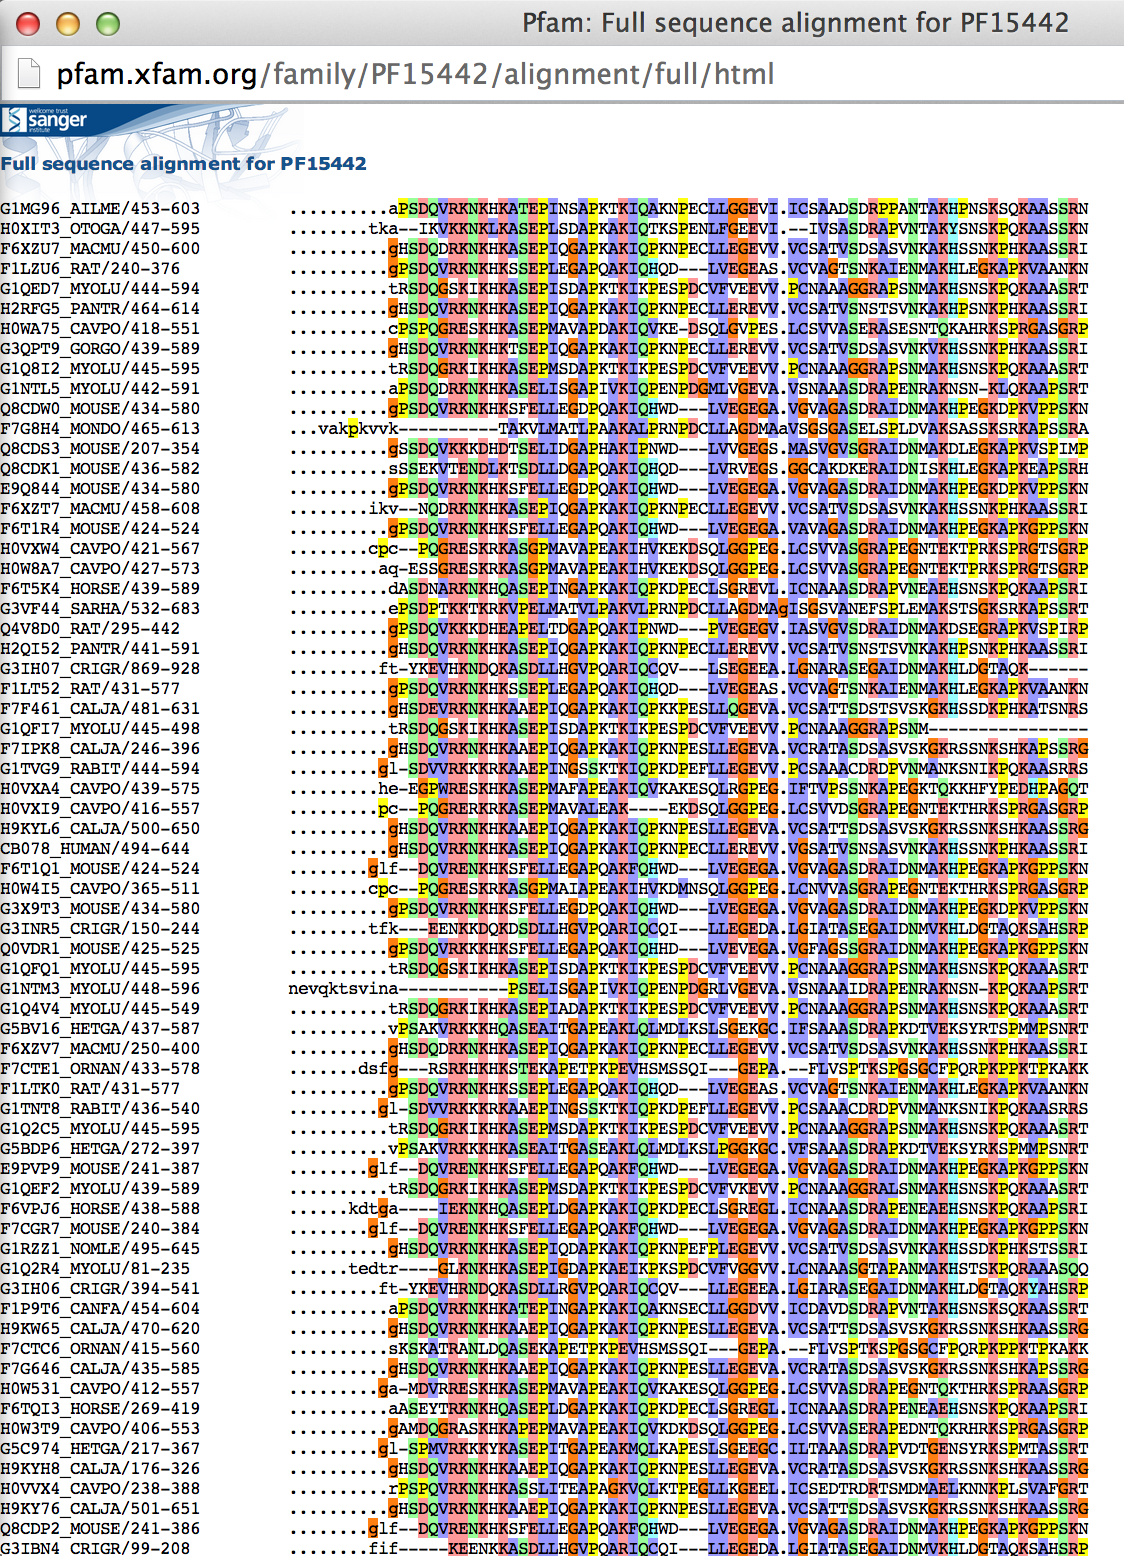
\includegraphics[width=0.3\textwidth]{images/pfam3} 
      \end{center}      
    \end{frame}

    \begin{frame}
      \frametitle{How PFam Works}  
      Bit score is used, not E-value
      \begin{itemize}
        \item [GA] Gathering threshold: Manually-determined for each family, used to build full alignment. Set to exclude false positives 
        \item [TC] Trusted cutoff: Lowest sequence score and domain score of match in the full alignment
        \item [NC] Noise cutoff: Highest sequence score and domain score of match not in full alignment
      \end{itemize}
      \begin{center}
        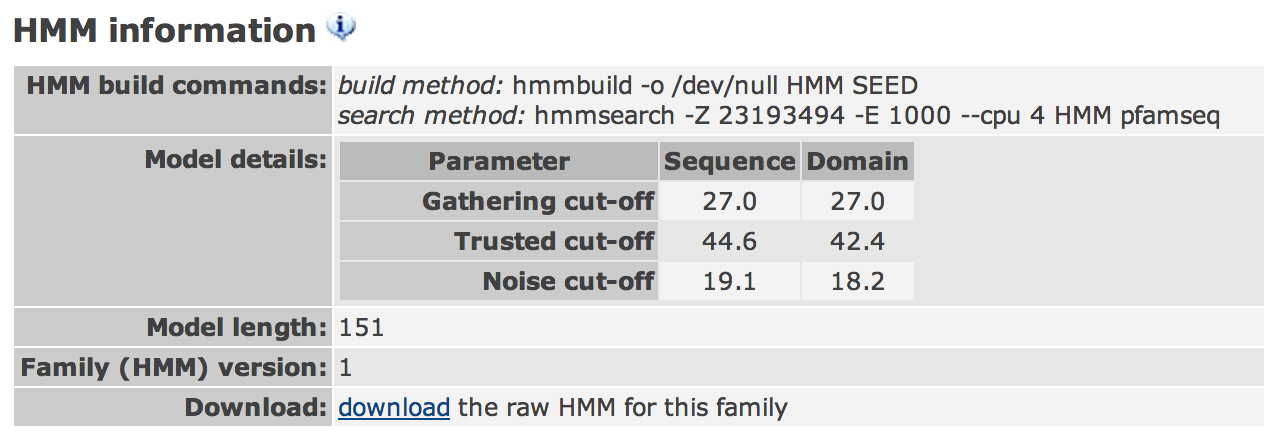
\includegraphics[width=0.5\textwidth]{images/pfam4} 
      \end{center}      
    \end{frame}

    \begin{frame}
      \frametitle{PFam example}  
      Choose a sequence from your annotated draft genome, in Artemis \\
      \begin{center}
        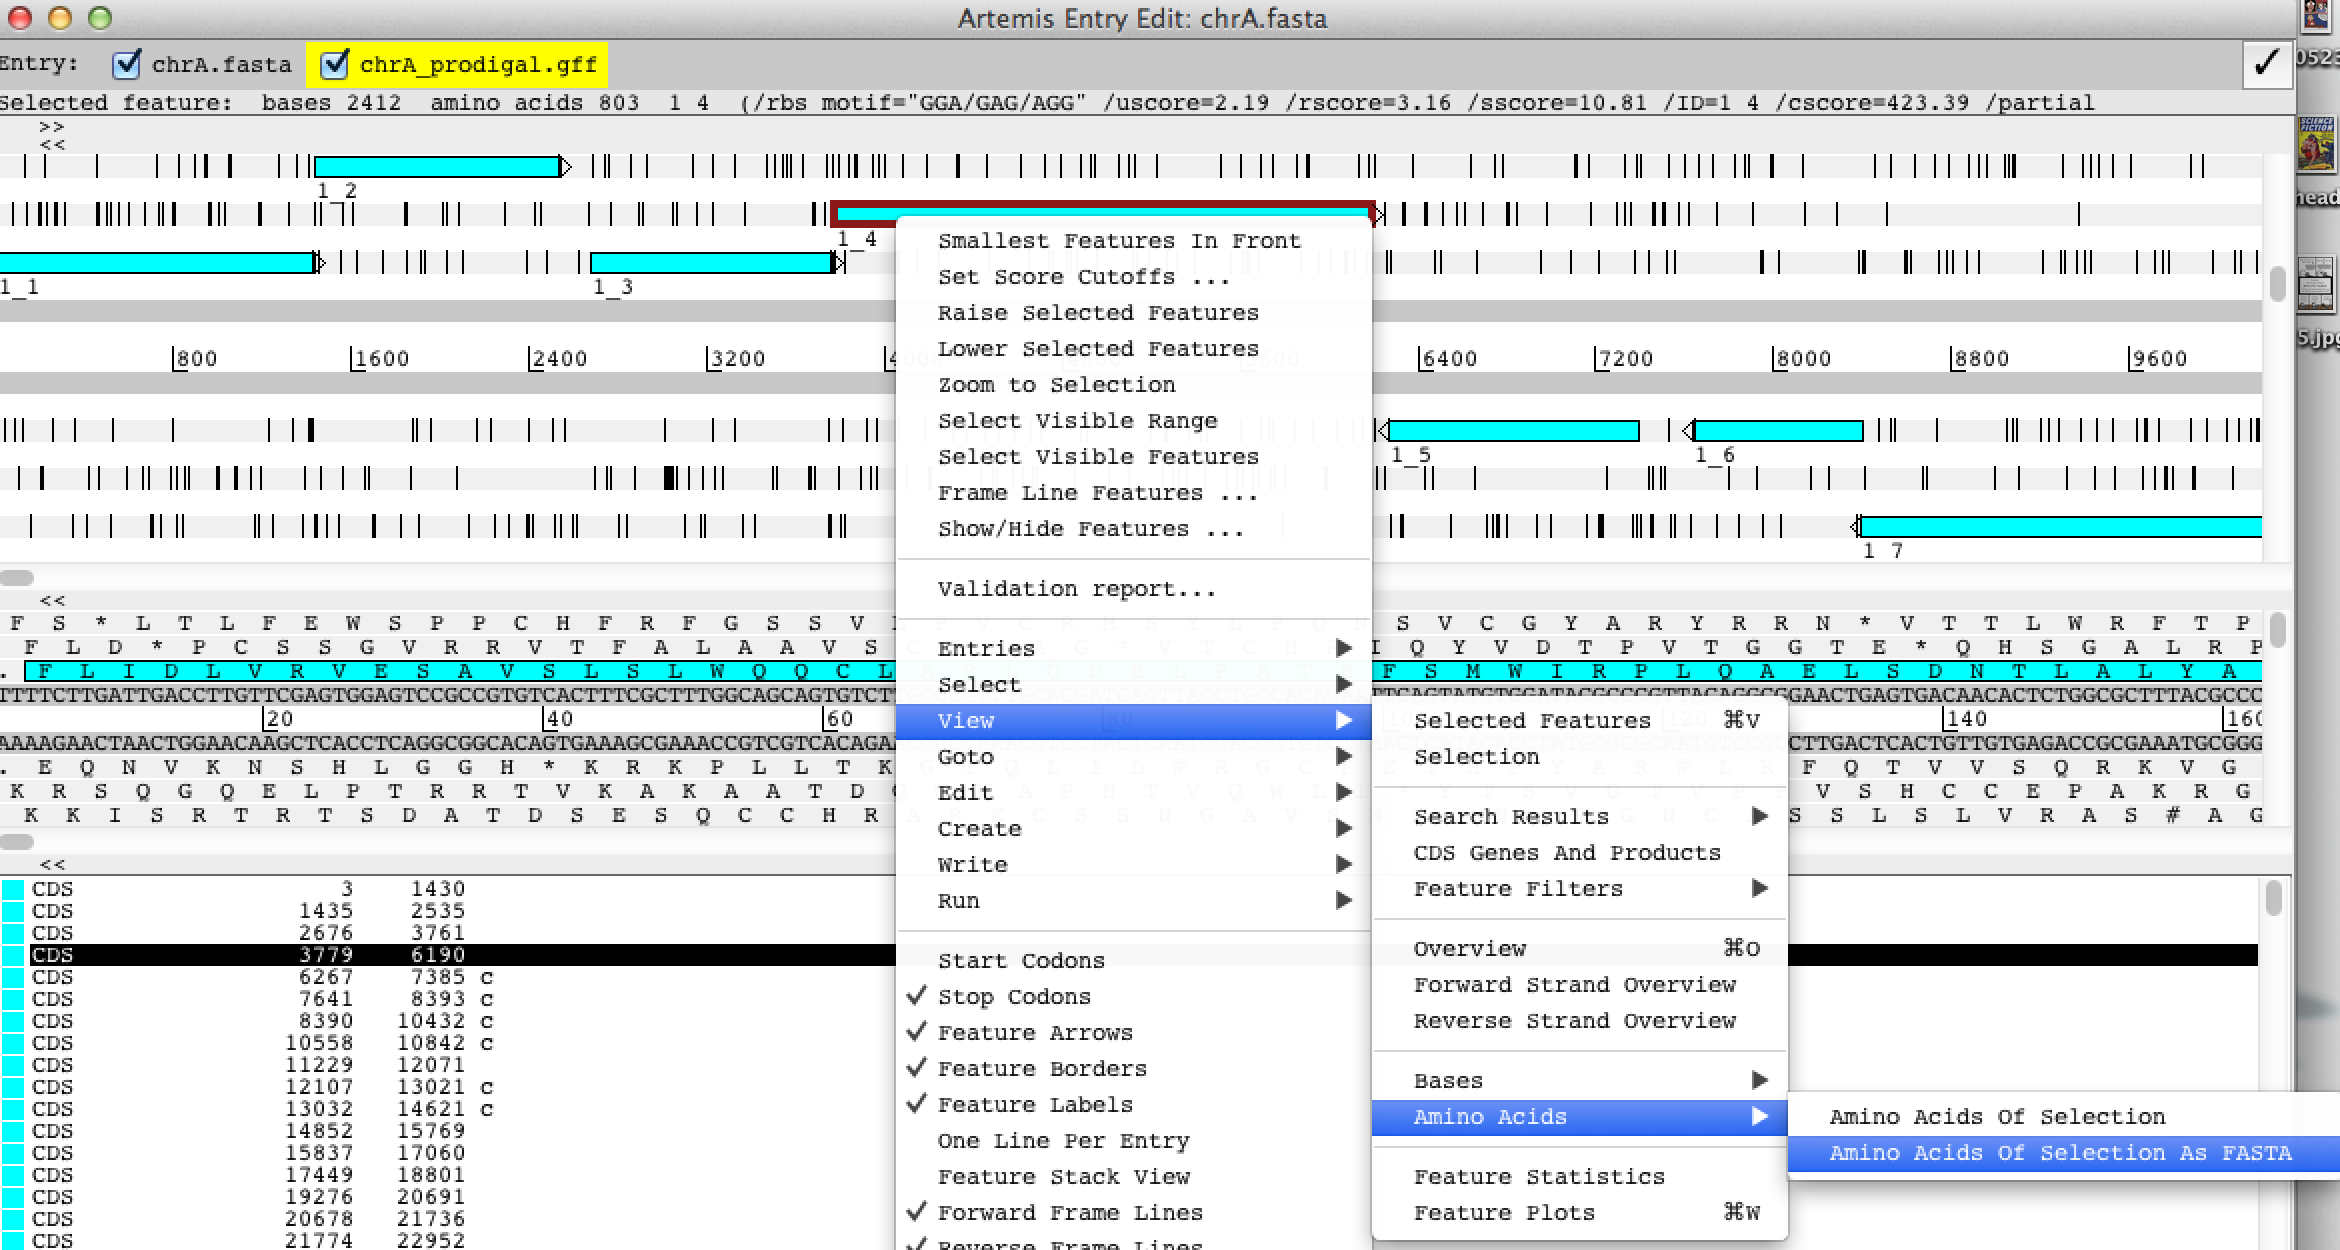
\includegraphics[width=0.9\textwidth]{images/pfam5} 
      \end{center}      
    \end{frame}

    \begin{frame}
      \frametitle{PFam example}  
      Copy the sequence to clipboard
      \begin{center}
        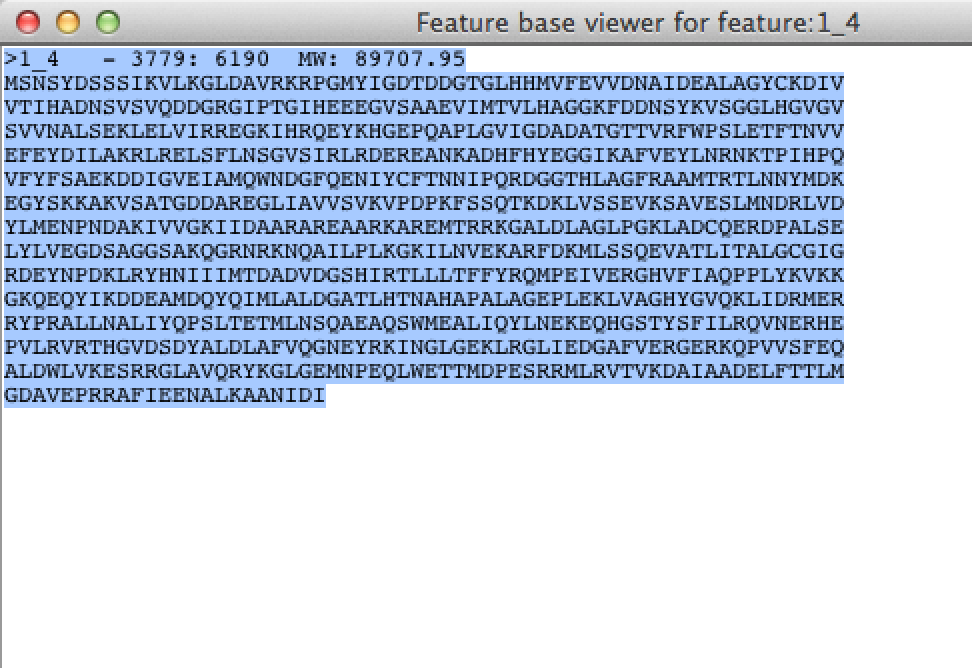
\includegraphics[width=0.5\textwidth]{images/pfam6} 
      \end{center}      
    \end{frame}

    \begin{frame}
      \frametitle{PFam example}  
      Open \url{http://pfam.xfam.org/} in your browser \\
      Click on "SEQUENCE SEARCH"
      \begin{center}
        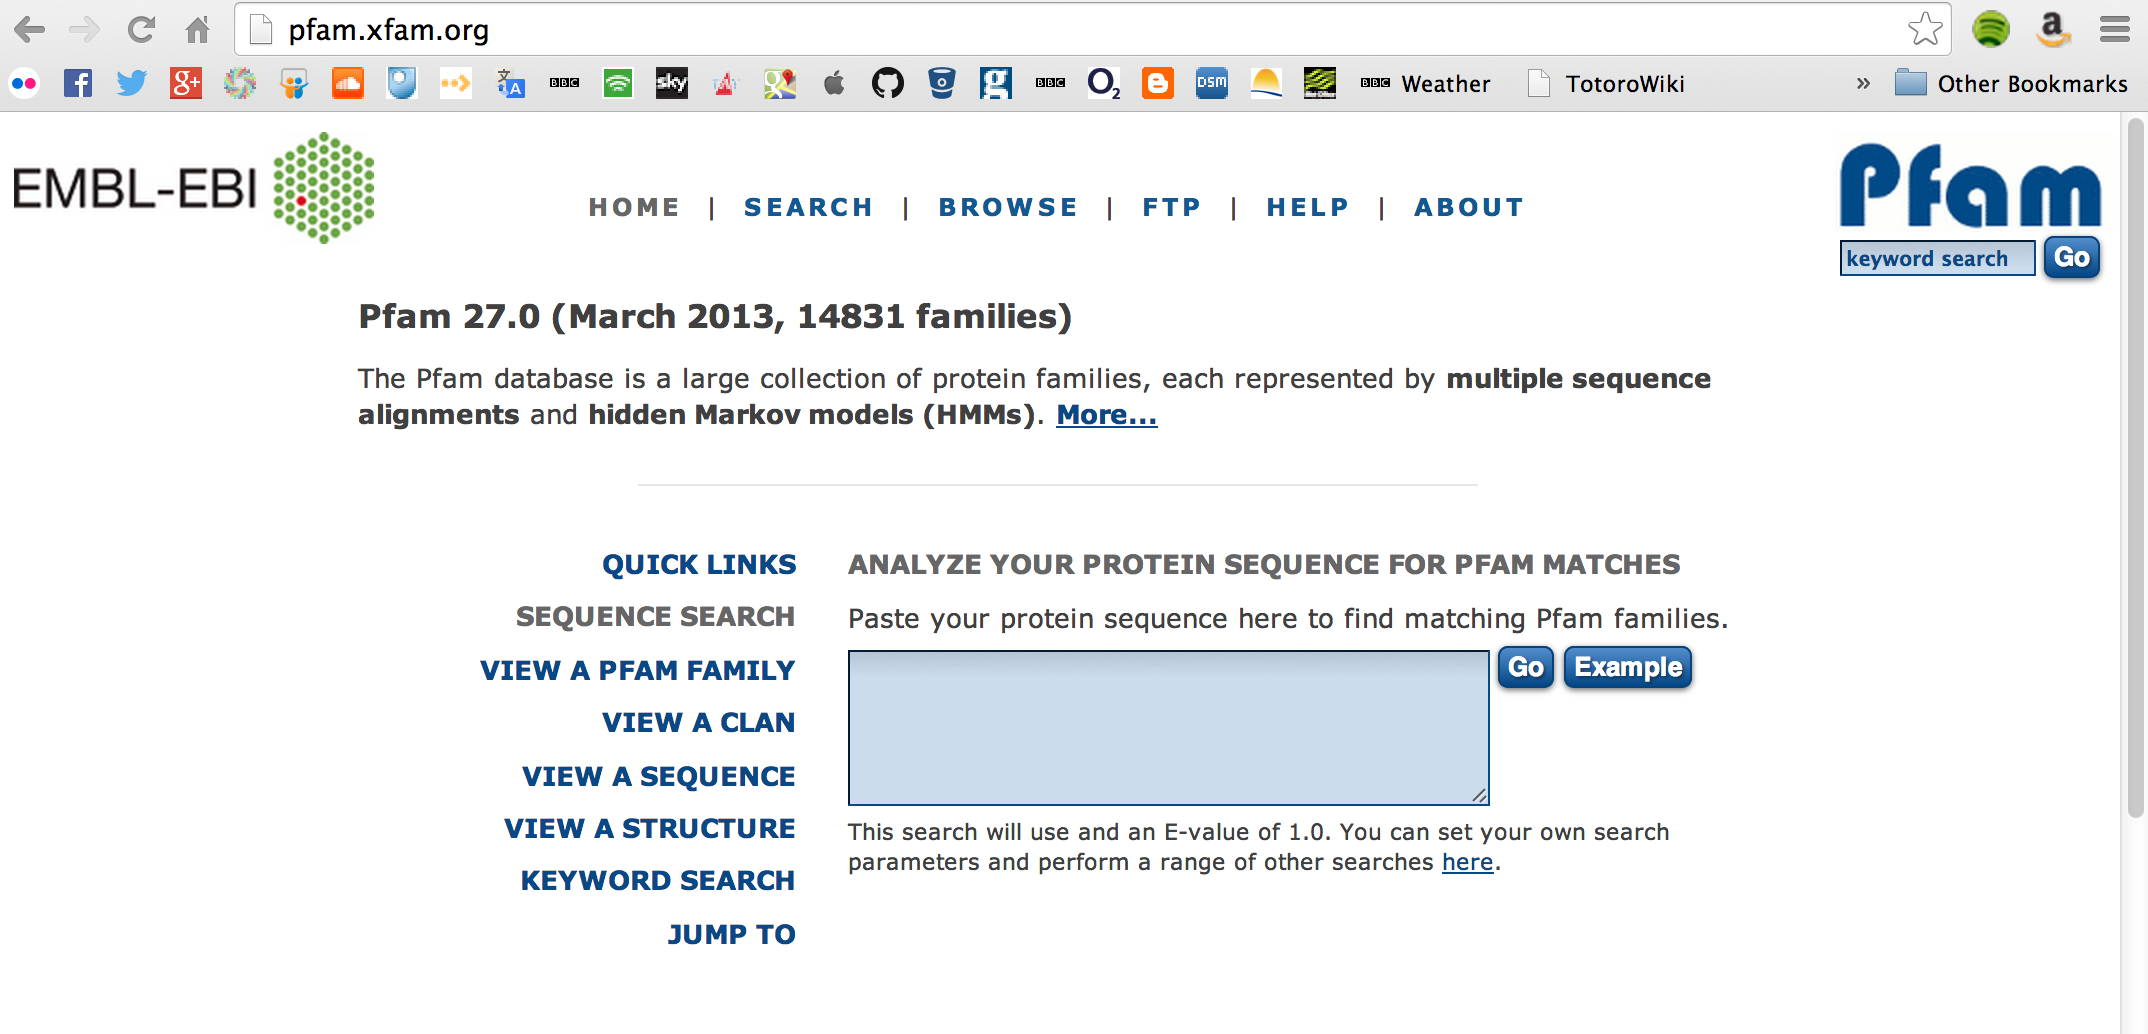
\includegraphics[width=0.9\textwidth]{images/pfam7} 
      \end{center}      
    \end{frame}

    \begin{frame}
      \frametitle{PFam example}  
      Paste your sequence and click "Go"
      \begin{center}
        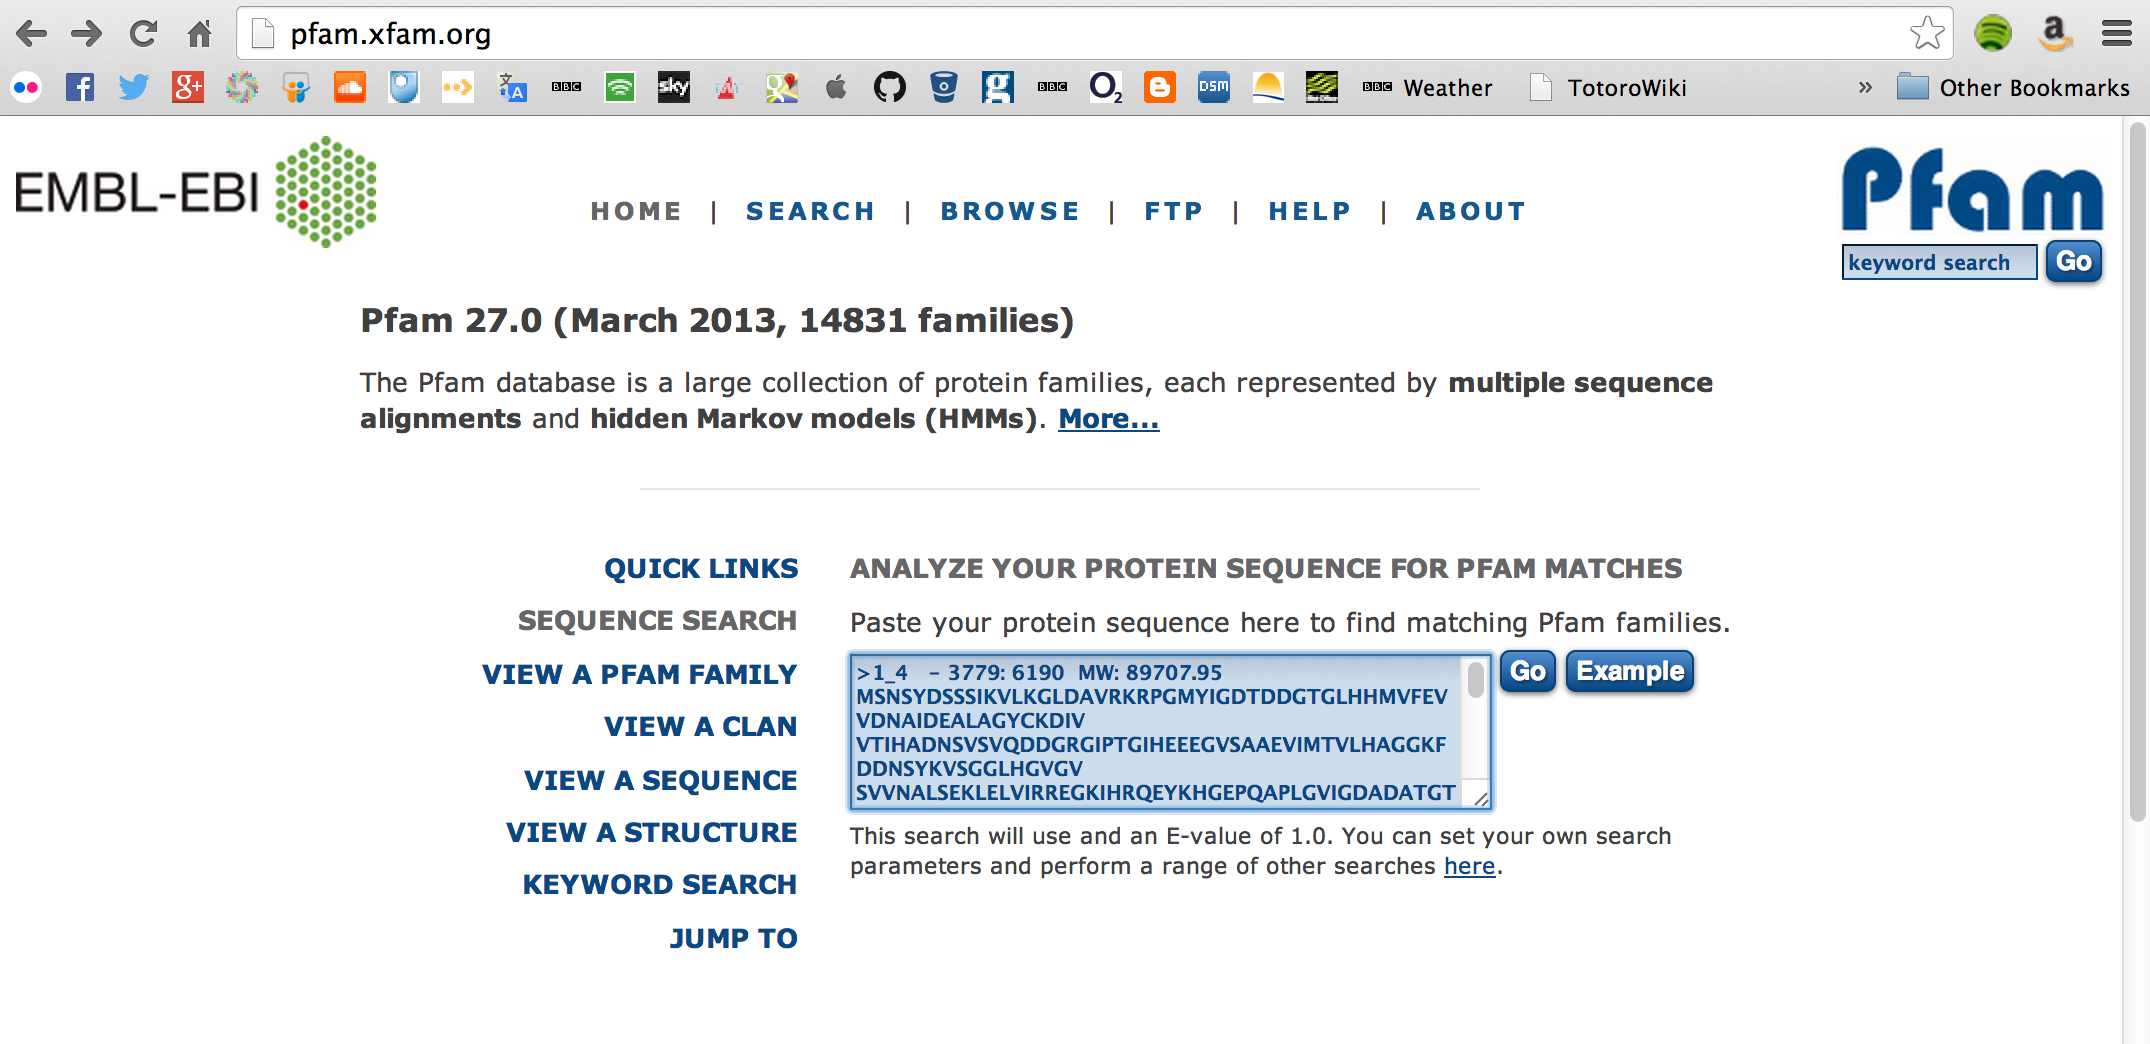
\includegraphics[width=0.9\textwidth]{images/pfam8} 
      \end{center}      
    \end{frame}

    \begin{frame}
      \frametitle{PFam example}  
      Domain matches are returned \\
      (but maybe not for your choice of CDS$\ldots$)
      \begin{center}
        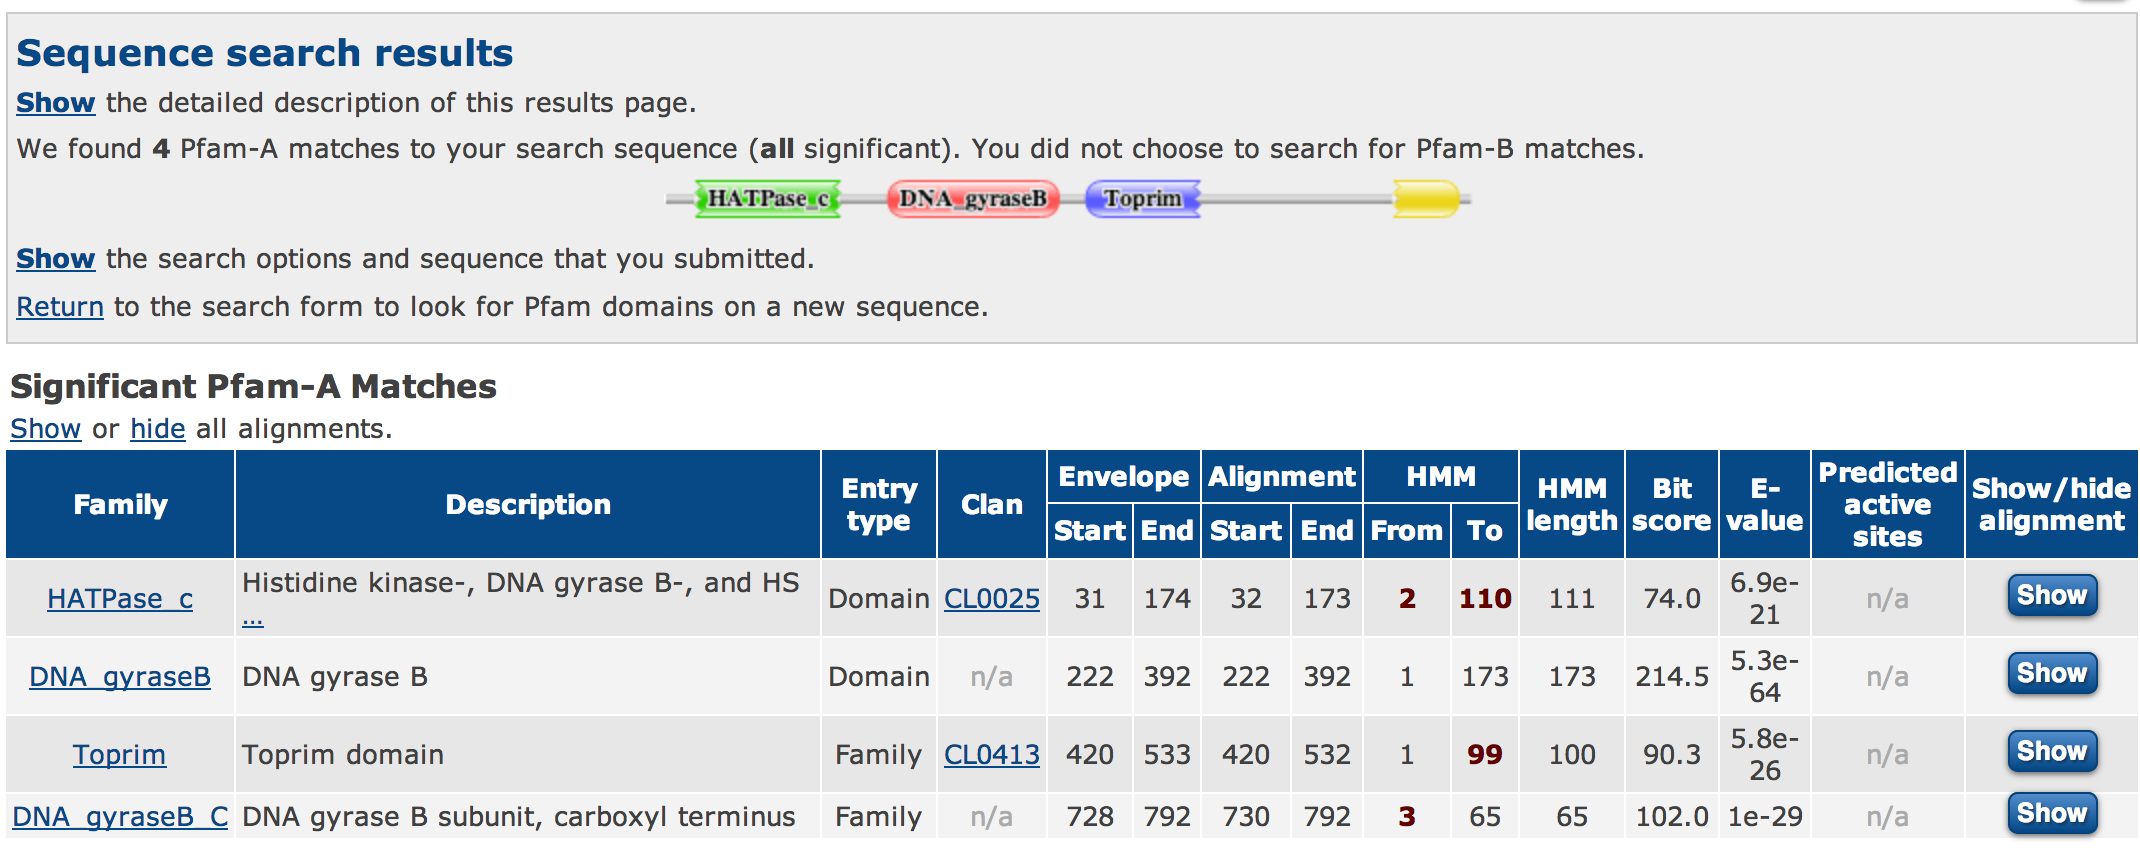
\includegraphics[width=0.9\textwidth]{images/pfam9} 
      \end{center}      
    \end{frame}

    \begin{frame}
      \frametitle{PFam example}  
      Compare match bit scores to GA, TC, NC thresholds for each domain
      \begin{center}
        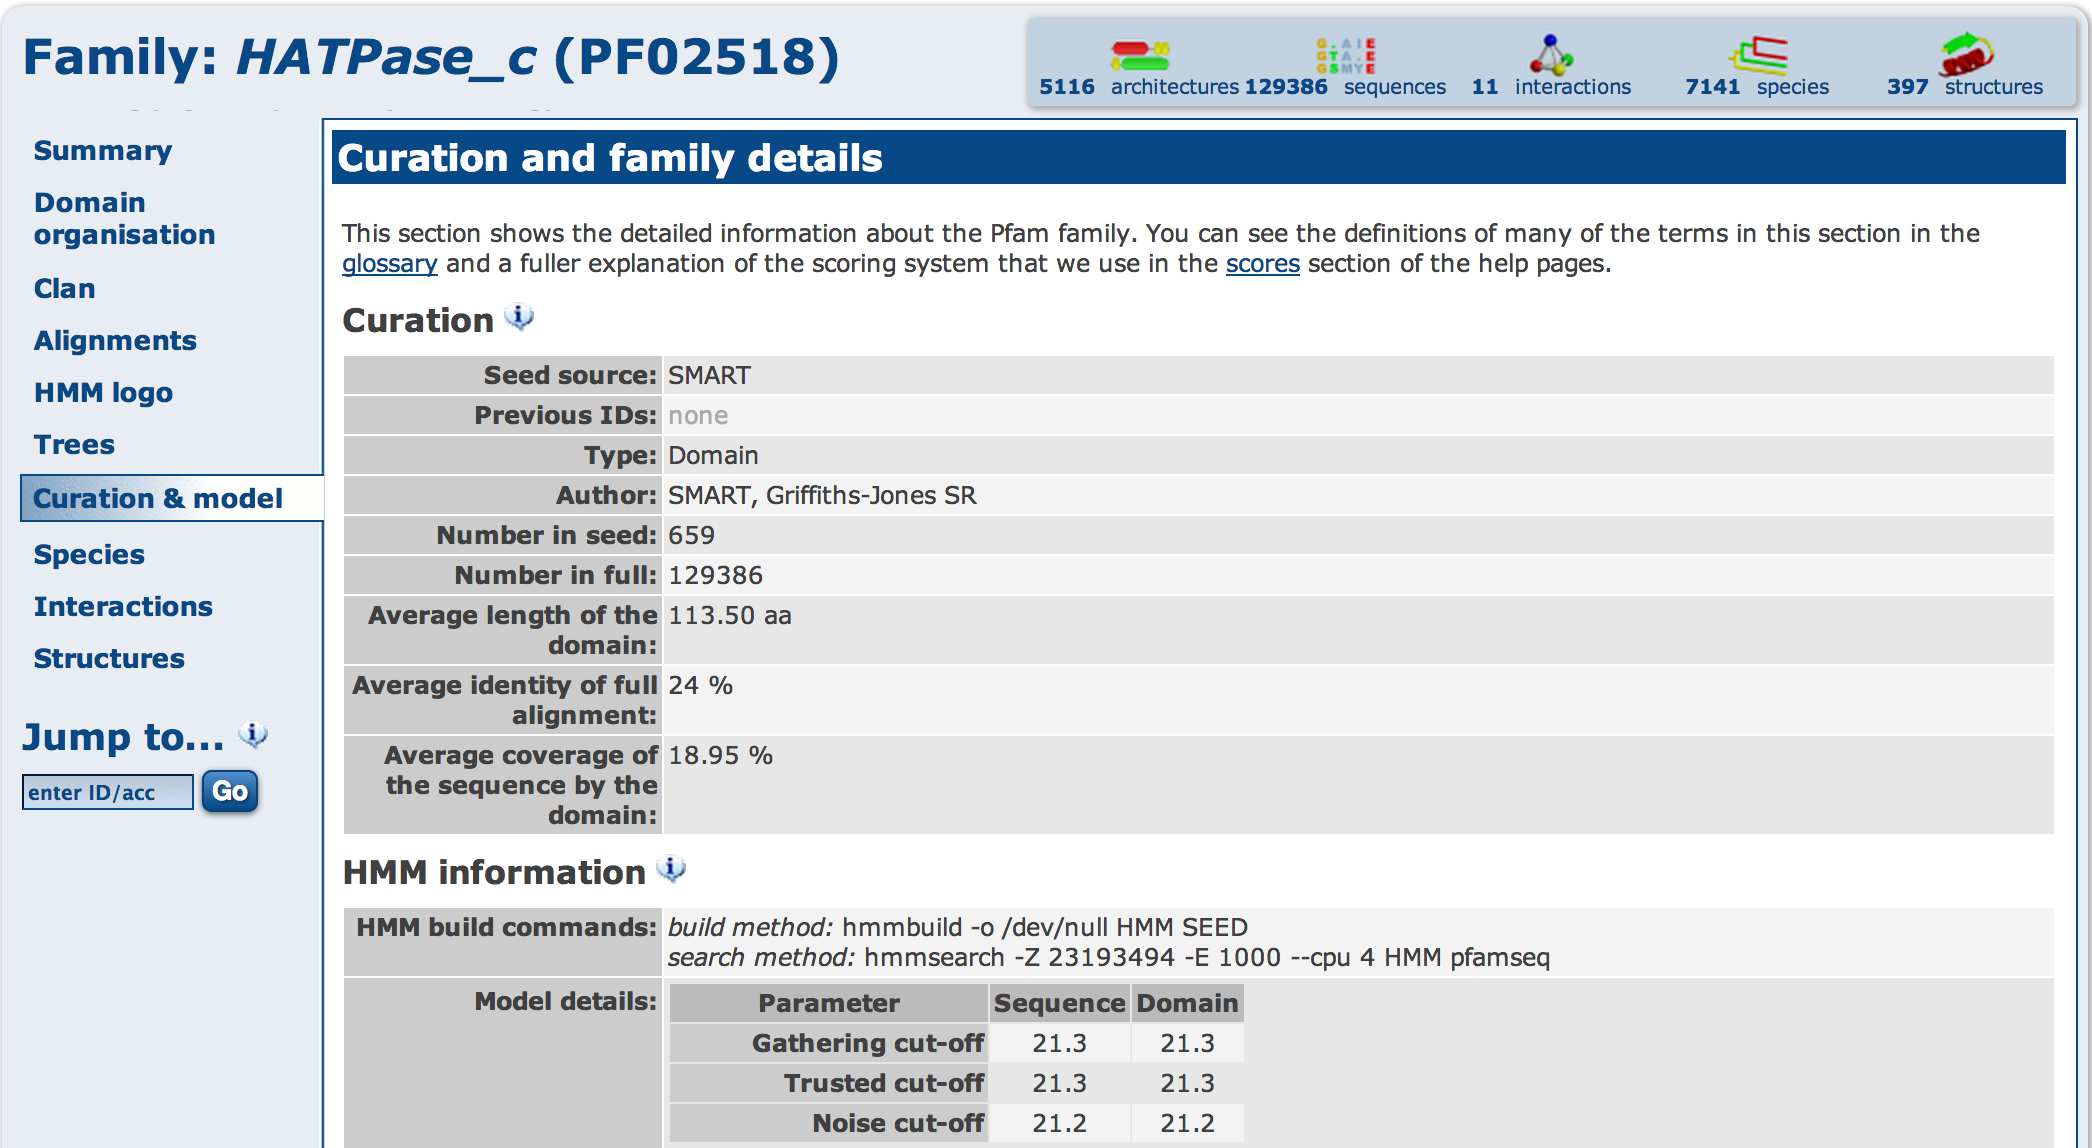
\includegraphics[width=0.8\textwidth]{images/pfam10} 
      \end{center}      
    \end{frame}

    \begin{frame}
      \frametitle{How PFam Works}   
      \begin{itemize}
        \item At the command-line, PFam works by running HMMer against published PFam databases
        \item Command-line use gives more control over HMMer settings, but less pretty output
        \item At the command-line, care must be taken over using GA, TC, NC cutoffs
      \end{itemize}
    \end{frame}

    % InterPro and RAST
    \subsection{InterPro and RAST}
    \begin{frame}
      \frametitle{InterPro}   
      \begin{itemize}
        \item Webserver for single sequences
        \item Local installations for whole-genome annotations
      \end{itemize}
      \begin{center}
        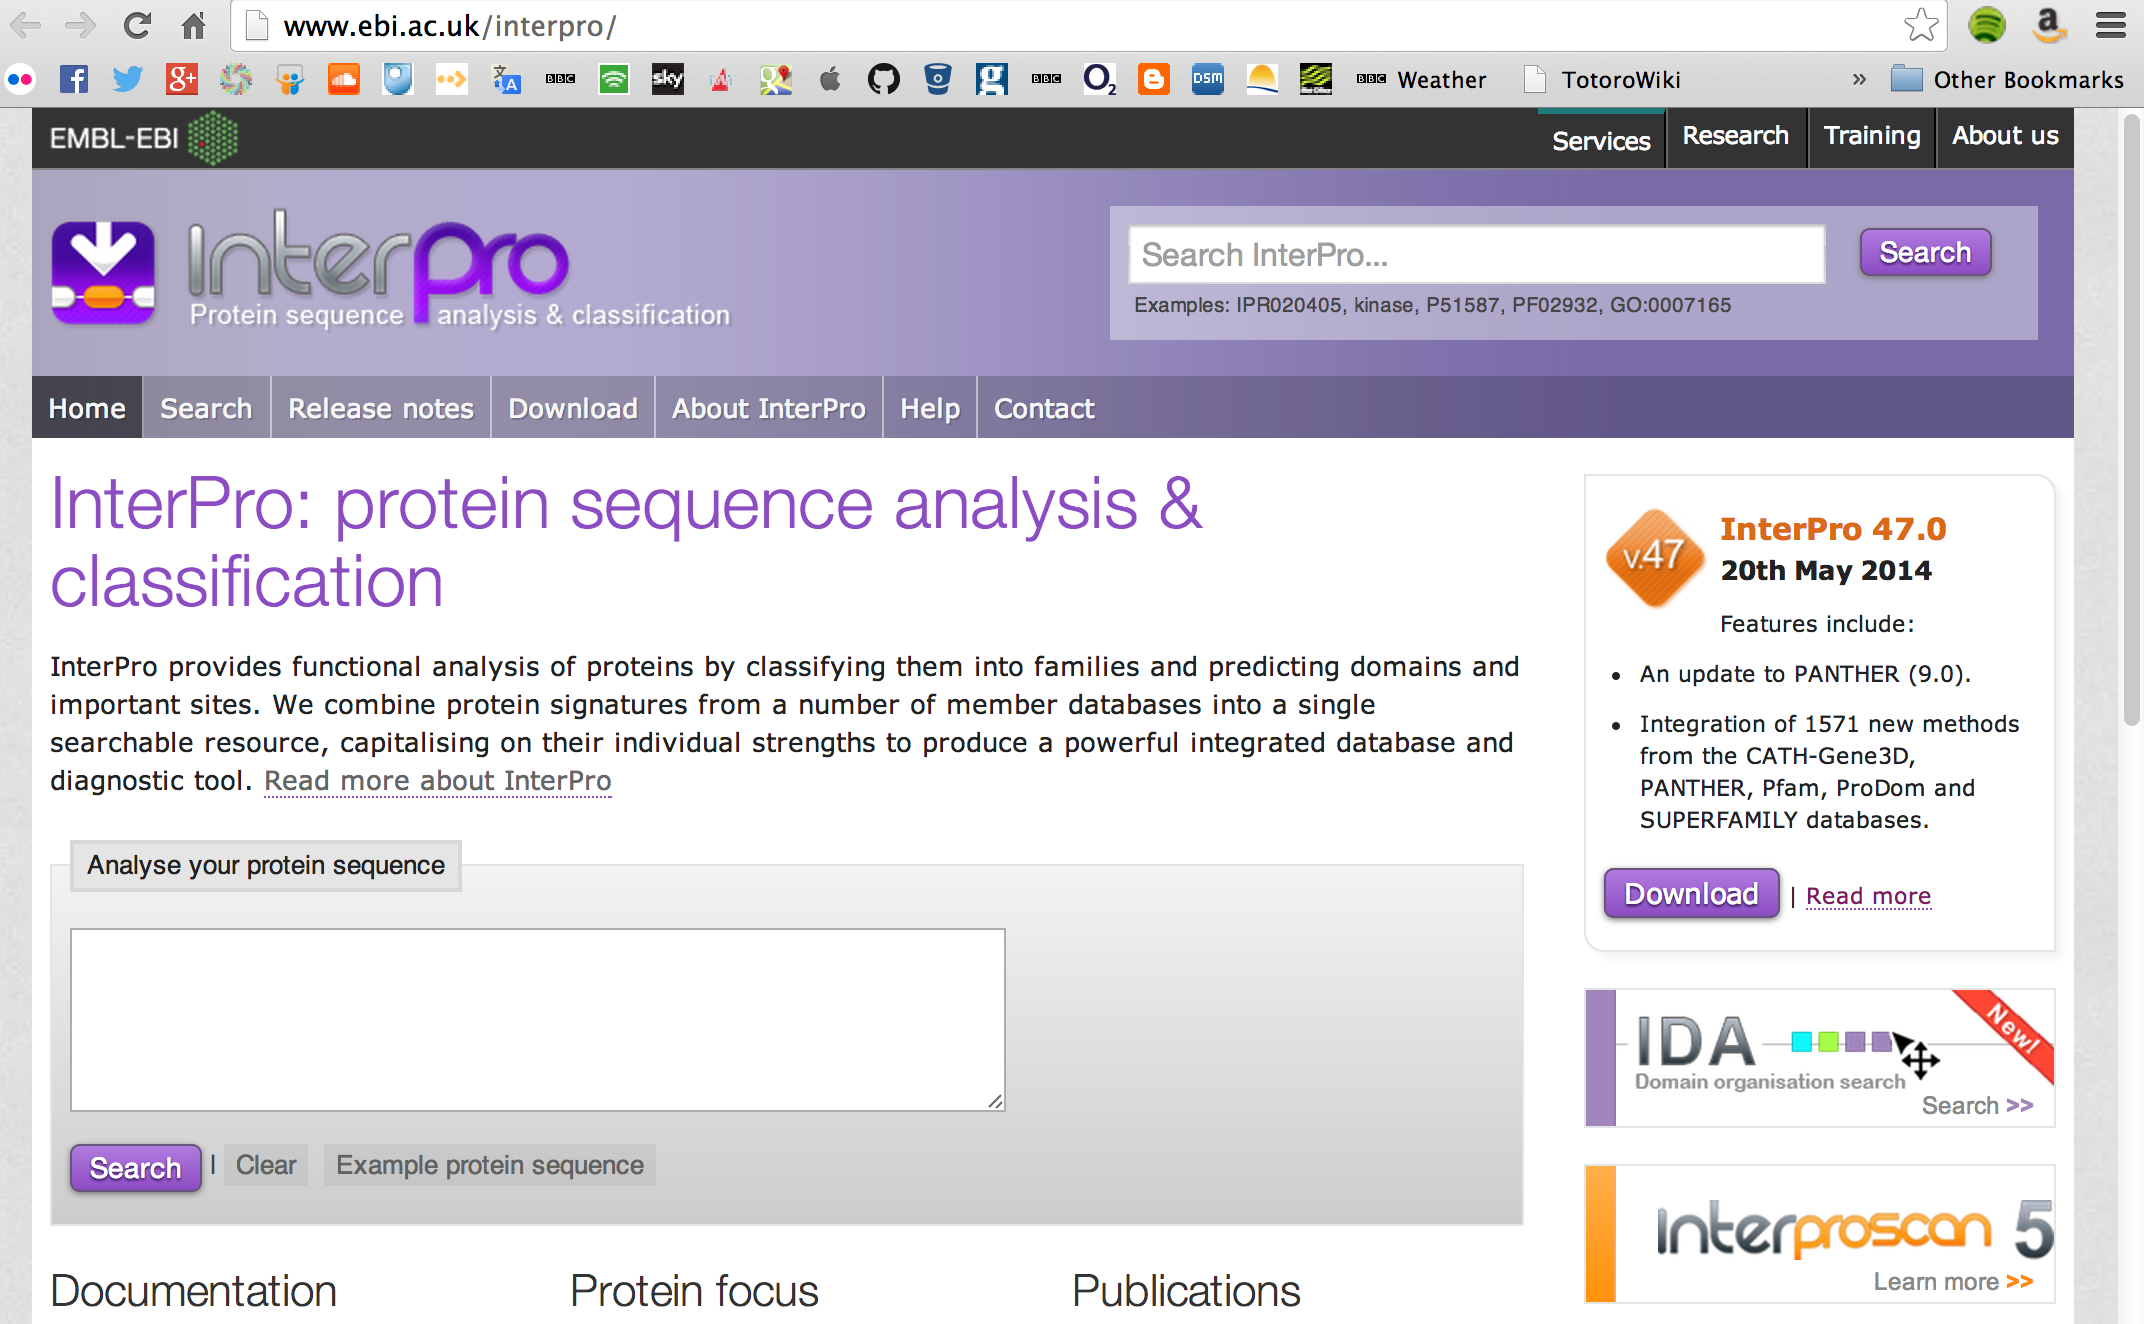
\includegraphics[width=0.8\textwidth]{images/interpro} 
      \end{center}        
    \end{frame}
    
    \begin{frame}
      \frametitle{How InterPro Works}   
      \begin{itemize}
        \item InterPro \url{http://www.ebi.ac.uk/interpro/} classifies proteins into families and predicts domains using a large number of tools, including:
        \begin{itemize}
          \item PFam, PROSITE, PRINTS, PANTHER, CATH
        \end{itemize}
        \item Predictive models of these databases are called `signatures'
      \end{itemize}
    \end{frame}

    \begin{frame}
      \frametitle{RAST}   
      \begin{itemize}
        \item Webserver for prokaryotic whole-genome annotation
        \item RAST calls genes as well as annotates them, but will accept your gene calls
      \end{itemize}
      \begin{center}
        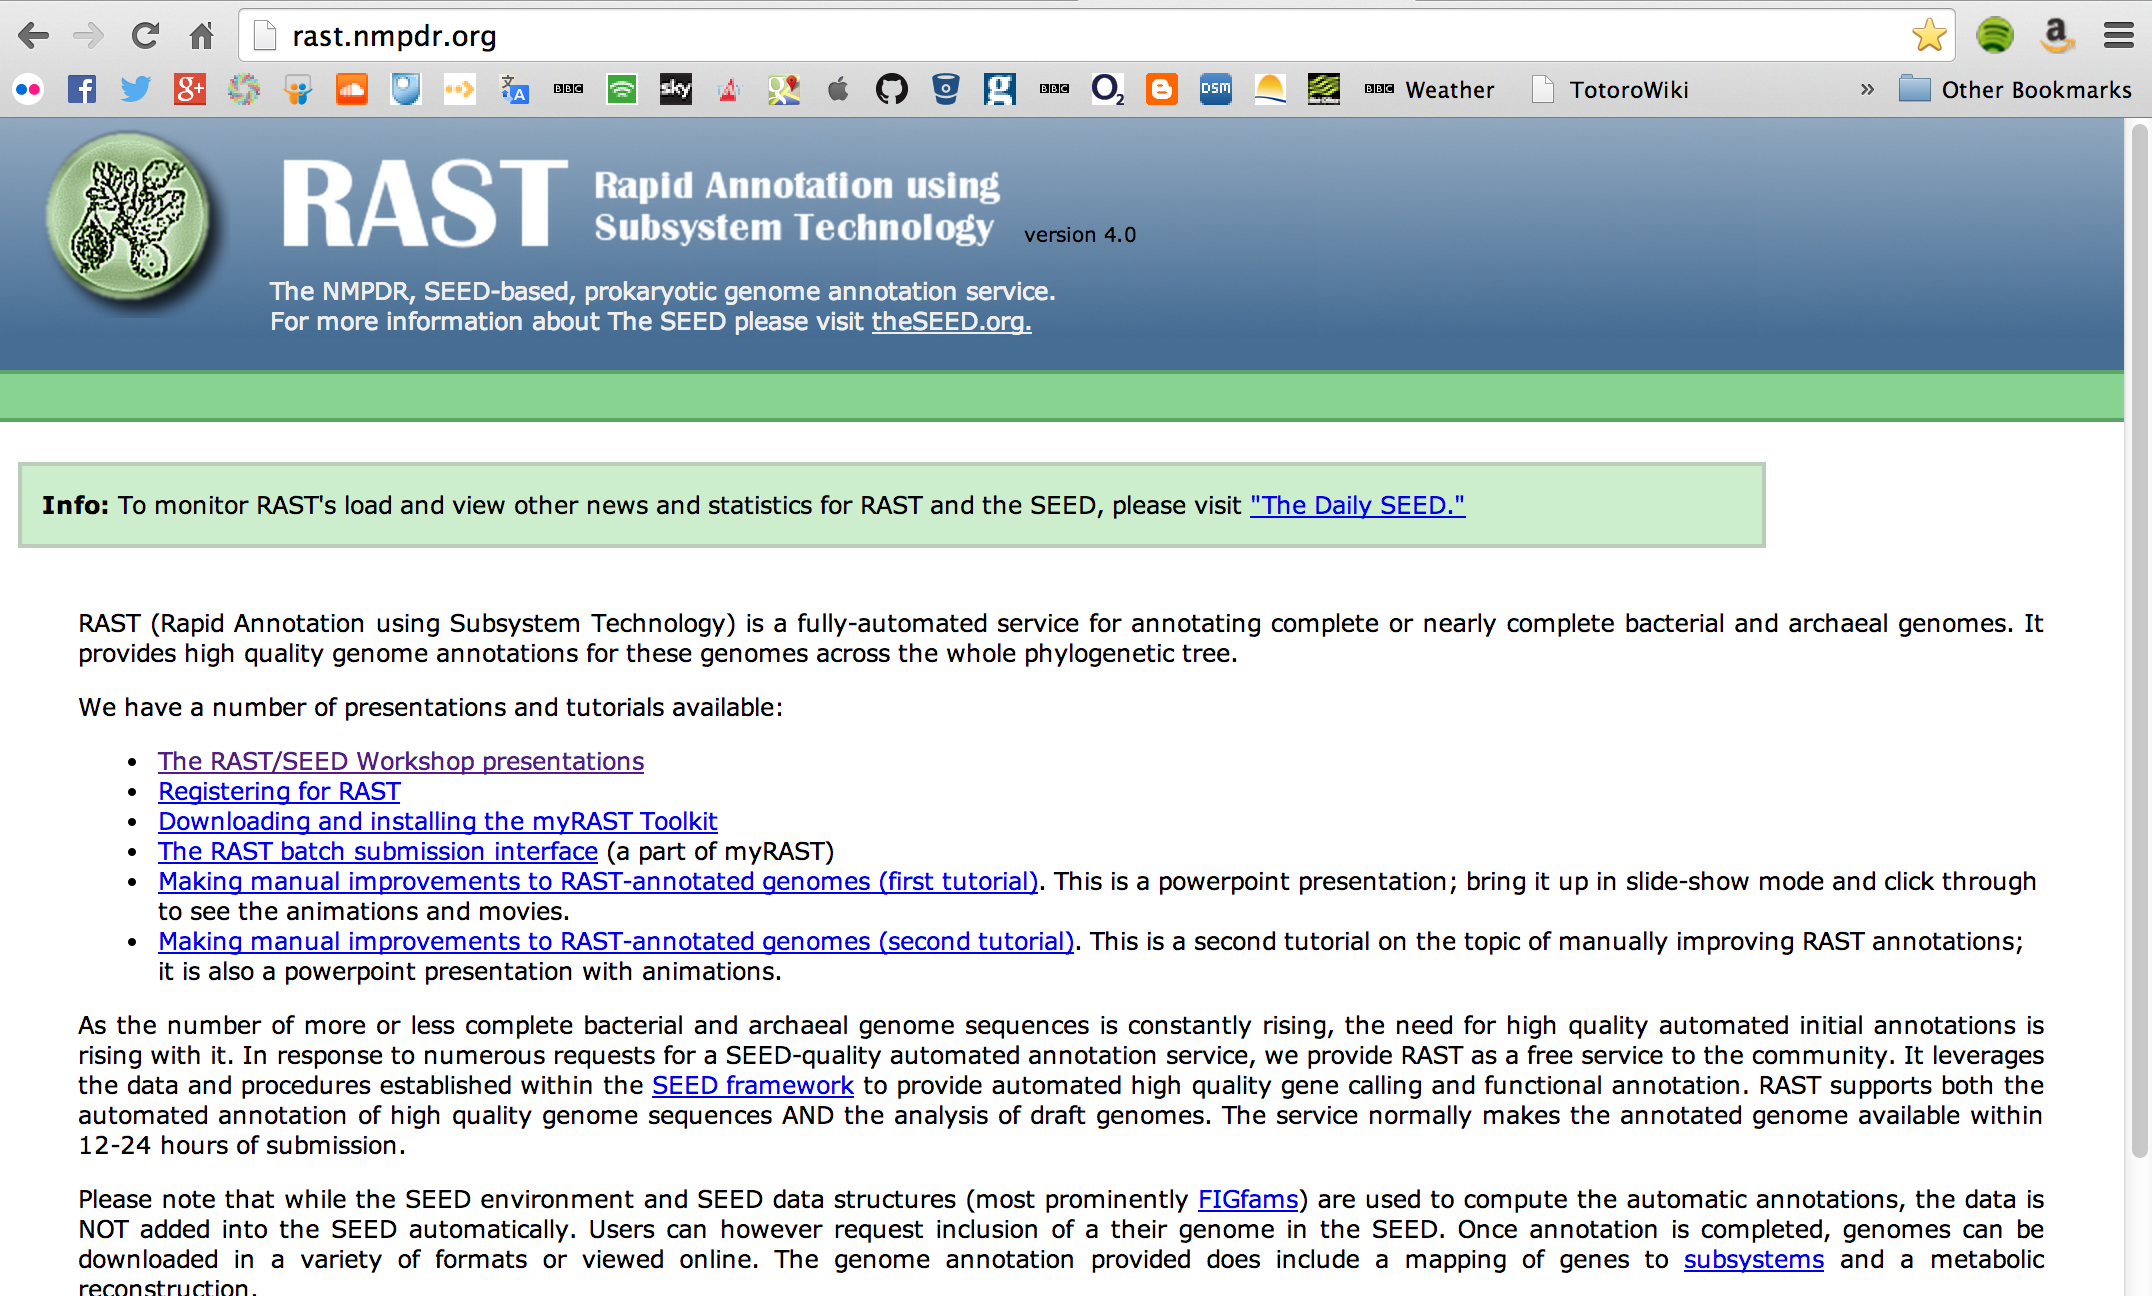
\includegraphics[width=0.8\textwidth]{images/rast} 
      \end{center}        
    \end{frame}

    \begin{frame}
      \frametitle{How RAST Works}   
      \begin{itemize} 
        \item Functional annotation is based on two SEED databases
        \begin{itemize}
          \item [A-SEED] Annotator SEED - representative high-quality
          \item [P-SEED] PATRIC-SEED - all prokaryotic genomes
        \end{itemize}
        \item SEEDs divided into FIGFams: families that are believed to implement the same function (isofunctional homologs)
        \item $k$-mer profile signatures are used to assign query sequences to FIGFams
      \end{itemize}
    \end{frame}

    \begin{frame}
      \frametitle{Your InterPro and RAST annotation data}
      We've already prepared these files for you:
      \begin{itemize}
        \item InterPro raw output: \texttt{chr*\_iprscan.raw}
        \item RAST output: \texttt{chr*\_RAST.gff}
      \end{itemize}
    \end{frame}

% [fragile] frames must end with \end{frame} directly following a newline, or they break!
  \begin{frame}[fragile]
    \frametitle{Visualisation of InterPro/RAST data in Artemis}
    InterPro raw output is not in a standard format
\begin{lstlisting}[language=bash]
$ head chrA_iprscan.raw 
chrA_04004	7A8F7B9C0479F48C	368	HMMPfam	PF06674	DUF1176	29	360	6.499999999999917E-49	T	23-Mar-2012	IPR009560	Protein of unknown function DUF1176	
chrA_04005	128211B8B939DE6B	365	HMMPfam	PF06674	DUF1176	32	358	1.2000000000000004E-61	T	23-Mar-2012	IPR009560	Protein of unknown function DUF1176	
chrA_04009	9E5C628D590CC7AE	1342	HMMPfam	PF04565	RNA_pol_Rpb2_3	513	582	1.4999999999999956E-29	T	23-Mar-2012	IPR007645	RNA polymerase Rpb2, domain 3	Molecular Function: DNA binding (GO:0003677), Molecular Function: DNA-directed RNA polymerase activity (GO:0003899), Biological Process: transcription, DNA-dependent (GO:0006351)
\end{lstlisting}
    Need to use \texttt{converter.pl} - skipping this for time
\end{frame}

% [fragile] frames must end with \end{frame} directly following a newline, or they break!
  \begin{frame}[fragile]
    \frametitle{Visualisation of InterPro/RAST data in Artemis}
    RAST will give us GFF, suitable for Artemis
\begin{lstlisting}[language=bash]
$ head chrA_RAST.gff
##gff-version 3
chrA	Prodigal_v2.00	CDS	3	1430	187.7	+	0	ID=chrA_00001;Alias=fig|556.22.peg.1;Name=Chromosomal replication initiator protein DnaA
chrA	Prodigal_v2.00	CDS	1435	2535	185.6	+	0	ID=chrA_00002;Alias=fig|556.22.peg.2;Name=DNA polymerase III beta subunit (EC 2.7.7.7);Ontology_term=KEGG_ENZYME:2.7.7.7
chrA	Prodigal_v2.00	CDS	2676	3761	146.2	+	0	ID=chrA_00003;Alias=fig|556.22.peg.3;Name=DNA recombination and repair protein RecF
\end{lstlisting}
\end{frame}

    \begin{frame}
      \frametitle{RAST}   
      GFF can be imported in the usual way
      \begin{center}
        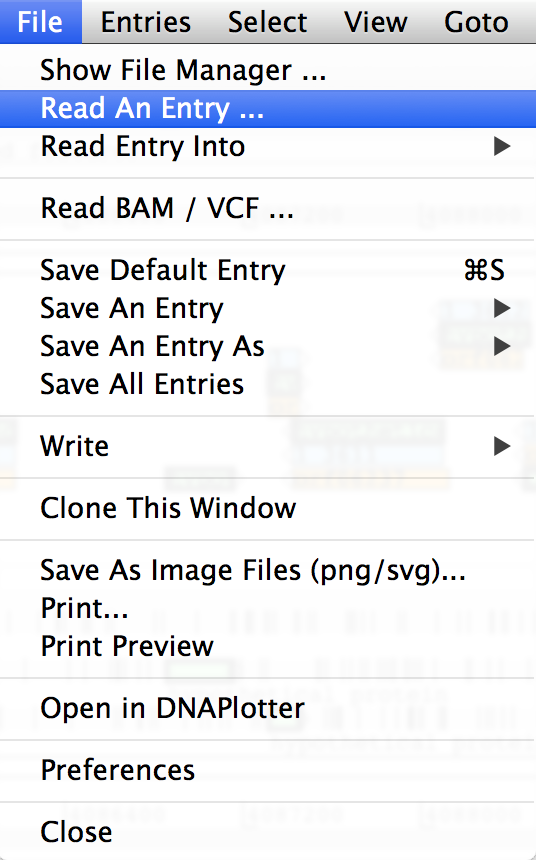
\includegraphics[width=0.3\textwidth]{images/rast0} 
      \end{center}        
    \end{frame}

    \begin{frame}
      \frametitle{RAST}   
      CDS predictions can be stacked
      \begin{center}
        \includegraphics[width=0.4\textwidth]{images/rast1} 
      \end{center}        
    \end{frame}

    \begin{frame}
      \frametitle{RAST}   
      Predictions are in good agreement, and annotation visible
      \begin{center}
        \includegraphics[width=0.9\textwidth]{images/rast2} 
      \end{center}        
    \end{frame}

    \begin{frame}
      \frametitle{Automated Functional Prediction}   
      \framesubtitle{Lessons learned}   
      \begin{itemize}
        \item Many alternative algorithms and databases are available 
        \item Integrated solutions (e.g. InterPro) are available
        \item Faster and larger-scale options tend to be more approximate
        \item How good is the agreement between alternatives?
        \item Automated annotations are a starting point, not a destination
      \end{itemize}
    \end{frame}

  % Gene Comparisons
  \section{Gene Comparisons}
    \begin{frame}
      \frametitle{Methods}   
      Most involve annotation transfer by sequence homology. \\
      Much is dependent on the quality of the alignment, and training set annotation.
      \begin{itemize}
        \item (Blast2GO \url{http://www.blast2go.com/b2ghome})
        \item (KEGG Automatic Annotation Server \url{http://www.genome.jp/kegg/kaas/})
        \item PFam \url{http://www.sanger.ac.uk/resources/databases/pfam.html}
        \item InterProScan \url{http://www.ebi.ac.uk/interpro/interproscan.html}
        \item RAST \url{http://rast.nmpdr.org/}
      \end{itemize}
    \end{frame}

    % BLAST/RBBH against known sequences to transfer function
    \subsection{BLAST}
% [fragile] frames must end with \end{frame} directly following a newline, or they break!
  \begin{frame}[fragile]
    \frametitle{Download Reference Sequences}
    Change directory to \texttt{chromosomes}, download reference protein data, and return to workspace
\begin{lstlisting}[language=bash]
$ wget ftp://ftp.ncbi.nih.gov/genomes/Bacteria/Pectobacterium_atrosepticum_SCRI1043_uid57957/NC_004547.faa
\end{lstlisting}
\end{frame}

    \begin{frame}
      \frametitle{Save CDS Annotation from Artemis}   
      Select all \texttt{prodigal} predicted CDS
      \begin{center}
        \includegraphics[width=0.6\textwidth]{images/export1}     
      \end{center}        
    \end{frame}

    \begin{frame}
      \frametitle{Save CDS Annotation from Artemis}   
      Choose to write protein sequences
      \begin{center}
        \includegraphics[width=0.6\textwidth]{images/export2}     
      \end{center}        
    \end{frame}

    \begin{frame}
      \frametitle{Save CDS Annotation from Artemis}   
      Select an output filename, e.g. \texttt{chrA\_prodigal.fasta}
      \begin{center}
        \includegraphics[width=0.6\textwidth]{images/export3}     
      \end{center}        
    \end{frame}


\begin{frame}
\frametitle{Reciprocal Best BLAST Hits (RBBH)}
\begin{itemize}
\item To compare our proteins to \texttt{NC\_004547.faa} reference set...
\item BLAST reference proteins against our proteins
\item BLAST our proteins against reference proteins
\item Pairs with each other as Best BLAST Hit are called an RBBH
\end{itemize}
\end{frame}

    \begin{frame}
      \frametitle{One-way BLAST vs RBBH}   
      One-way BLAST includes many low-quality hits
        \includegraphics[width=0.3\textwidth]{images/rbbh1}
        \includegraphics[width=0.33\textwidth]{images/rbbh2}
        \includegraphics[width=0.34\textwidth]{images/rbbh3}
    \end{frame}

    \begin{frame}
      \frametitle{One-way BLAST vs RBBH}   
      Reciprocal best BLAST hits remove many low-quality matches
        \includegraphics[width=0.3\textwidth]{images/rbbh4}
        \includegraphics[width=0.34\textwidth]{images/rbbh5}
        \includegraphics[width=0.34\textwidth]{images/rbbh6}
    \end{frame}

\begin{frame}
\frametitle{Reciprocal Best BLAST Hits (RBBH)}
\begin{itemize}
\item Pairs with each other as best BLAST hit are called an RBBH
\item Should filter on percentage identity and alignment length
\item RBBH pairs are candidate orthologues
\begin{itemize}
  \item (most orthologues will be RBBH, but the relationship is complicated)
\end{itemize}
\end{itemize}
(We have a tool for this on our in-house Galaxy server)
\end{frame}

% Test data generated locally using FASTA protein files made with Artemis,
% and the underlying Python script for my Galaxy BLAST RBH tool available
% from https://github.com/peterjc/galaxy_blast/tree/master/tools/blast_rbh
% Here I *DID NOT* import minimum coverage or identity thresholds!
%
% /mnt/galaxy/galaxy_blast/tools/blast_rbh/blast_rbh.py NC_004547.faa chrA_prodigal.fasta -o rbbh_ref_vs_chrA_prodigal.tab -t blastp -a prot
% /mnt/galaxy/galaxy_blast/tools/blast_rbh/blast_rbh.py NC_004547.faa chrB_prodigal.fasta -o rbbh_ref_vs_chrB_prodigal.tab -t blastp -a prot
% /mnt/galaxy/galaxy_blast/tools/blast_rbh/blast_rbh.py NC_004547.faa chrC_prodigal.fasta -o rbbh_ref_vs_chrC_prodigal.tab -t blastp -a prot
% /mnt/galaxy/galaxy_blast/tools/blast_rbh/blast_rbh.py NC_004547.faa chrD_prodigal.fasta -o rbbh_ref_vs_chrD_prodigal.tab -t blastp -a prot

% Multiple Sequence Alignment
\subsection{Multiple Sequence Alignment}

\begin{frame}
\frametitle{Quick Outline of MSA}
\begin{itemize}
  \item More difficult than pairwise alignment - no quick algorithm for optimal alignment
  \item Many methods progressive:
  \begin{enumerate}
    \item Build rough tree
    \item Conduct pairwise alignments from leaves to root
  \end{enumerate}
  \item Tree-based progressive methods highly dependent on initial tree$\ldots$
  \item Alignments can be compared directly (M-COFFEE)
\end{itemize}
\end{frame}

\begin{frame}
\frametitle{Example protein set MSA}
The example file \texttt{glucanase.fasta} contains:
\begin{itemize}
\item Reference protein \texttt{YP\_052458.1}, an endo-1,4-D-glucanase
\item Its RBBH from the prodigal gene predictions on \texttt{chrA.fasta}
\item Its RBBH from the prodigal gene predictions on \texttt{chrB.fasta}
\item Its RBBH from the prodigal gene predictions on \texttt{chrC.fasta}
\item Its RBBH from the prodigal gene predictions on \texttt{chrD.fasta}
\end{itemize}
If these are all orthologues, they should align nicely.
\end{frame}

\begin{frame}[fragile]
\frametitle{Clustal Omega MSA example}
Using example FASTA file of sequences:
\begin{lstlisting}[language=bash]
$ clustalo -i glucanase.fasta -o glucanase_clustalo.aln --outfmt=clustal
\end{lstlisting}
\end{frame}

\begin{frame}[fragile]
\frametitle{T-COFFEE MSA example}
Using same FASTA file of sequences:
%note that M-COFFEE performs consensus MSA using several methods
%but will they all be installed?
\begin{lstlisting}[language=bash]
$ t_coffee -infile glucanase.fasta -outfile glucanase_tcoffee.aln
\end{lstlisting}
\end{frame}

\begin{frame}[fragile]
\frametitle{JalView example}
Visualisation of the two MSAs generated above with JalView:
\begin{lstlisting}[language=bash]
$ Jalview &
\end{lstlisting}
\begin{itemize}
\item Menu ``File'', ``Input Alignment'', ``from File''.
\item Select ``Clustal (.aln)'' for the file type
\item Select your generated alignment file.
\end{itemize}
\end{frame}

\begin{frame}[fragile]
\frametitle{Clustal Omega \& T-COFFEE alignments in JalView}
\begin{center}
%TODO - Crop
Clustal Omega: \\
\includegraphics[width=\textwidth]{images/glucanase_clustalo.png} \\
T-COFFEE: \\
\includegraphics[width=\textwidth]{images/glucanase_tcoffee.png}
\end{center}
\end{frame}

\begin{frame}[fragile]
\frametitle{Clustal Omega \& T-COFFEE alignments in JalView}
\begin{center}
\begin{itemize}
\item Clustal Omega \& T-COFFEE gave different alignments
    \begin{itemize}
    \item e.g. region in red, and many more cropped on right
    \end{itemize}
\item The residues are coloured using the BLOSUM62 score
\item The proteins from draft chromosomes A, B, C and D are...
    \begin{itemize}
    \item Very similar to each other
    \item Only $30$ -- $35\%$ identical to the reference protein
    \item Probably \textit{not} orthologues of the reference protein
    \item Include minimum identity and coverage thresholds for RBBH!
    \end{itemize}
\end{itemize}
\end{center}
\end{frame}

\begin{frame}[fragile]
\frametitle{In Conclusion}
\begin{center}
\begin{itemize}
\item The tools you use will be task-dependent, but some things are universal$\ldots$
\begin{itemize}
  \item Good experimental design (including BLAST searches, etc.)
  \item Keeping accurate records for reproduction/replication
  \item Validation/sanity checking of results
  \item Comparison and benchmarking of methods
  \item (Cross-)validation of predictive methods
  \item Everything gets easier with practice
\end{itemize}
\end{itemize}
\end{center}
\end{frame}


%% HMMer
%\subsection{HMMer}
%
%    \begin{frame}
%      \frametitle{Quick Outline of HMMer}   
%      HMMs are profile methods, differ from sequence alignment algorithms like BLAST \\
%      NOTE: HMMer alignments explicitly account for alignment uncertainty, BLAST alignments do not.
%    \end{frame}
%
%    \begin{frame}
%      \frametitle{HMMer vs BLAST comparison}   
%      Example from chromosome vs reference \\
%      One BLASTP search \\
%      One PHMMER search
%    \end{frame}

% Gene/ORF finding
%\section{Gene Prediction}
%\subsection{Finding Open Reading Frames (ORFs) within Artemis}
%
%\begin{frame}
%    \frametitle{Finding Open Reading Frames (ORFs) within Artemis}
%    \begin{itemize}
%      \item<1-> Set genetic code
%      \begin{itemize}
%        \item Main window menu, ``Options'',
%        \item ``11. Bacterial and plant plastid''
%      \end{itemize}
%      \item<2-> Top menu, ``Create'', ``Mark empty ORFs ...''
%      \item<2-> Set minimum open reading frame size, e.g. 100 aa
%      \item<2-> CDS features created, defaulting to pale blue.
%    \end{itemize}
%\end{frame}
%
%\begin{frame}
%    \frametitle{Adjusting start of CDS features en mass}
%    \begin{itemize}
%      \item<1-> Top menu, ``Select all CDS Features'',
%      \item<1-> Top menu, ``Trim Selected Features'', ``To Any'' \\
%           (or ``To Met'' if you prefer the canonical start codon)
%      \item<2-> Un-trimmable features now selected...
%      \item<2-> Press delete to remove them (!) \\
%           (can we assume these are all not real genes?)
%    \end{itemize}
%\end{frame}
%
%\begin{frame}
%    \frametitle{Artemis Feature Selector}
%    \begin{itemize}
%	  \item<1-> After editing, check for any short CDS entries
%	  \item<1-> Top menu, ``Select'', ``Feature Selector...''
%	  \item<1-> Use up to length 300bp, click ``View''
%	  \item<1-> Use up to length 300bp, click ``Select'', delete them?
%    \end{itemize}
%\end{frame}

%\subsection{Basic Gene Finding}
%
%\section{Functional Prediction}
%
%\section{Gene Comparison}

% etc
\end{document}
